\RequirePackage[l2tabu, orthodox]{nag}

%\documentclass[]{article}
\documentclass[11pt]{scrartcl}
\usepackage[usename, dvipsnames]{xcolor}
\usepackage[pdfencoding=auto]{hyperref}
\usepackage[msc-links]{amsrefs}
\usepackage{cleveref} % use \cref{}, automatically deduces theorem, proposition, etc
\usepackage[mathletters]{ucs}
\usepackage[utf8]{inputenc}
\usepackage[T1]{fontenc}
\usepackage{datetime}

\usepackage{array}
\usepackage{mathtools}
\usepackage{amsmath, amsthm, amssymb, amsfonts, amsxtra, amscd, thmtools}
\let\proof\relax
\let\endproof\relax

% Boxes around theorem environments.
\usepackage[many]{tcolorbox}

\usepackage{color}
%\usepackage{unicode-math}
\usepackage{newunicodechar}
\newunicodechar{ε}{\varepsilon}
\newunicodechar{δ}{\delta}
\newunicodechar{µ}{\mu}
\newunicodechar{→}{\to}
\newunicodechar{≤}{\leq}
\newunicodechar{∈}{\in}
\newunicodechar{⊆}{\subseteq}
\newunicodechar{Λ}{\Lambda}
\newunicodechar{∞}{\infty}
\newunicodechar{×}{\times}
\everymath{\displaystyle}



\usepackage{microtype}
\usepackage[pdfencoding=auto]{hyperref}
\usepackage{bookmark}
\usepackage{booktabs}
\usepackage{todonotes}
\usepackage[msc-links]{amsrefs}
\usepackage{cleveref} % use \cref{}, automatically deduces theorem, proposition, etc
\usepackage{csquotes}
\usepackage{longtable}
\usepackage{tabularx}
\usepackage{bbm}
% Creating multiple types of index
\usepackage{imakeidx}

% Remove indentation for new paragraphs
\usepackage{parskip}
% But leave space before amsthm environments
\makeatletter
\def\thm@space@setup{%
  \thm@preskip=2em
  \thm@postskip=2em
}
\makeatother


\usepackage{stmaryrd}
\usepackage{adjustbox}
\usepackage{centernot}
% \centernot\whatever


% Better indicator function
\usepackage{bbm}
\newcommand{\indic}[1]{\mathbbm{1} \left[ {#1} \right] }

% Highlight quote
\usepackage{environ}
\definecolor{camel}{rgb}{0.76, 0.6, 0.42}
\definecolor{babyblue}{rgb}{0.54, 0.81, 0.94}
\definecolor{block-gray}{gray}{0.85}
\NewEnviron{myblock}
{\colorbox{block-gray}{%
\parbox{\dimexpr\linewidth-2\fboxsep\relax}{%
\small\addtolength{\leftskip}{10mm}
\addtolength{\rightskip}{10mm}
\BODY}}
}
\renewcommand{\quote}{\myblock}
\renewcommand{\endquote}{\endmyblock}

% Nice math font that journals use
%\usepackage[lite]{mtpro2}
%\usepackage{mathrsfs}
%\usepackage{mathptmx}
\usepackage{lmodern}
%\usepackage[sc]{mathpazo}

% Theorem Styles
\usepackage[framemethod=tikz]{mdframed}

\theoremstyle{definition}
\newtheorem{exercise}{Exercise}[section]
\newtheorem{solution}{Solution}

% Theorem Style
\newtheoremstyle{theorem}% name
  {0em}%         Space above, empty = `usual value'
  {1em}%         Space below
  {\normalfont}% Body font
  {\parindent}%         Indent amount (empty = no indent, \parindent = para indent)
  {\bfseries}% Thm head font
  {.}%        Punctuation after thm head
  {\newline}% Space after thm head: \newline = linebreak
  {\thmname{#1}\thmnumber{ #2}\thmnote{\itshape{(#3)}}}%
\theoremstyle{theorem}
\tcolorboxenvironment{theorem}{
  boxrule=0pt,
  boxsep=0pt,
  breakable,
  enhanced jigsaw,
  fonttitle={\large\bfseries},
  opacityback=0.8,
  colframe=cyan,
  borderline west={4pt}{0pt}{orange},
  attach title to upper={}
}
\newtheorem{theorem}{Theorem}[section]

% Proposition Style
\tcolorboxenvironment{proposition}{
  boxrule=1pt,
  boxsep=0pt,
  breakable,
  enhanced jigsaw,
  opacityback=0.0,
  colframe=cyan
}
\newtheorem{proposition}[theorem]{Proposition}
\tcolorboxenvironment{lemma}{
  boxrule=1pt,
  boxsep=0pt,
  breakable,
  enhanced jigsaw,
  opacityback=0.2,
  colframe=cyan
}
\newtheorem{lemma}[theorem]{Lemma}
% Claim
\tcolorboxenvironment{claim}{
  boxrule=1pt,
  boxsep=0pt,
  breakable,
  enhanced jigsaw,
  opacityback=0.2,
  colframe=cyan
}
\newtheorem{claim}[theorem]{Claim}


% Corollary
\tcolorboxenvironment{corollary}{
  colback=cyan,
  boxrule=1pt,
  boxsep=0pt,
  breakable,
  enhanced jigsaw,
  opacityback=0.1,
  colframe=cyan
}
\newtheorem{corollary}[theorem]{Corollary}

% Proof Style
\newtheoremstyle{proof}% name
  {0em}%         Space above, empty = `usual value'
  {2em}%         Space below
  {\normalfont}% Body font
  {\parindent}%         Indent amount (empty = no indent, \parindent = para indent)
  {\itshape}% Thm head font
  {.}%        Punctuation after thm head
  {\newline}% Space after thm head: \newline = linebreak
  {\thmname{#1} \thmnote{\itshape{(#3)}}}%         Thm head spec
\theoremstyle{proof}
\tcolorboxenvironment{proof}{
  colback=camel,
  opacityfill=0.25,
  boxrule=1pt,
  boxsep=0pt,
  breakable,
  enhanced jigsaw
}
\newtheorem*{pf}{Proof}
\newenvironment{proof}
{\pushQED{$\qed$}\pf}
{\par\popQED\endpf}

% Definition Style
\newtheoremstyle{definition}% name
  {0em}%         Space above, empty = `usual value'
  {2em}%         Space below
  {\normalfont}% Body font
  {\parindent}%         Indent amount (empty = no indent, \parindent = para indent)
  {\bfseries}% Thm head font
  {.}%        Punctuation after thm head
  {\newline}% Space after thm head: \newline = linebreak
  {}%         Thm head spec
\theoremstyle{definition}
\tcolorboxenvironment{definition}{
  colback=babyblue,
  boxrule=0pt,
  boxsep=0pt,
  opacityfill=0.45,
  breakable,
  enhanced jigsaw,
  borderline west={4pt}{0pt}{blue},
  colbacktitle={babyblue},
  coltitle={black},
  fonttitle={\large\bfseries},
  attach title to upper={},
}
\newtheorem{definition}{Definition}[theorem]

% Break Environment
\makeatletter
\newtheoremstyle{break}% name
  {}%         Space above, empty = `usual value'
  {2em}%         Space below
  {
    \addtolength{\@totalleftmargin}{2.5em}
    \addtolength{\linewidth}{-2.5em}
    \parshape 1 2.5em \linewidth
  }% Body font
  {}%         Indent amount (empty = no indent, \parindent = para indent)
  {\bfseries}% Thm head font
  {.}%        Punctuation after thm head
  {\newline}% Space after thm head: \newline = linebreak
  {}%         Thm head spec
\makeatother

\theoremstyle{break}
\newtheorem{example}{Example}[section]

% Problem Style
\newtheoremstyle{problem} % name
  {0em}                   % Space above, empty = `usual value'
  {2em}                   % Space below
  {\normalfont}           % Body font
  {\parindent}            % Indent amount (empty = no indent, \parindent = para indent)
  {\itshape}              % Thm head font
  {}                      % Punctuation after thm head
  {\newline}              % Space after thm head: \newline = linebreak
  {\thmnote{\itshape{(#3)}}}     % Thm head spec
\theoremstyle{problem}
\tcolorboxenvironment{problem}{
  boxrule=1pt,
  boxsep=0pt,
  breakable,
  enhanced jigsaw,
  opacityback=0.0,
  colframe=cyan
}
\newtheorem{problem}{Problem}


%Pagination stuff.
\setlength{\topmargin}{-.3 in}
\setlength{\oddsidemargin}{0in}
\setlength{\evensidemargin}{0in}
\setlength{\textheight}{9.in}
\setlength{\textwidth}{6.5in}
% \pagestyle{empty} %removes page numbers.

% Inkscape figures from Vim
\usepackage{import}
\usepackage{pdfpages}
\usepackage{transparent}

\newcommand{\incfig}[1]{%
    \def\svgwidth{\columnwidth}
    \import{./figures/}{#1.pdf_tex}
}
%\pdfsuppresswarningpagegroup=1

% Pandoc-specific fixes
\providecommand{\tightlist}{%
  \setlength{\itemsep}{0pt}\setlength{\parskip}{0pt}}

% Tikz and Graphics
\usepackage{amscd}
\usepackage{tikz}
\usetikzlibrary{arrows, arrows.meta, cd, fadings, patterns, calc, decorations.markings, matrix, positioning}
\tikzfading[name=fade out, inner color=transparent!0, outer color=transparent!100]
\usepackage{pgfplots}
\pgfplotsset{compat=1.16}
\usepackage[inline]{asymptote}
\usepackage{tikz-layers}

%\usepackage{nath}
%\delimgrowth=1
\DeclarePairedDelimiter\qty{(}{)}

% Major Macros
\usepackage{graphicx}
\usepackage{float}
\DeclareFontFamily{U}{mathx}{\hyphenchar\font45}
\DeclareFontShape{U}{mathx}{m}{n}{
      <5> <6> <7> <8> <9> <10>
      <10.95> <12> <14.4> <17.28> <20.74> <24.88>
      mathx10
      }{}
\DeclareSymbolFont{mathx}{U}{mathx}{m}{n}
\DeclareMathSymbol{\bigtimes}{1}{mathx}{"91}

% Wide tikz equations
\newsavebox{\wideeqbox}
\newenvironment{wideeq}
  {\begin{displaymath}\begin{lrbox}{\wideeqbox}$\displaystyle}
  {$\end{lrbox}\makebox[0pt]{\usebox{\wideeqbox}}\end{displaymath}}



% Fancy chapter headers and footers
\usepackage{fancyhdr}

\pagestyle{fancy}
\fancyhf{}
\fancyhead[LE,RO]{\title}
\fancyhead[RE,LO]{\rightmark}
\fancyfoot[CE,CO]{\leftmark}
\fancyfoot[LE,RO]{\thepage}

\renewcommand{\headrulewidth}{2pt}
\renewcommand{\footrulewidth}{1pt}

% List of Theorems Attempt
\usepackage{etoolbox}
\makeatletter
\patchcmd\thmtlo@chaptervspacehack
  {\addtocontents{loe}{\protect\addvspace{10\p@}}}
  {\addtocontents{loe}{\protect\thmlopatch@endchapter\protect\thmlopatch@chapter{\thechapter}}}
  {}{}
\AtEndDocument{\addtocontents{loe}{\protect\thmlopatch@endchapter}}
\long\def\thmlopatch@chapter#1#2\thmlopatch@endchapter{%
  \setbox\z@=\vbox{#2}%
  \ifdim\ht\z@>\z@
    \hbox{\bfseries\chaptername\ #1}\nobreak
    #2
    \addvspace{10\p@}
  \fi
}
\def\thmlopatch@endchapter{}

\makeatother
\renewcommand{\thmtformatoptarg}[1]{ -- #1}
%\renewcommand{\listtheoremname}{List of definitions}

\newcommand{\ext}{\operatorname{Ext}}
\newcommand{\Ext}{\operatorname{Ext}}
\def\Endo{\operatorname{End}}
\def\Ind{\operatorname{Ind}}
\def\ind{\operatorname{Ind}}
\def\coind{\operatorname{Coind}}
\def\Res{\operatorname{Res}}
\def\Hol{\operatorname{Hol}}
\def\res{\operatorname{Res}}
\def\endo{\operatorname{End}}
\def\ind{\operatorname{Ind}}
\renewcommand{\AA}[0]{{\mathbb{A}}}
\DeclareMathOperator{\Exists}{\exists}
\DeclareMathOperator{\Forall}{\forall}
\newcommand{\Af}[0]{{\mathbb{A}}}
\newcommand{\CC}[0]{{\mathbb{C}}}
\newcommand{\CP}[0]{{\mathbb{CP}}}
\newcommand{\DD}[0]{{\mathbb{D}}}
\newcommand{\FF}[0]{{\mathbb{F}}}
\newcommand{\GF}[0]{{\mathbb{GF}}}
\newcommand{\GG}[0]{{\mathbb{G}}}
\newcommand{\HH}[0]{{\mathbb{H}}}
\newcommand{\HP}[0]{{\mathbb{HP}}}
\newcommand{\KK}[0]{{\mathbb{K}}}
\newcommand{\kk}[0]{{\Bbbk}}
\newcommand{\bbm}[0]{{\mathbb{M}}}
\newcommand{\NN}[0]{{\mathbb{N}}}
\newcommand{\OP}[0]{{\mathbb{OP}}}
\newcommand{\PP}[0]{{\mathbb{P}}}
\newcommand{\QQ}[0]{{\mathbb{Q}}}
\newcommand{\RP}[0]{{\mathbb{RP}}}
\newcommand{\RR}[0]{{\mathbb{R}}}
\newcommand{\SpSp}[0]{{\mathbb{S}}}
\renewcommand{\SS}[0]{{\mathbb{S}}}
\newcommand{\TT}[0]{{\mathbb{T}}}
\newcommand{\ZZ}[0]{{\mathbb{Z}}}
\newcommand{\ZnZ}[0]{\mathbb{Z}/n\mathbb{Z}}
\newcommand{\ZpZ}[0]{\mathbb{Z}/p\mathbb{Z}}
\newcommand{\Qp}[0]{\mathbb{Q}_{(p)}}
\newcommand{\Zp}[0]{\mathbb{Z}_{(p)}}
\newcommand{\Arg}[0]{\mathrm{Arg}}
\newcommand{\PGL}[0]{\mathrm{PGL}}
\newcommand{\GL}[0]{\mathrm{GL}}
\newcommand{\Gl}[0]{\mathrm{GL}}
\newcommand{\gl}[0]{\mathrm{GL}}
\newcommand{\mat}[0]{\mathrm{Mat}}
\newcommand{\Mat}[0]{\mathrm{Mat}}
\newcommand{\Rat}[0]{\mathrm{Rat}}
\newcommand{\Perv}[0]{\mathrm{Perv}}
\newcommand{\Gal}[0]{\mathrm{Gal}}
\newcommand{\Hilb}[0]{\mathrm{Hilb}}
\newcommand{\Quot}[0]{\mathrm{Quot}}
\newcommand{\Art}[0]{\mathrm{Art}}
\newcommand{\red}[0]{\mathrm{red}}
\newcommand{\alg}[0]{\mathrm{alg}}
\newcommand{\Pic}[0]{{\mathrm{Pic}~}}
\newcommand{\lcm}[0]{\mathrm{lcm}}
\newcommand{\maps}[0]{\mathrm{Maps}}
\newcommand{\maxspec}[0]{{\mathrm{maxSpec}~}}
\newcommand{\Tr}[0]{\mathrm{Tr}}
\newcommand{\adj}[0]{\mathrm{adj}}
\newcommand{\ad}[0]{\mathrm{ad}~}
\newcommand{\ann}[0]{\mathrm{Ann}}
\newcommand{\Ann}[0]{\mathrm{Ann}}
\newcommand{\arcsec}[0]{\mathrm{arcsec}}
\newcommand{\ch}[0]{\mathrm{char}~}
\newcommand{\Sp}[0]{{\mathrm{Sp}}}
\newcommand{\syl}[0]{{\mathrm{Syl}}}
\newcommand{\txand}[0]{{\text{ and }}}
\newcommand{\codim}[0]{\mathrm{codim}}
\newcommand{\txor}[0]{{\text{ or }}}
\newcommand{\txt}[1]{{\text{ {#1} }}}
\newcommand{\Gr}[0]{{\text{Gr}}}
\newcommand{\Aut}[0]{{\mathrm{Aut}}}
\newcommand{\aut}[0]{\mathrm{Aut}}
\newcommand{\Inn}[0]{{\mathrm{Inn}}}
\newcommand{\Out}[0]{{\mathrm{Out}}}
\newcommand{\mltext}[1]{\left\{\begin{array}{c}#1\end{array}\right\}}
\newcommand{\Fun}[0]{{\text{Fun}}}
\newcommand{\SL}[0]{{\text{SL}}}
\newcommand{\PSL}[0]{{\text{PSL}}}
\newcommand{\SO}[0]{{\text{SO}}}
\newcommand{\SU}[0]{{\text{SU}}}
\newcommand{\SP}[0]{{\text{SP}}}
\newcommand{\per}[0]{{\text{Per}}}
\newcommand{\loc}[0]{{\text{loc}}}
\newcommand{\Top}[0]{{\text{Top}}}
\newcommand{\Sch}[0]{{\text{Sch}}}
\newcommand{\sch}[0]{{\text{Sch}}}
\newcommand{\Set}[0]{{\text{Set}}}
\newcommand{\Sets}[0]{{\text{Set}}}
\newcommand{\Grp}[0]{{\text{Grp}}}
\newcommand{\Groups}[0]{{\text{Groups}}}
\newcommand{\Homeo}[0]{{\text{Homeo}}}
\newcommand{\Diffeo}[0]{{\text{Diffeo}}}
\newcommand{\MCG}[0]{{\text{MCG}}}
\newcommand{\set}[0]{{\text{Set}}}
\newcommand{\Tor}[0]{\text{Tor}}
\newcommand{\sets}[0]{{\text{Set}}}
\newcommand{\Sm}[0]{{\text{Sm}_k}}
\newcommand{\orr}[0]{{\text{ or }}}
\newcommand{\annd}[0]{{\text{ and }}}
\newcommand{\bung}[0]{\text{Bun}_G}
\newcommand{\const}[0]{{\text{const.}}}
\newcommand{\disc}[0]{{\text{disc}}}
\newcommand{\op}[0]{^\text{op}}
\newcommand{\id}[0]{\text{id}}
\newcommand{\im}[1]{\mathrm{im}({#1})}
\newcommand{\pt}[0]{{\{\text{pt}\}}}
\newcommand{\sep}[0]{^\text{sep}}
% \newcommand{\st}[0]{~{\text{s.t.}}~}
\newcommand{\tors}[0]{{\text{tors}}}
\newcommand{\tor}[0]{\text{Tor}}
\newcommand{\height}[0]{\text{ht}}
\newcommand{\cpt}[0]{\text{compact}}
\newcommand{\abs}[1]{{\left\lvert {#1} \right\rvert}}
\newcommand{\stack}[1]{\mathclap{\substack{ #1 }}} 
\newcommand{\qtext}[1]{{\quad \text{#1} \quad}}
\newcommand{\qst}[0]{{\quad \text{such that} \quad}}
\newcommand{\actsonl}[0]{\curvearrowleft}
\newcommand{\actson}[0]{\curvearrowright}
\newcommand{\bd}[0]{{\del}}
\newcommand{\bigast}[0]{{\mathop{\Large \ast}}}
\newcommand{\coker}[0]{\operatorname{coker}}
\newcommand{\cok}[0]{\operatorname{coker}}
\newcommand{\conjugate}[1]{{\overline{{#1}}}}
\newcommand{\converges}[1]{\overset{#1}}
\newcommand{\correspond}[1]{\theset{\substack{#1}}}
\newcommand{\cross}[0]{\times}
\newcommand{\by}[0]{\times}
\newcommand{\dash}[0]{{\hbox{-}}}
\newcommand{\dd}[2]{{\frac{\partial #1}{\partial #2}\,}}
\newcommand{\definedas}[0]{\coloneqq}
\newcommand{\da}[0]{\coloneqq}
\newcommand{\del}[0]{{\partial}}
\newcommand{\directlim}[0]{\varinjlim}
\newcommand{\disjoint}[0]{{\coprod}}
\newcommand{\divides}[0]{{~\Bigm|~}}
\newcommand{\dual}[0]{^\vee}
\newcommand{\sm}[0]{\setminus}
\newcommand{\smz}[0]{\setminus\theset{0}}
\newcommand{\eps}[0]{\varepsilon}
\newcommand{\equalsbecause}[1] {\stackrel{\mathclap{\scriptscriptstyle{#1}}}{=}}
\newcommand{\floor}[1]{{\left\lfloor #1 \right\rfloor}}
\DeclarePairedDelimiter{\ceil}{\lceil}{\rceil}
\newcommand{\from}[0]{\leftarrow}
\newcommand{\tofrom}[0]{\leftrightarrows}
\newcommand{\up}[0]{\uparrow}
\newcommand{\generators}[1]{\left\langle{#1}\right\rangle}
\newcommand{\gs}[1]{\left\langle{#1}\right\rangle}
\newcommand{\homotopic}[0]{\simeq}
\newcommand{\injectivelim}[0]{\varinjlim}
\newcommand{\injects}[0]{\hookrightarrow}
\newcommand{\inner}[2]{{\left\langle {#1},~{#2} \right\rangle}}
\newcommand{\union}[0]{\cup}
\newcommand{\Union}[0]{\bigcup}
\newcommand{\intersect}[0]{\cap}
\newcommand{\Intersect}[0]{\bigcap}
\newcommand{\into}[0]{\to}
\newcommand{\inverselim}[0]{\varprojlim}
\newcommand{\inv}[0]{^{-1}}
\newcommand{\mfa}[0]{{\mathfrak{a}}}
\newcommand{\mfb}[0]{{\mathfrak{b}}}
\newcommand{\mfc}[0]{{\mathfrak{c}}}
\newcommand{\mff}[0]{{\mathfrak{f}}}
\newcommand{\mfi}[0]{{\mathfrak{I}}}
\newcommand{\mfm}[0]{{\mathfrak{m}}}
\newcommand{\mfn}[0]{{\mathfrak{n}}}
\newcommand{\mfp}[0]{{\mathfrak{p}}}
\newcommand{\mfq}[0]{{\mathfrak{q}}}
\newcommand{\mfr}[0]{{\mathfrak{r}}}
\newcommand{\lieb}[0]{{\mathfrak{b}}}
\newcommand{\liegl}[0]{{\mathfrak{gl}}}
\newcommand{\lieg}[0]{{\mathfrak{g}}}
\newcommand{\lieh}[0]{{\mathfrak{h}}}
\newcommand{\lien}[0]{{\mathfrak{n}}}
\newcommand{\liesl}[0]{{\mathfrak{sl}}}
\newcommand{\lieso}[0]{{\mathfrak{so}}}
\newcommand{\liesp}[0]{{\mathfrak{sp}}}
\newcommand{\lieu}[0]{{\mathfrak{u}}}
\newcommand{\nilrad}[0]{{\mathfrak{N}}}
\newcommand{\jacobsonrad}[0]{{\mathfrak{J}}}
\newcommand{\mm}[0]{{\mathfrak{m}}}
\newcommand{\pr}[0]{{\mathfrak{p}}}
\newcommand{\mapsvia}[1]{\xrightarrow{#1}}
\newcommand{\kx}[1]{k[x_1, \cdots, x_{#1}]}
\newcommand{\MM}[0]{{\mathcal{M}}}
\newcommand{\OO}[0]{{\mathcal{O}}}
\newcommand{\imaginarypart}[1]{{\mathcal{Im}({#1})}}
\newcommand{\mca}[0]{{\mathcal{A}}}
\newcommand{\mcb}[0]{{\mathcal{B}}}
\newcommand{\mcc}[0]{{\mathcal{C}}}
\newcommand{\mcd}[0]{{\mathcal{D}}}
\newcommand{\mce}[0]{{\mathcal{E}}}
\newcommand{\mcf}[0]{{\mathcal{F}}}
\newcommand{\mcg}[0]{{\mathcal{G}}}
\newcommand{\mch}[0]{{\mathcal{H}}}
\newcommand{\mci}[0]{{\mathcal{I}}}
\newcommand{\mcj}[0]{{\mathcal{J}}}
\newcommand{\mck}[0]{{\mathcal{K}}}
\newcommand{\mcl}[0]{{\mathcal{L}}}
\newcommand{\mcm}[0]{{\mathcal{M}}}
\newcommand{\mcp}[0]{{\mathcal{P}}}
\newcommand{\mcs}[0]{{\mathcal{S}}}
\newcommand{\mct}[0]{{\mathcal{T}}}
\newcommand{\mcu}[0]{{\mathcal{U}}}
\newcommand{\mcv}[0]{{\mathcal{V}}}
\newcommand{\mcx}[0]{{\mathcal{X}}}
\newcommand{\mcz}[0]{{\mathcal{Z}}}
\newcommand{\cl}[0]{\mathrm{cl}}
\newcommand{\trdeg}[0]{\mathrm{trdeg}}
\newcommand{\dist}[0]{\mathrm{dist}}
\newcommand{\Dist}[0]{\mathrm{Dist}}
\newcommand{\crit}[0]{\mathrm{crit}}
\newcommand{\diam}[0]{{\mathrm{diam}}}
\newcommand{\gal}[0]{\mathrm{Gal}}
\newcommand{\diff}[0]{\mathrm{Diff}}
\newcommand{\diag}[0]{\mathrm{diag}}
\newcommand{\soc}[0]{\mathrm{Soc}\,}
\newcommand{\hd}[0]{\mathrm{Head}\,}
\newcommand{\grad}[0]{\mathrm{grad}~}
\newcommand{\hilb}[0]{\mathrm{Hilb}}
\newcommand{\minpoly}[0]{{\mathrm{minpoly}}}
\newcommand{\Hom}[0]{{\mathrm{Hom}}}
\newcommand{\Map}[0]{{\mathrm{Map}}}
\newcommand{\multinomial}[1]{\left(\!\!{#1}\!\!\right)}
\newcommand{\nil}[0]{{\mathrm{nil}}}
\newcommand{\normalneq}{\mathrel{\reflectbox{$\trianglerightneq$}}}
\newcommand{\normal}[0]{{~\trianglelefteq~}}
\newcommand{\norm}[1]{{\left\lVert {#1} \right\rVert}}
\newcommand{\pnorm}[2]{{\left\lVert {#1} \right\rVert}_{#2}}
\newcommand{\notdivides}[0]{\nmid}
\newcommand{\onto}[0]{\twoheadhthtarrow}
\newcommand{\ord}[0]{{\mathrm{Ord}}}
\newcommand{\pic}[0]{{\mathrm{Pic}~}}
\newcommand{\projectivelim}[0]{\varprojlim}
\newcommand{\rad}[0]{{\mathrm{rad}~}}
\newcommand{\ralg}[0]{\mathrm{R-alg}}
\newcommand{\kalg}[0]{k\dash\mathrm{alg}}
\newcommand{\rank}[0]{\operatorname{rank}}
\newcommand{\realpart}[1]{{\mathcal{Re}({#1})}}
\newcommand{\Log}[0]{\mathrm{Log}}
\newcommand{\reg}[0]{\mathrm{Reg}}
\newcommand{\restrictionof}[2]{{\left.{#1}\right|_{#2}}}
\newcommand{\ro}[2]{{\left.{#1}\right|_{#2}}}
\newcommand{\rk}[0]{{\mathrm{rank}}}
\newcommand{\evalfrom}[0]{\Big|}
\newcommand{\rmod}[0]{{R\dash\mathrm{mod}}}
\newcommand{\Mod}[0]{{\mathrm{Mod}}}
\newcommand{\rotate}[2]{{\style{display: inline-block; transform: rotate(#1deg)}{#2}}}
\newcommand{\selfmap}[0]{{\circlearrowleft}}
\newcommand{\semidirect}[0]{\rtimes}
\newcommand{\sgn}[0]{\mathrm{sgn}}
\newcommand{\sign}[0]{\mathrm{sign}}
\newcommand{\spanof}[0]{{\mathrm{span}}}
\newcommand{\spec}[0]{\mathrm{Spec}\,}
\newcommand{\mspec}[0]{\mathrm{mSpec}~}
\newcommand{\stab}[0]{{\mathrm{Stab}}}
\newcommand{\stirlingfirst}[2]{\genfrac{[}{]}{0pt}{}{#1}{#2}}
\newcommand{\stirling}[2]{\genfrac\{\}{0pt}{}{#1}{#2}}
\newcommand{\strike}[1]{{\enclose{horizontalstrike}{#1}}}
\newcommand{\suchthat}[0]{{~\mathrel{\Big|}~}}
\newcommand{\st}[0]{{~\mathrel{\Big|}~}}
\newcommand{\supp}[0]{{\mathrm{supp}}}
\newcommand{\surjects}[0]{\twoheadrightarrow}
\newcommand{\sym}[0]{\mathrm{Sym}}
\newcommand{\tensor}[0]{\otimes}
\newcommand{\connectsum}[0]{\mathop{\Large \#}}
\newcommand{\theset}[1]{\left\{{#1}\right\}}
\newcommand{\ts}[1]{\left\{{#1}\right\}}
\newcommand{\gens}[1]{\left\langle{#1}\right\rangle}
\newcommand{\thevector}[1]{{\left[ {#1} \right]}}
\newcommand{\tv}[1]{{\left[ {#1} \right]}}
\newcommand{\too}[1]{{\xrightarrow{#1}}}
\newcommand{\transverse}[0]{\pitchfork}
\newcommand{\trianglerightneq}{\mathrel{\ooalign{\raisebox{-0.5ex}{\reflectbox{\rotatebox{90}{$\nshortmid$}}}\cr$\triangleright$\cr}\mkern-3mu}}
\newcommand{\tr}[0]{\mathrm{Tr}}
\newcommand{\uniformlyconverges}[0]{\rightrightarrows}
\newcommand{\covers}[0]{\rightrightarrows}
\newcommand{\units}[0]{^{\times}}
\newcommand{\nonzero}[0]{^{\bullet}}
\newcommand{\wait}[0]{{\,\cdot\,}}
\newcommand{\wt}[0]{{\mathrm{wt}}}
\renewcommand{\bar}[1]{\mkern 1.5mu\overline{\mkern-1.5mu#1\mkern-1.5mu}\mkern 1.5mu}
\renewcommand{\div}[0]{\mathrm{Div}}
\newcommand{\Div}[0]{\mathrm{Div}}
\renewcommand{\hat}[1]{\widehat{#1}}
\renewcommand{\mid}[0]{\mathrel{\Big|}}
\renewcommand{\qed}[0]{\hfill\blacksquare}
\renewcommand{\too}[0]{\longrightarrow}
\renewcommand{\vector}[1]{\mathbf{#1}}
\let\oldexp\exp
\renewcommand{\exp}[1]{\oldexp\qty{#1}}
\let\oldperp\perp
\renewcommand{\perp}[0]{^\oldperp}
\newcommand*\dif{\mathop{}\!\mathrm{d}}
\newcommand{\ddt}{\tfrac{\dif}{\dif t}}
\newcommand{\ddx}{\tfrac{\dif}{\dif x}}

\DeclareMathOperator{\righttriplearrows} {{\; \tikz{ \foreach \y in {0, 0.1, 0.2} { \draw [-stealth] (0, \y) -- +(0.5, 0);}} \; }}



\addbibresource{CategoryO.bib}

\let\Begin\begin
\let\End\end
\newcommand\wrapenv[1]{#1}

\makeatletter
\def\ScaleWidthIfNeeded{%
 \ifdim\Gin@nat@width>\linewidth
    \linewidth
  \else
    \Gin@nat@width
  \fi
}
\def\ScaleHeightIfNeeded{%
  \ifdim\Gin@nat@height>0.9\textheight
    0.9\textheight
  \else
    \Gin@nat@width
  \fi
}
\makeatother

\setkeys{Gin}{width=\ScaleWidthIfNeeded,height=\ScaleHeightIfNeeded,keepaspectratio}%

\title{
\rule{\linewidth}{1pt} \\
\textbf{
    Category \(\mathcal{O}\)
  }
    \\ {\normalsize University of Georgia, Spring 2020} \\
  \rule{\linewidth}{2pt}
}
\titlehead{
    \begin{center}
  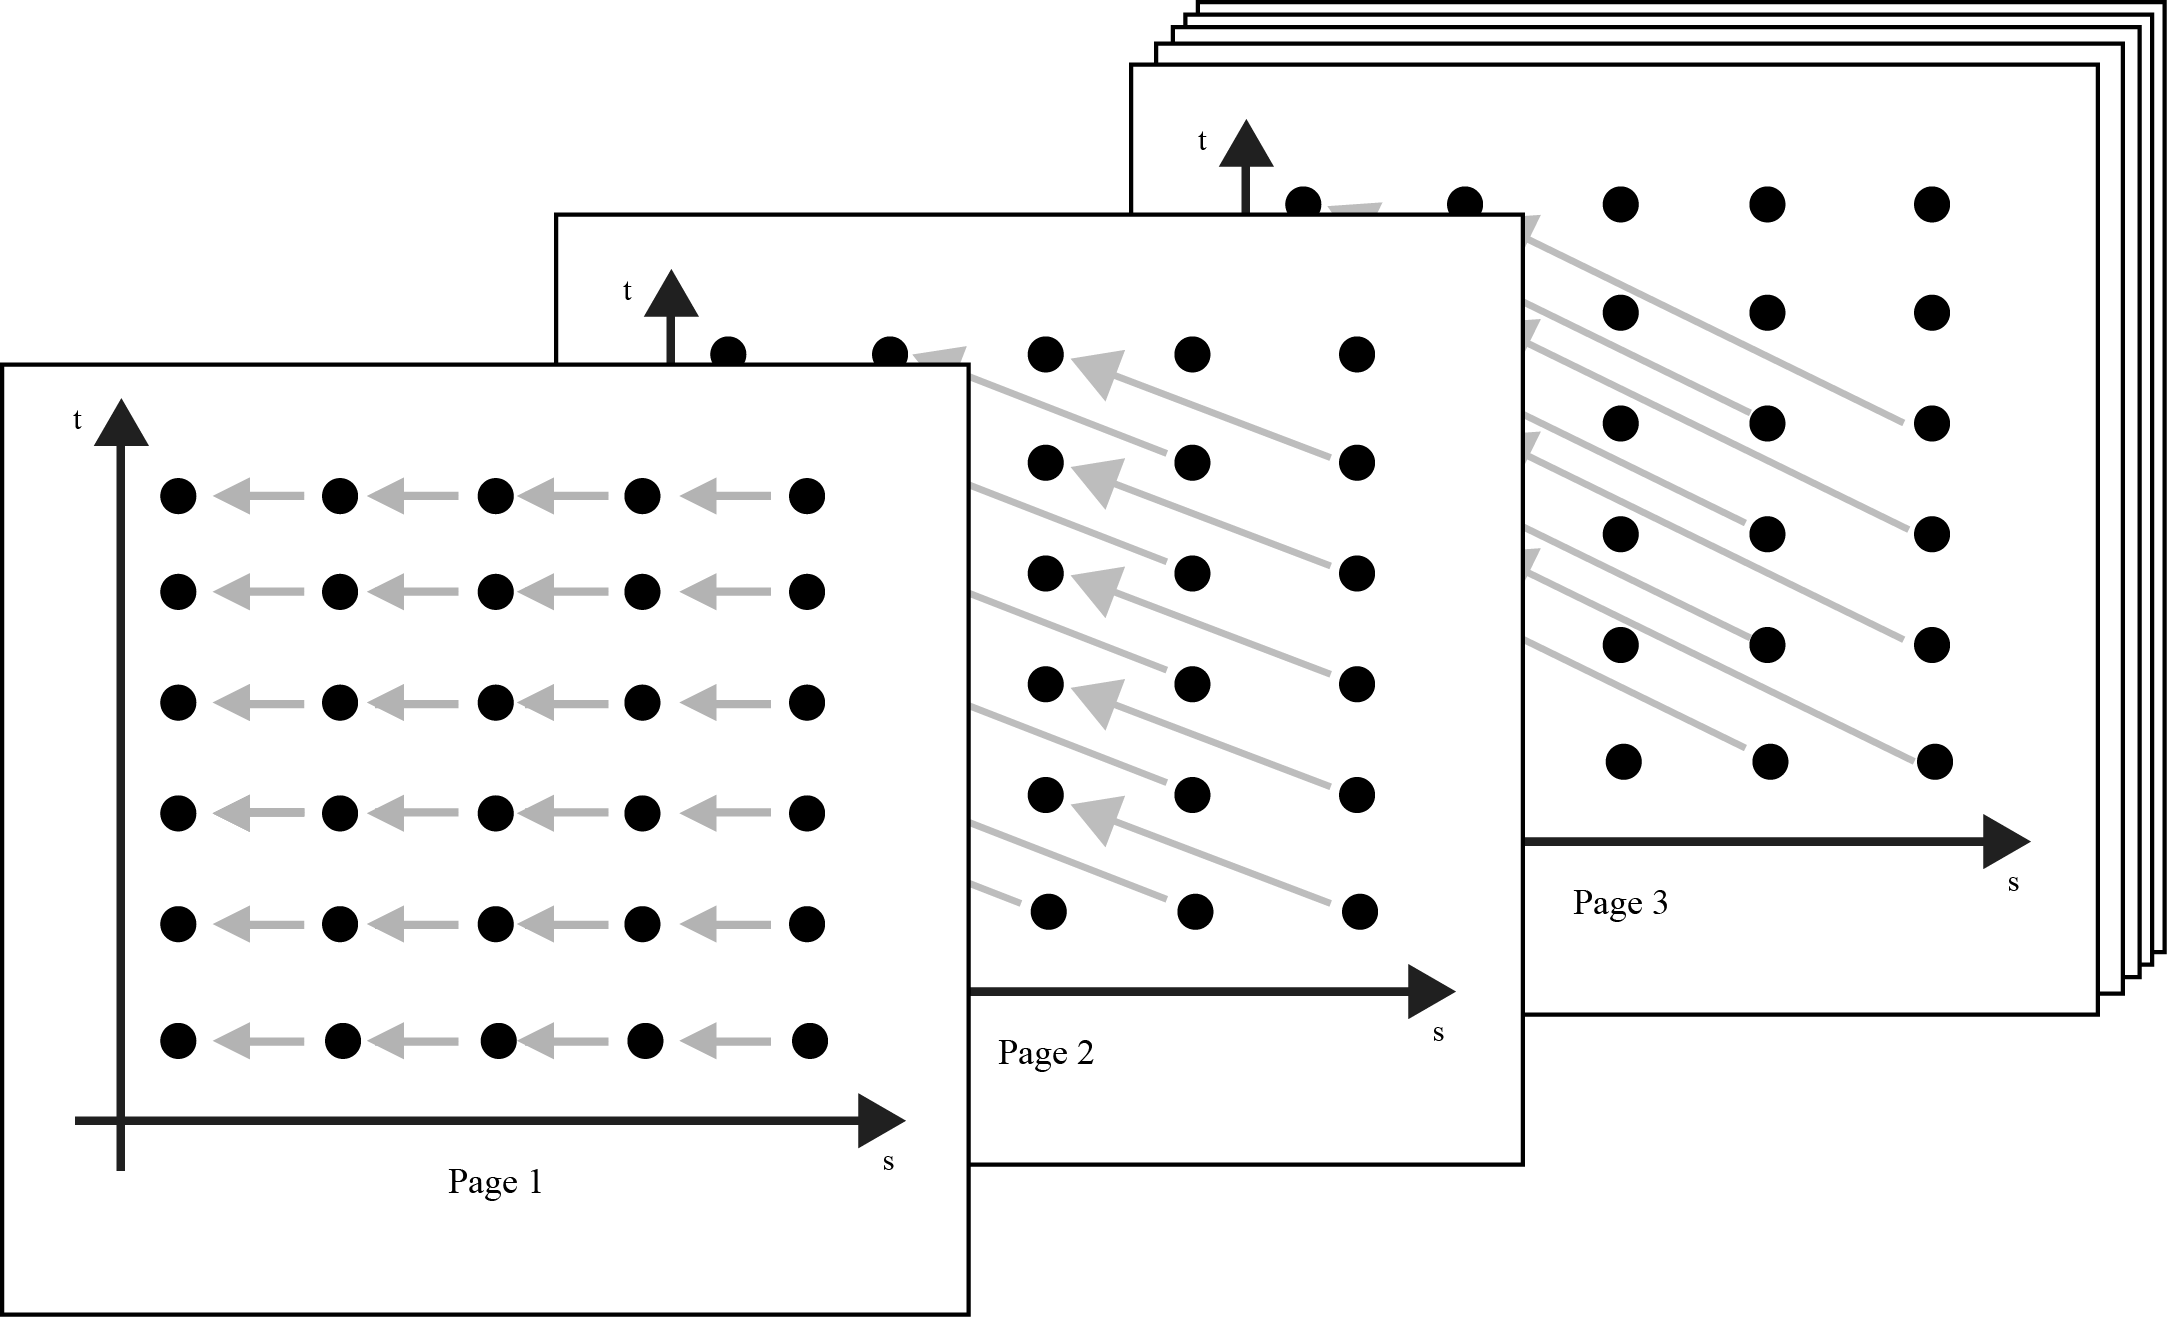
\includegraphics[width=\linewidth,height=0.5\textheight,keepaspectratio]{figures/cover.png}
  \end{center}
       \begin{minipage}{.35\linewidth}
    \begin{flushleft}
      \vspace{2em}
      {\fontsize{6pt}{2pt} \textit{Notes: These are notes live-tex'd
from a graduate course on Category O taught by Brian Boe at the
University of Georgia in Spring 2020. As such, any errors or
inaccuracies are almost certainly my own. } } \\
    \end{flushleft}
    \end{minipage}
    \hfill
    \begin{minipage}{.65\linewidth}
    \end{minipage}
  }







\begin{document}

\date{}
\maketitle
\begin{flushleft}
\textbf{D. Zack Garza} \\
\textit{University of Georgia} \\
\textit{dzackgarza@gmail.com} \\
{\tiny \textit{Last updated:} 2020-10-28 }
\end{flushleft}


\newpage
\tableofcontents

\hypertarget{definitions}{%
\section{Definitions}\label{definitions}}

\begin{itemize}
\tightlist
\item
  Indecomposable: doesn't decompose as \(A \oplus B\). Weaker than
  irreducible.
\item
  Irreducible: simple, i.e.~no nontrivial proper submodules. Implies
  indecomposable.
\item
  Completely reducible: Direct sum of irreducibles.
\item
  Solvable: Derived series terminates.
\item
  Borel: maximal solvable subalgebra.
\item
  Radical: Largest solvable ideal.
\item
  Semisimple: Direct sum of simple modules.

  \begin{itemize}
  \tightlist
  \item
    Acts in a diagonalizable way.
  \end{itemize}
\item
  Antidominant weight:
  \(\inner{\lambda + \rho}{\alpha\dual} \not\in\ZZ^{>0}\), equivalently
  \(M(\lambda) = L(\lambda)\).
\item
  Dominant weight:
  \(\inner{\lambda + \rho}{\alpha\dual} \not\in \ZZ^{< 0}\).
\item
  Regular weight: \(\lambda\) is regular iff the isotropy/stabilizer
  group
  \(\stab_W(\lambda) \definedas \theset{w\in W\suchthat w\lambda = w}= 1\),
  equivalently \(\abs{W\lambda} = \abs{W}\) so
  \(\inner{\lambda + \rho}{\alpha\dual} \neq 0\) for all
  \(\alpha\in \Phi\).
\item
  Singular weight: Not regular.
\item
  Linked: \(\mu \sim \lambda \iff \mu \in W\cdot \lambda\), the orbit of
  \(\lambda\) under \(W\), a.k.a. the linkage class of \(\lambda\).
\item
  Socle: Direct sum of all simple submodules.
\item
  Radical: Intersection of all maximal submodules, smallest submodule
  such that quotient is semisimple.
\item
  Head: \(M / \mathrm{rad}(M)\).
\end{itemize}

\hypertarget{list-of-notation}{%
\section{List of Notation}\label{list-of-notation}}

\begin{itemize}
\item
  \(M(\lambda)\): Verma Modules
\item
  \(L(\lambda)\): Unique simple \emph{quotient} of \(M(\lambda)\).
\item
  \(N(\lambda)\) the maximal \emph{submodule} of \(M(\lambda)\)
\item
  The root system
  \begin{align*}\Phi = \ts{\alpha \in \lieh\dual \suchthat [hx] = \alpha(h)x ~\forall h\in \lieh}\end{align*}
  containing roots \(\alpha\)

  \begin{itemize}
  \tightlist
  \item
    Abstractly: spans a Euclidean space,
    \(\lambda \alpha \in \phi \implies \lambda = \pm 1\), and closed
    under reflections about orthogonal hyperplanes.
  \end{itemize}
\item
  \(\Phi^+\) the corresponding positive system (choose a hyperplane not
  containing any root), \(\Phi \definedas \Phi^+ \disjoint \Phi^-\).
\item

  \begin{align*}s_\alpha(\wait) \definedas(\wait) - 2\inner{\wait}{\alpha} \frac{\alpha}{\norm{\alpha}^2}\end{align*}
  the corresponding reflection about the hyperplane \(H_\alpha\)
\item
  \(\lieg_\alpha \definedas \theset{x\in \lieg \suchthat [hx] = \alpha(h)x ~\forall h\in \lieh}\)
  the corresponding root space
\item
  The triangular decomposition
  \begin{align*}\lieg = \bigoplus_{\alpha\in \Phi^+} \lieg_{\alpha} \oplus \lieh \oplus \bigoplus_{\alpha \in \Phi^-} \lieg_{-\alpha} \definedas \lien^{-} \oplus \lieh \oplus \lien^{+}\end{align*}
\item
  \(\Delta\) the corresponding simple system of size \(\ell\), i.e
  \(\alpha = \sum_{\delta_k \in\Delta} c_\delta \delta_k\) with
  \(c_\delta \in \ZZ^{\geq 0}\).
\item
  \(\Lambda = \theset{\lambda \in E \suchthat \inner{\lambda}{\alpha\dual} \in \ZZ ~\forall \alpha\in\Phi }\)
  the integral weight lattice
\item
  \(\Lambda^+ = \ZZ^+\Omega\) the dominant integral weights

  \begin{itemize}
  \tightlist
  \item
    \(\Omega \definedas \theset{\bar \omega_1, \cdots, \bar \omega_\ell}\)
    the fundamental weights
  \end{itemize}
\item
  \([A: B]\) the composition factor multiplicity of \(B\) in a
  composition series for \(A\).
\item
  \((A: B)\) the composition factor multiplicity of \(B\) in a
  \emph{standard filtration} for \(A\).
\item
  \(\Phi_{[\lambda]} = \theset{\alpha\in \Phi \suchthat \inner{\lambda}{\alpha\dual} \in \ZZ}\)
  the integral root system of \(\lambda\)
\item
  \(\Delta_{[\lambda]}\) the corresponding simple system
\item
  \(W_{[\lambda]}\) the integral Weyl group of \(\lambda\)
\item
  \(\mu \uparrow \lambda\): strong linkage of weights
\item
  \(\OO_{\chi_\lambda}\): the block corresponding to \(\lambda\).
\item
  \(\ch M \definedas \sum_{\lambda \in \lieh\dual} \qty{\dim M_\lambda} e^{\lambda}\)
  the formal character.
\end{itemize}

\hypertarget{useful-facts}{%
\section{Useful Facts}\label{useful-facts}}

\begin{itemize}
\tightlist
\item
  \(\lambda\) dominant integral \(\implies w\lambda \leq \lambda\) for
  all \(W\).
\item
  \(M(\lambda)\) is simple \(\iff \lambda\) is antidominant.
\item
  The dot action is given by
  \(w\cdot \lambda = w(\lambda + \rho) - \rho\).
\item
  For any filtration
  \(0 \injects M^n \injects M^{n-1} \injects \cdots \injects M^1 \injects M^0 = M\),
  we have
  \begin{align*}\ch M = \sum_{i=1}^n \ch \qty{M^i/M^{i-1}},\end{align*}
  i.e.~the character of \(M\) is the sum of the characters of its
  composition factors (with multiplicity).
\item
  \(\hd(M(\lambda)) = L(\lambda)\)
\item
  \(\rad(M(\lambda)) = N(\lambda)\)
\item
  \(\soc(M(\lambda)) =_? M(w_0 \cdot \lambda) = L(\mu)\) for \(\mu\) the
  unique antidominant highest weight in the block determined by
  \(\lambda\) (?)
\item
  \(\soc(M(w \cdot \lambda)) = L(w_0 \cdot \lambda)\).
\item

  \begin{align*}[M(\lambda) : L(\mu)] \geq 1 \iff \mu \uparrow \lambda \qtext{(strong linkage)}\end{align*}
\end{itemize}

\hypertarget{sl2-theory}{%
\section{SL2 Theory}\label{sl2-theory}}

Definition The group and the algebra:

\begin{align*}
\liesl(n, \CC)     &= \theset{M \in \gl(n, \CC) \suchthat \det(M) = 1} \\
\liesl(n, \CC)  &= \theset{M \in \gl(n, \CC) \suchthat \tr(M) = 0}
.\end{align*}

\begin{itemize}
\tightlist
\item
  The usual representation on \(\CC^2\): \(h\) has eigenvalues
  \(\pm 1\), yields \(L(1)\).
\item
  The adjoint representation on \(\CC^3\):
  \(\ad h = \mathrm{diag}(2, 0, -2)\) with eigenvalues \(0, \pm 2\),
  yields \(L(2)\).
\end{itemize}

Generated by \begin{align*}
x =
\begin{bmatrix}
0 & 1 \\
0 & 0
\end{bmatrix}
,\quad
h =
\begin{bmatrix}
1 & 0 \\
0 & -1
\end{bmatrix}
,\quad
y =
\begin{bmatrix}
0 & 0 \\
1 & 0
\end{bmatrix}
\end{align*}

with relations

\begin{align*}
[hx] &= 2x \\
[hy] &= -2y \\
[xy] &= h \\
.\end{align*}

Some identifications: \begin{align*}
\Phi &= A_1 \\
\dim \lieh &= 1\\
\Lambda &\cong \ZZ \\
\Lambda_r & \cong \ZZ/2\ZZ \\
\Lambda^+ &= \theset{0, 1, 2, 3, \cdots} \\
W &= \theset{1, s_0} \quad \lambda \overset{s_0}\iff -\lambda \\
\chi_\lambda = \chi_\mu &\iff \mu = \lambda, -\lambda-2 \qtext{(linked)}\\
\Pi(M(\lambda)) &= \theset{\lambda, \lambda-2, \cdots} \\
\rho &= 1 \\
\alpha &= 2 \\
s_\alpha \cdot \lambda &= - \lambda - 2
.\end{align*}

For \(\lambda\) dominant integral \begin{align*}
N(\lambda) &\cong L(-\lambda - 2) \\
\dim L(\lambda) &= \lambda + 1 \\
\Pi(L(\lambda)) &= \theset{\lambda, \lambda-2, \cdots, -\lambda} \\
\dim \qty{L(\lambda)}_\mu &= 1 \quad\quad\forall \mu = \lambda-2i 
.\end{align*}

\begin{itemize}
\tightlist
\item
  Simple modules are parameterized by dominant integral weights:
  \begin{align*}M(\lambda) \text{ is simple } \iff \lambda \not\in\ZZ^{\geq 0} = \Lambda^+ \iff \dim L(\lambda) = \infty\end{align*}
\end{itemize}

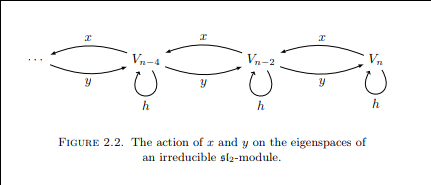
\includegraphics{figures/2020-03-16-13:59.png}\\

Finite-dimensional irreducible representations (i.e.~simple modules) of
\(\liesl(2, \CC)\) are in bijection with dominant integral weights
\(n\in \Lambda\), i.e.~\(n\in \ZZ^{\geq 0}\), are denoted \(M(n)\), and
each admits a basis \(\theset{\vector v_i\suchthat 0\leq i \leq n}\)
where \begin{align*}
h \cdot v_{i} &= (n-2 i) v_{i}\\
x \cdot v_{i} &= (n-i+1) v_{i-1}\\
y \cdot v_{i} &= (i+1)v_{i+1}
,\end{align*} setting \(v_{-1} = v_{n + 1}=0\) and letting \(v_0\) be
the unique vector in \(L(n)\) annihilated by \(x\).

\begin{itemize}
\tightlist
\item
  \(\mathrm{rad}~M(\lambda) = N(\lambda)\)
\item
  \(\mathrm{hd}~M(\lambda) = L(\lambda)\).
\item
  \(M(\lambda)\) for \(\lambda > 0\) not integral is simple, however
  \(-\lambda-2\not\in W\cdot \lambda\).
\item
  \(\lambda \geq 0 \implies \ch L(\lambda) = \ch M(\lambda) - \ch M(s_\alpha \cdot \lambda)\)
  where \(s_\alpha \cdot \lambda = -\lambda - 2\).
\item
  For \(\lambda \geq 0\), \(\dim L(\lambda) = \lambda + 1\) and so
  \begin{align*}\ch L(\lambda) = e^\lambda + e^{\lambda-2} + \cdots + e^{-\lambda} = {e^{\lambda + 1} - e^{\lambda - 1} \over e^1 - e^{-1}}.\end{align*}
\item
  For \(\lambda \neq \rho\in \ZZ\), the composition factors of
  \(M(\lambda)\) are \(M(\lambda), L(-\lambda - 2)\).
\item
  There is an exact sequence
\end{itemize}

\begin{center}
\begin{tikzcd}
0 \ar[r] \ar[equal]{d} & N(\lambda) \ar[r]\ar[equal]{d}  & M(\lambda) \ar[r]\ar[equal]{d}  & L(\lambda) \ar[r]\ar[equal]{d}  & 0\ar[equal]{d}  \\
0 \ar[r] & L(-\lambda-2) \ar[r] & M(\lambda) \ar[r] & L(\lambda) \ar[r] & 0
\end{tikzcd}
\end{center}

Characters: \begin{align*}
\ch M(\lambda) &= \ch L(\lambda) + \ch L(s_\alpha \cdot \lambda) \\
\ch M(s_\alpha \cdot \lambda) &= \ch L(s_\alpha \cdot \lambda)
.\end{align*}

We can think of this pictorially as the `head' on top of the socle:

\begin{align*}
M(\lambda) = \frac{L(\lambda)}{L(s_\alpha \cdot \lambda)}
.\end{align*}

We can invert the formula to get equation (2), which corresponds to
inverting this matrix:

\begin{align*}
\ch L(\lambda) &= \ch M(\lambda) - \ch M(s_\alpha \cdot \lambda) \\
\ch L(s_\alpha \cdot \lambda) &= \ch M(s_\alpha \cdot \lambda)
.\end{align*}

If \(\lambda \not\in\Lambda^+\), then
\(\ch L(\lambda) = \ch M(\lambda)\) and
\(b_{\lambda, 1} = 1, b_{\lambda, s_\alpha} = 0\) are again independent
of \(\lambda \in \lieh\dual \setminus \Lambda^+\).

\hypertarget{sl3}{%
\section{SL3}\label{sl3}}

\(\liesl(3, \CC)\) has root system \(A_2\):

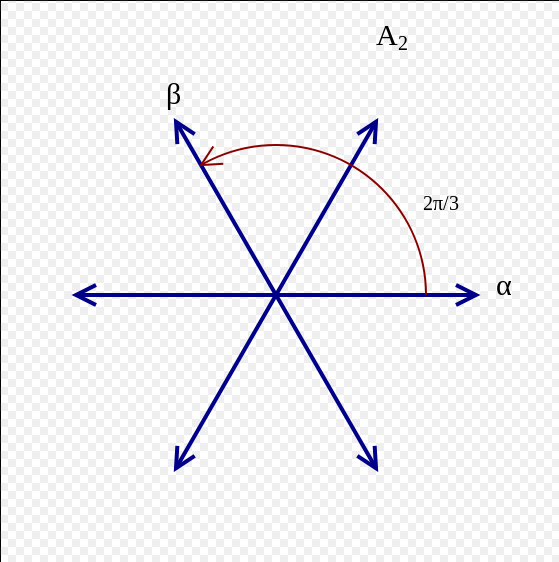
\includegraphics{figures/image_2020-05-01-16-37-30.png}\\

\begin{align*}
\Phi &= \theset{\pm \alpha, \pm \beta, \pm\gamma \definedas \alpha + \beta} \\
\Delta &= \theset{\alpha, \beta} \\
\Phi^+ &= \theset{\alpha, \beta, \gamma} \\
W &= \theset{1, s_\alpha, s_\beta, s_\alpha s_\beta, s_\beta s_\alpha, w_0 = s_\alpha s_\beta s_\alpha = s_\beta s_\alpha s_\beta}
.\end{align*}

For \(\lambda\) regular, integral, and antidominant:

\begin{itemize}
\tightlist
\item
  \(M(\lambda) = L(\lambda)\)
\item
  No other \(M(w\cdot \lambda)\) is simple
\item
  \(\soc(M(w\cdot \lambda)) = L(\lambda)\).
\item
  \([M(w\cdot \lambda) : L(\lambda)] = [M(w\cdot \lambda) : L(w\cdot \lambda)] = 1\)
  for all \(w\).
\item
  \(\ch L(s_\alpha \cdot \lambda) = \ch M(s_\alpha \cdot \lambda) - \ch M(\lambda)\).
\item
  \(\ch M(s_\alpha \cdot \lambda) = \ch L(s_\alpha \cdot \lambda) + \ch L(\lambda)\).
\item
  The Jantzen filtration when
  \(w \in \theset{s_{\alpha\beta}, s_{\beta\alpha}, w_0}\) is given by
  \begin{align*}
  M(w\cdot \lambda)^0 &= M(w\cdot \lambda) \\
  M(w\cdot \lambda)^1 &= ? \\
  M(w\cdot \lambda)^2 &= L(\lambda) \\
  M(w\cdot \lambda)^{\geq 3} &= 0
  .\end{align*}
\end{itemize}

\hypertarget{wednesday-january-8}{%
\section{Wednesday January 8}\label{wednesday-january-8}}

\begin{quote}
Course Website:
\url{https://faculty.franklin.uga.edu/brian/math-8030-spring-2020}
\end{quote}

\hypertarget{chapter-zero-review}{%
\subsection{Chapter Zero: Review}\label{chapter-zero-review}}

\begin{quote}
Material can be found in Humphreys 1972.
\end{quote}

\begin{exercise}[Assignment Zero]

Practice writing lowercase mathfrak characters!

\end{exercise}

In this course, we'll take \(k = \CC\).

\begin{definition}[Lie Algebra]

Recall that a Lie Algebra is a vector space \(\lieg\) with a bracket
\begin{align*}
[\wait, \wait]: \lieg\tensor \lieg \to \lieg
\end{align*} satisfying

\begin{itemize}
\item
  \([x x] = 0\) for all \(x\in \lieg\)
\item
  \([x [y z]] = [[x y] z] + [y [x z]]\) (The Jacobi identity)
\end{itemize}

\end{definition}

Note that the last axiom implies that \(x\) acts as a derivation.

\begin{exercise}[?]

Show that \([x y] = -[y x]\).

\begin{quote}
Hint: Consider \([x+y, x+y]\). Note that the converse holds iff
\(\ch k \neq 2\).
\end{quote}

\end{exercise}

\begin{exercise}[?]

Show that Lie Algebras never have an identity.

\end{exercise}

\begin{definition}[Abelian Lie Algebras]

\(\lieg\) is \emph{abelian} iff \([x y] = 0\) for all \(x,y\in\lieg\).

\end{definition}

There are also the usual notions (define for rings/algebras) of:

\begin{itemize}
\tightlist
\item
  Subalgebras,

  \begin{itemize}
  \tightlist
  \item
    A vector subspace that is closed under brackets.
  \end{itemize}
\item
  Homomorphisms

  \begin{itemize}
  \tightlist
  \item
    I.e. a linear transformation \(\phi\) that commutes with the
    bracket, i.e.~\(\phi([x y]) = [\phi(x) \phi(y)]\).
  \end{itemize}
\item
  Ideals
\end{itemize}

\begin{exercise}[?]

Given a vector space (possibly infinite-dimensional) over \(k\), then
(exercise) \(\liegl(V) \definedas \mathrm{End}_k(V)\) is a Lie algebra
when equipped with \([f g] = f\circ g - g\circ f\).

\end{exercise}

\begin{definition}[Representation]

A \emph{representation} of \(\lieg\) is a homomorphism
\(\phi: \lieg \to \gl(V)\) for some \(V\).

\end{definition}

\begin{example}[The adjoint representation]

The adjoint representation is
\begin{align*}  
\ad: \lieg &\to \liegl(\lieg) \\
\ad(x)(y) &\definedas [x y]
.\end{align*}

\end{example}

Representations give \(\lieg\) the structure of a module over \(V\),
where \(x\cdot v \definedas \phi(x)(v)\). All of the usual module axioms
hold, where now
\begin{align*}
[x y] \cdot v \da x\cdot(\cdot v) - y\cdot(x\cdot v)
\end{align*}

\begin{example}[?]

The trivial representation \(V = k\) where \(x\cdot a = 0\).

\end{example}

\begin{definition}[Irreducible]

\(V\) is \emph{irreducible} (or \emph{simple}) iff \(V\) as exactly two
\(\lieg\dash\)invariant subspaces, namely \(0, V\).

\end{definition}

\begin{definition}[Completely Reducible Modules]

\(V\) is \emph{completely reducible} iff \(V\) is a direct sum of simple
modules, and \emph{indecomposable} iff \(V\) can not be written as
\(V = M \oplus N\), a direct sum of proper submodules.

\end{definition}

There are several constructions for creating new modules from old ones:

\begin{itemize}
\item
  The \emph{contragradient/dual}:

  \begin{definition}[Contragradient dual]

  \begin{align*}
  V\dual &\definedas \hom_k(V, k) \qquad
  (x\cdot f) &= -f(x\cdot v)
  .\end{align*} for \(f\in V\dual, x\in \lieg, v\in V\).

  \end{definition}
\item
  The direct sum \(V\oplus W\) where
  \begin{align*}
  x\cdot(v, w) = (x\cdot v, x\cdot w)
  \end{align*}
\item
  The tensor product where
  \begin{align*}
  x\cdot(v\tensor w) = x\cdot v \tensor w + v\tensor x\cdot w
  \end{align*}
\item
  \(\hom_k(V, W)\) where
  \begin{align*}
  (x\cdot f)(v) = x\cdot f(v) - f(x\cdot v)
  \end{align*}

  \begin{itemize}
  \tightlist
  \item
    Note that if we take \(W=k\) then the first term vanishes and this
    recovers the dual.
  \end{itemize}
\end{itemize}

\hypertarget{semisimple-lie-algebras}{%
\subsection{Semisimple Lie Algebras}\label{semisimple-lie-algebras}}

\begin{definition}[Derived Ideal]

The \emph{derived ideal} is given by
\(\lieg^{(1)} \definedas [\lieg \lieg] \definedas \spanof_k\qty{\theset{[x y] \suchthat x,y\in\lieg }}\).

\end{definition}

This is the analog of the commutator subgroup.

\begin{lemma}[The derived ideal detects abelian algebras]

\(\lieg\) is abelian iff \(\lieg^{(1)} = \theset{0}\), and 1-dimensional
algebras are always abelian.

\end{lemma}

\begin{proof}[?]

This follows because if \([x y] \definedas xy = yx\) then
\([x y] = 0 \iff xy = yx\).

\end{proof}

\begin{definition}[Simple algebras]

A lie algebra \(\lieg\) is \emph{simple} iff the only ideals of
\(\lieg\) are \(0, \lieg\) and \(\lieg^{(1)} \neq \theset{0}\).

\end{definition}

Note that thus rules out the zero modules, abelian lie algebras, and
particularly 1-dimensional lie algebras.

\begin{definition}[Derived Series and Solvability]

The \emph{derived series} is defined by
\(\lieg^{(2)} = [\lieg^{(1)} \lieg^{(1)}]\), continuing inductively.
\(\lieg\) is said to be \textbf{solvable} if \(\lieg^{(n)} = 0\) for
some \(n\).

\end{definition}

\begin{lemma}[?]

Abelian implies solvable.

\end{lemma}

\begin{definition}[Nilpotent Algebras]

The \textbf{lower central series} of \(\lieg\) is defined as
\(\lieg_{j+1} \da [\lieg, \lieg_j]\). The lie algebra \(\lieg\) is
\textbf{nilpotent} if this series terminates at zero.

\end{definition}

\begin{remark}

Note that an \emph{element} \(x\) of a Lie algebra is nilpotent iff
\(\ad x\) is nilpotent as a matrix (so \(x\) is \emph{ad-nilpotent}),
i.e.~\(\ad(x)^n =0\) for some \(n\). There is a result, Engel's theorem,
which relates these two notions: a Lie algebra is nilpotent iff all of
its elements are nilpotent (with potentially different \(n\)s depending
on \(x\)).

\end{remark}

\begin{definition}[Semisimple]

\(\lieg\) is \emph{semisimple} (s.s.) iff \(\lieg\) has no nonzero
solvable ideals.

\end{definition}

\begin{exercise}[?]

Show that simple implies semisimple.

\end{exercise}

\begin{remark}

\envlist

\begin{enumerate}
\def\labelenumi{\arabic{enumi}.}
\tightlist
\item
  Semisimple algebras \(\lieg\) will usually have solvable subalgebras.
\item
  \(\lieg\) is semisimple iff \(\lieg\) has no nonzero abelian ideals.
\end{enumerate}

\end{remark}

\begin{definition}[Killing Form]

The \emph{Killing form} is given by
\(\kappa: \lieg \tensor \lieg \to k\) where
\(\kappa(x, y) = \tr(\ad x ~\ad y)\), which is a symmetric bilinear
form.

\end{definition}

\begin{lemma}[?]

\begin{align*}
\kappa([x y], z) = \kappa(x, [y z])
\end{align*}

\end{lemma}

\begin{definition}[Radical]

If \(\beta: V^{\tensor 2} \to k\) is any symmetric bilinear form, then
its radical is defined by

\begin{align*}
\rad \beta = \theset{v\in V \suchthat \beta(v, w) = 0 ~\forall w\in V}
.\end{align*}

\end{definition}

\begin{definition}[Nondegenerate Bilinear Forms]

A bilinear form \(\beta\) is \emph{nondegenerate} iff
\(\mathrm{rad}\beta = 0\).

\end{definition}

\begin{lemma}[?]

\(\mathrm{rad}\kappa \normal \lieg\) is an ideal, which follows by the
above associative property.

\end{lemma}

\begin{theorem}[Characterization of Semisimplicity Using the Killing Form]

\(\lieg\) is semisimple iff \(\kappa\) is nondegenerate.

\end{theorem}

\begin{example}[?]

The standard example of a semisimple lie algebra is

\begin{align*}
\lieg = \liesl(n, \CC) \definedas \theset{x\in \liegl(n, \CC) \suchthat \tr(x) = 0 }
\end{align*}

\end{example}

\begin{remark}

From now on, \(\lieg\) will denote a semisimple lie algebra over
\(\CC\).

\end{remark}

\begin{theorem}[Weyl's Complete Reducibility Criterion]

Every finite dimensional representation of a semisimple \(\lieg\) is
completely reducible.

\end{theorem}

In other words, the category of finite-dimensional representations is
relatively uninteresting -- there are no extensions, so everything is a
direct sum. Thus once you classify the simple algebras (which isn't
terribly difficult), you have complete information.

\hypertarget{friday-january-10th}{%
\section{Friday January 10th}\label{friday-january-10th}}

\hypertarget{root-space-decomposition}{%
\subsection{Root Space Decomposition}\label{root-space-decomposition}}

Let \(\lieg\) be a finite dimensional semisimple lie algebra over
\(\CC\). Recall that this means it has no proper solvable ideals. A more
useful characterization is that the Killing form
\(\kappa: \lieg\tensor \lieg \to \lieg\) is a \emph{non-degenerate}
symmetric (associative) bilinear form. The running example we'll use is
\(\lieg = \liesl(n, \CC)\), the trace zero \(n\times n\) matrices. Let
\(\lieh\) be a maximal toral subalgebra, where \(x\in\lieg\) is
\emph{toral} if \(x\) is semisimple, i.e.~\(\ad x\) is semisimple
(i.e.~diagonalizable).

\begin{example}[?]

\(\lieh\) is the diagonal matrices in \(\liesl(n, \CC)\).

\end{example}

\begin{remark}

\(\lieh\) is abelian, so \(\ad \lieh\) consists of commuting semisimple
elements, which (theorem from linear algebra) can be simultaneously
diagonalized.

\end{remark}

\begin{definition}[Root Space Decomposition]

This leads to the root space decomposition,

\begin{align*}
\lieg = \lieh \oplus \bigoplus_{\alpha\in \Phi} \lieg_\alpha
.\end{align*}

where
\begin{align*}
\lieg_\alpha = \theset{x\in \lieg \suchthat [h x] = \alpha(h) x ~\forall h\in \lieh}
\end{align*} where \(\alpha \in \lieh\dual\) is a linear functional.

\end{definition}

Here \(\lieh = C_\lieg(\lieh)\), so \([h x] = 0\) corresponds to zero
eigenvalues, and (fact) it turns out that \(\lieh\) is its own
centralizer.

\begin{definition}[Root System]

We then obtain a set of roots of \(\lieh, \lieg\) given by
\begin{align*}
\Phi = \theset{\alpha\in\lieh\dual \suchthat \alpha\neq 0, \lieg_\alpha \neq \theset{0}}
\end{align*}

\end{definition}

\begin{example}[?]

\(\lieg_\alpha = \CC E_{ij}\) for some \(i\neq j\), the matrix with a 1
in the \(i,j\) position and zero elsewhere.

\end{example}

\begin{remark}

The restriction \(\restrictionof{\kappa}{\lieh}\) is nondegenerate, so
we can identify \(\lieh, \lieh\dual\) via \(\kappa\) (can always do this
with vector spaces with a nondegenerate bilinear form), where \(\kappa\)
maps to another bilinear form \((\wait, \wait)\). We thus get a
correspondence
\begin{align*}
\lieh\dual \ni \lambda \iff t_\lambda \in \lieh \\
\lambda(h) = \kappa(t_\lambda, h) \quad\text{where } (\lambda, \mu) = \kappa(t_\lambda, t_\mu)
.\end{align*}

\end{remark}

\hypertarget{facts-about-phi-and-root-spaces}{%
\subsection{\texorpdfstring{Facts About \(\Phi\) and Root
Spaces}{Facts About \textbackslash Phi and Root Spaces}}\label{facts-about-phi-and-root-spaces}}

\begin{definition}[Abstract Root System]

Let \(\alpha, \beta \in \Phi\) be roots.

\begin{enumerate}
\def\labelenumi{\arabic{enumi}.}
\item
  \(\Phi\) spans \(\lieh\dual\) and does not contain zero.
\item
  If \(\alpha \in \Phi\) then \(-\alpha \in \Phi\), but no other scalar
  multiple of \(\alpha\) is in \(\Phi\).

  \begin{itemize}
  \tightlist
  \item
    Note: see \cref{rmk:aside1}.
  \end{itemize}
\item
  \((\beta, \alpha\dual) \in \ZZ\)
\item
  \(s_\alpha(\beta) \definedas \beta - (\beta, \alpha\dual)\alpha \in \Phi\).

  \begin{itemize}
  \tightlist
  \item
    Note: see \cref{rmk:aside2}
  \end{itemize}
\end{enumerate}

\end{definition}

\begin{remark}

\label{rmk:aside1} An aside:

\begin{itemize}
\item
  \(\dim \lieg_\alpha = 1\).
\item
  If \(0 \neq x_\alpha \in \lieg_\alpha\) then there exists a unique
  \(y_\alpha \in \lieg_{-\alpha}\) such that
  \(x_\alpha, y_\alpha, h_\alpha \definedas [x_\alpha, y_\alpha]\) spans
  a 3-dimensional subalgebra in \(\liesl_2\), given by
  \begin{align*}
  x_\alpha = 
  \begin{bmatrix}
  0 & 1 \\
  0 & 0
  \end{bmatrix}, 
  \quad
  y_\alpha = 
  \begin{bmatrix}
  0 & 0 \\
  1 & 0
  \end{bmatrix},
  \quad
  h_\alpha =\begin{bmatrix}
  1 & 0 \\
  0 & -1
  \end{bmatrix}
  .\end{align*}
\item
  Under the correspondence \(\lieh \iff \lieh\dual\) induced by
  \(\kappa\),
  \begin{align*}
  h_\alpha \iff \alpha\dual \definedas \frac{2\alpha}{(\alpha, \alpha)}
  \end{align*} Thus for all \(\lambda \in\lieh\dual\),
  \begin{align*}
  \lambda(h_\alpha) = (\lambda, \alpha\dual) = \frac{2(\lambda, \alpha)}{(\alpha, \alpha)}
  .\end{align*}
\item
  If \(\alpha + \beta \neq 0\), then \(\kappa(g_\alpha, g_\beta) = 0\).
\end{itemize}

\end{remark}

\begin{remark}

\label{rmk:aside2} If \(\alpha + \beta \in \Phi\), then
\([\lieg_\alpha \lieg_\beta] = \lieg_{\alpha+\beta}\).

\begin{example}[?]

Example: If \(\alpha = E_{ij}, \beta = E_{jk}\) where \(k\neq i\), then
\([E_{ij}, E_{jk}]= E_{ik}\).

\end{example}

\begin{itemize}
\tightlist
\item
  \(\lieg\) is generated as an algebra by the root spaces
  \(\lieg_\alpha\)
\item
  Root strings: If \(\beta \neq \pm\alpha\), then the roots of the form
  \(\alpha + k\beta\) for \(k\in \ZZ\) form an unbroken string
  \begin{align*}
  \alpha - r\beta, \cdots, \alpha-\beta, \alpha,\alpha+\beta,\cdots,\alpha + \ell \beta
  \end{align*} consisting of at most 4 roots where
  \(r-s = (\alpha, \beta\dual)\).
\end{itemize}

\end{remark}

\begin{example}[?]

The circled roots below form the root string for \(\beta\):

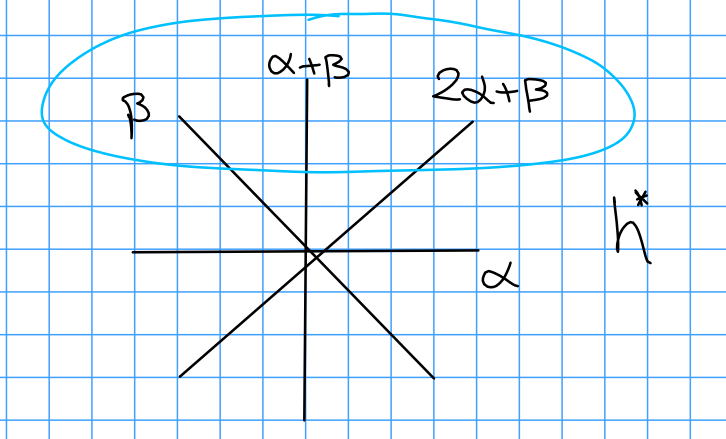
\includegraphics{figures/2020-01-10-09:34.png}\\

In general, a subset \(\Phi\) of a real euclidean space \(E\) satisfying
conditions (1) through (4) is an \emph{(abstract) root system}. Note
that when \(\Phi\) comes from a \(\lieg\), we define
\(E\definedas \RR \Phi\).

\end{example}

\hypertarget{the-root-system}{%
\subsubsection{The Root System}\label{the-root-system}}

\begin{definition}[Simple System]

There exists a subset \(\Delta \subseteq \Phi\) such that

\begin{itemize}
\tightlist
\item
  \(\Delta\) is a \(\CC\dash\)basis for \(\lieg\dual\)
\item
  \(\beta\in\Phi\) implies that
  \(\beta = \sum_{\alpha \in \Delta} c_\alpha \alpha\) with either

  \begin{itemize}
  \tightlist
  \item
    All \(c_\alpha \in \ZZ_{\geq 0} \iff \beta \in \Phi^+\) or
    \(\beta < 0\).
  \item
    All \(c_\alpha \in \ZZ_{\leq 0} \iff \beta \in \Phi^-\) or
    \(\beta > 0\).
  \end{itemize}
\end{itemize}

\(\Delta\) is called a \textbf{simple system}.

\end{definition}

\begin{definition}[Positive Roots, Height]

If \(\Delta = \theset{a_1, \cdots, a_\ell}\) then \(\Phi^+\) are the
\emph{positive roots}, and if
\(\Phi^+ \ni \beta = \sum_{\alpha \in \Delta} c_\alpha \alpha\), then
the \emph{height} of \(\beta\) is defined as

\begin{align*}
\height(\beta) \da 
\sum c_\alpha \in \ZZ_{> 0}
\end{align*}

\end{definition}

\begin{definition}[Root Lattice, Dual Root System]

Note that \(\ZZ \Phi \definedas \Lambda_r\) is a lattice, and is
referred to as the \emph{root lattice}, and
\(\Lambda_r \subset E = \RR \Phi\).

We also have
\begin{align*}
\Phi^+ = \theset{\beta\dual \suchthat \beta \in \Phi}
,\end{align*} the \emph{dual root system}, is a root system with simple
system \(\Delta\dual\).

\end{definition}

\begin{proposition}[Important subalgebras of a Lie algebra]

\begin{align*}  
\lien = \lien^+ &\da \sum_{\beta > 0} \lieg_\beta
&& \text{Upper triangular with zero diagonal,} \\
\lien^- &\da \sum_{\beta > 0} \lieg_{-\beta}
&& \text{Lower triangular with zero diagonal,} \\
\lieb &\da \lieh + \lien
&& \text{Upper triangular (the "Borel" subalgebra),} \\
\lieb^- &\da \lieh + \lien^-
&& \text{Lower triangular.} 
.\end{align*}

\end{proposition}

\begin{definition}[Triangular/Cartan Decomposition]

\begin{align*}
\lieg = \lien^- \oplus \lieh \oplus \lien
\end{align*}

\end{definition}

\begin{fact}

If \(\beta \in \Phi^+\setminus \Delta\), and if \(\alpha \in \Delta\)
such that \((\beta, \alpha\dual) > 0\), then
\(\beta - (\beta,\alpha\dual)\alpha \in \Phi^+\) has height strictly
less than the height of \(\beta\).

\end{fact}

\begin{remark}

By root strings, \(\beta-\alpha\in\Phi^+\) is positive root of height
one less than \(\beta\), yielding a way to induct on heights (useful
technique).

\end{remark}

\hypertarget{weyl-groups}{%
\subsubsection{Weyl Groups}\label{weyl-groups}}

For \(\alpha \in \Phi\), define

\begin{align*}
S_\alpha : \lieh\dual &\to \lieh\dual \\
\lambda &\mapsto \lambda - (\lambda, \alpha\dual)\alpha
.\end{align*}

This is reflection in the hyperplane in \(E\) perpendicular to
\(\alpha\):

\begin{figure}
\centering
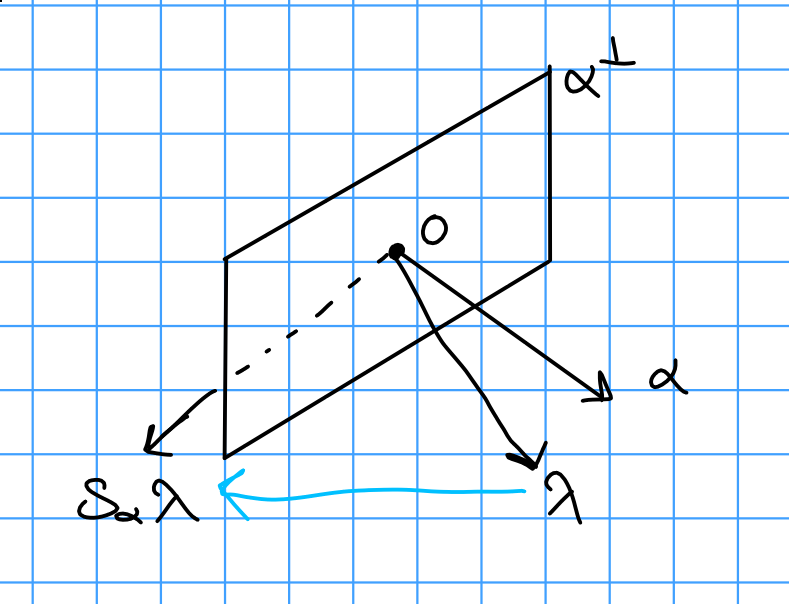
\includegraphics[width=3.64583in,height=\textheight]{figures/2020-01-10-09:51.png}
\caption{Reflection through a hyperplane}
\end{figure}

Note that \(s_\alpha^2 = \id\).

\begin{definition}[Weyl Group]

Define \(W\) as the subgroup of \(\gl(E)\) generated by all \(s_\alpha\)
for \(\alpha \in \Phi\), this is the \emph{Weyl group} of \(\lieg\) or
\(\Phi\), which is finite and
\(W = \generators{s_\alpha \suchthat \alpha\in\Delta}\) is generated by
simple reflections.

\end{definition}

By (4), \(W\) leaves \(\Phi\) invariant. In fact \(W\) is a finite
Coxeter group with generators
\(S = \theset{s_\alpha \suchthat \alpha\in \Delta}\) and defining
relations \((s_\alpha s_\beta)^{m(\alpha, \beta)} = 1\) for
\(\alpha,\beta \in \Delta\) where
\(m(\alpha, \beta) \in \theset{2,3,4,6}\) when \(\alpha \neq \beta\) and
\(m(\alpha, \alpha) = 1\).

\begin{definition}[Crystallographic group]

If this finiteness on numerical conditions are met, then \(W\) is
referred to as a \emph{Crystallographic group}.

\end{definition}

\hypertarget{monday-january-13th}{%
\section{Monday January 13th}\label{monday-january-13th}}

\hypertarget{lengths}{%
\subsection{Lengths}\label{lengths}}

Recall that we have a root space decomposition
\(\lieg = \lieh \oplus \bigoplus_{\beta \in \Phi} \lieg_\beta\) for
finite dimensional semisimple lie algebras over \(\CC\). We have
\(s_\beta(\lambda) = \lambda - (\lambda, \beta\dual)\beta\), for
\(\lambda \in \lieh\dual\) and the Weyl group
\begin{align*}
W = \generators{s_\beta \suchthat \beta\in\Phi} = \generators{s_\alpha \suchthat \alpha \in \Delta}
\end{align*} where \(\Delta = \theset{a_i}\) are the simple roots.

For \(w\in W\), we can take the reduced expression for \(w\) by writing
\(w = s_1 \cdots s_n\) with \(s_i\) simple and \(n\) minimal. The length
is uniquely determined, but not the expression. So we define
\(\ell(w) \definedas n\) where \(\ell(1) \definedas 0\).

\begin{fact}

\envlist

\begin{enumerate}
\def\labelenumi{\arabic{enumi}.}
\item
  \(\ell(w)\) is the size of the set
  \(\theset{\beta\in\Phi^+ \suchthat w\beta < 0}\)

  \begin{itemize}
  \tightlist
  \item
    The above set is equal to \(\Phi^+ \intersect w\inv \Phi^-\).
  \item
    In particular, for \(\beta \in \Phi^+\), \(\beta\) is simple
    (i.e.~\(\beta \ni \Delta\) iff \(\ell(s_\beta) = 1)\).
  \item
    Note: \(\alpha\) is the only root that \(s_\alpha\) sends to a
    negative root, so \(s_\alpha(\beta) > 0\) for all
    \(\beta\in\Phi^+\setminus\theset{\alpha}\).
  \end{itemize}
\item
  \(\ell(w) = \ell(w\inv)\) for all \(w\in W\), so \(\ell(w)\) is also
  the size of \(\Phi \intersect w\Phi\) (replacing \(w\inv\) with \(w\))
\item
  There exists a unique \(w_0 \in W\) with \(\ell(w_0)\) maximal such
  that \(\ell(w_0) = \abs{\Phi^+}\) and \(w_0(\Phi^+) = \Phi^-\).

  \begin{itemize}
  \tightlist
  \item
    Also \(\ell(w_0 w) = \ell(w_0) - \ell(w)\) \footnote{Note that the
      product of reduced expressions is not usually reduced, so the
      length isn't additive.}
  \end{itemize}
\item
  For \(\alpha \in \Phi^+\), \(w\in W\), we have either
\end{enumerate}

\begin{align*}
\ell(w s_\alpha) > \ell (w) \iff w(\alpha) > 0 \\
\ell(w s_\alpha) < \ell (w) \iff w(\alpha) < 0 \\
.\end{align*}

Taking inverses yields
\(\ell(s_\alpha w) > \ell(w) \iff w\inv\alpha > 0\).

\end{fact}

\hypertarget{bruhat-order}{%
\subsection{Bruhat Order}\label{bruhat-order}}

\begin{definition}[Bruhat Order]

Let \(S\) be the set of simple reflections,
i.e.~\(S = \theset{s_\alpha \suchthat \alpha \in \Delta}\). Then define
\begin{align*}
T \definedas \Union_{w\in W} wSw\inv = \theset{s_\beta \suchthat \beta\in\Phi^+}
.\end{align*} This is the set of \emph{all} reflections in \(W\) through
hyperplanes in \(E\).

We'll write \(w' \mapsvia{t} w\) means \(w=tw'\) and
\(\ell(w') < \ell(w)\). Note that in the literature, it's also often
assumed that that \(\ell(w') = \ell(w) - 1\). In this case, we say
\(w'\) \textbf{covers} \(w\), and refer to this as \textbf{the covering
relation}. So \(w' \to w\) means that \(w' \mapsvia{t} w\) for some
\(t\in T\). We extend this to a partial order: \(w' < w\) means that
there exists a \(w\) such that
\begin{align*}
w' = w_0 \to w_1 \to \cdots \to w_n = w.
\end{align*} This is called the \textbf{Bruhat-Chevalley order} on
\(W\).

\end{definition}

\begin{corollary}[?]

\(w' < w \implies \ell(w') < \ell(w)\), so \(1\in W\) is the unique
minimal element in \(W\) under this order.

\end{corollary}

It turns out that if we set \(w = w' t\) instead, this results in the
same partial order. If you restrict \(T\) to simple reflections, this
yields the \textbf{weak Bruhat order} In this case, the left and right
versions differ, yielding the \textbf{left/right weak Bruhat orders}
respectively. \footnote{Note that this is because conjugating a simple
  reflection may not yield a simple reflection again.}

Recall that lie algebras yield finite crystallographic coxeter groups.

\begin{proposition}[Properties of the Bruhat Order]

For \((W, S)\) a coxeter group,

\begin{enumerate}
\def\labelenumi{\alph{enumi}.}
\tightlist
\item
  \(w' \leq w\) iff \(w'\) occurs as a subexpression/subword of every
  reduced expression \(s_1 \cdots s_n\) for \(w\), where a subexpression
  is any subcollection of \(s_i\) in the same order.\footnote{Note that
    this implies that \(1\) is not only a minimal element in this order,
    but an infimum.}
\end{enumerate}

\begin{enumerate}
\def\labelenumi{\alph{enumi}.}
\setcounter{enumi}{1}
\item
  Adjacent elements \(w', w\) (i.e.~\(w' < w\) and there does not exist
  a \(w''\) such that \(w' < w'' < w\)) in the Bruhat order differ in
  length by 1.
\item
  If \(w' < w\) and \(s\in S\), then \(w' s \leq w\) or \(w's \leq ws\)
  (or both). i.e., if \(\ell(w_1) = 2 = \ell(w_2)\), then the size of
  \(\theset{w\in W \suchthat w_1 < w < w_2}\) is either 0 or 2.
\end{enumerate}

\begin{tikzpicture}
    \node (0) at (0, 2) [label=$w_2$]{};
    \node (1) at (2, 0) {};
    \node (2) at (-2, 0) {};
    \node (3) at (0, -2) [label=below:$w_1$]{};
    \draw (0.center) to (2.center);
    \draw (2.center) to (3.center);
    \draw (0.center) to (1.center);
    \draw (1.center) to (3.center);
\end{tikzpicture}

\end{proposition}

\hypertarget{properties-of-universal-enveloping-algebras}{%
\subsection{Properties of Universal Enveloping
Algebras}\label{properties-of-universal-enveloping-algebras}}

Let \(\lieg\) be any lie algebra, and \(\phi: \lieg \to A\) be any map
into an associative algebra. Then there exists an object \(U(\lieg)\)
and a map \(i\) such that the following diagram commutes:

\begin{center}\includesvg[width=0.7\linewidth]{4bec7819a76ef6f1d25aff3c87426d0382104591}\end{center}

where \(\tilde \phi\) is a map in the category of associative algebras.

Moreover any lie algebra homomorphism \(\lieg_1 \to \lieg_1\) induces a
morphism of associative algebras \(U(\lieg_1) \to U(\lieg_2)\), where
\(\lieg\) generates \(U(\lieg)\) as an algebra.

\(U(\lieg)\) can be constructed as
\begin{align*}
U(\lieg) = T(\lieg)/ \generators{ [x,y] - x\tensor y - y\tensor x \suchthat x,y\in\lieg}
.\end{align*} Note that this ideal is not necessarily homogeneous.

\begin{proposition}[Properties of the Universal Enveloping Algebra]

\envlist

\begin{itemize}
\tightlist
\item
  Usually noncommutative
\item
  Left and right Noetherian
\item
  No zero divisors
\item
  \(\lieg \actson U(\lieg)\) by the extension of the adjoint action,
  \((\ad x)(u) = xu - ux\) for \(x\in \lieg, u\in U(\lieg)\).
\end{itemize}

\end{proposition}

\begin{theorem}[Poincaré-Birkhoff-Witt (PBW]

If \(\theset{x_1, \cdots x_n}\) is a basis for \(\lieg\), then
\(\theset{x_1^{t_1}, \cdots, x_n^{t_n} \suchthat t_i \in \ZZ^+}\)
(noting that \(x^n = x\tensor x \tensor \cdots x\) and \(\ZZ^+\)
includes 0) is a basis for \(U(\lieg)\).

\end{theorem}

\begin{corollary}[?]

\(i:\lieg \to U(\lieg)\) is injective, so we can think of
\(\lieg \subseteq U(\lieg)\). If \(\lieg\) is semisimple, then it admits
a triangular decomposition \(\lieg = \lien^- \oplus \lieh \oplus \lien\)
and choosing a compatible basis for \(\lieg\) yields
\(U(\lieg) = U(\lien^-)\tensor U(\lieh) \tensor U(\lien)\).

If \(\phi: \lieg \to \gl(V)\) is any Lie algebra representation, it
induces an algebra representation \(U(\lieg)\) of \(U(\lieg)\) on \(V\)
and vice-versa. It satisfies
\begin{align*}x\cdot (y \cdot v) - y\cdot (x \cdot v) = [x y] \cdot v\end{align*}
for all \(x,y \in \lieg\) and \(v\in V\).

\end{corollary}

\begin{remark}

Note that this lets us go back and forth between Lie algebra
representations and associative algebra representations, i.e.~the theory
of modules over rings.

\end{remark}

\begin{remark}

A note on notation: \(\mathcal Z(\lieg)\) denotes the center of
\(U(\lieg)\).

\end{remark}

\hypertarget{integral-weights}{%
\subsection{Integral Weights}\label{integral-weights}}

We have a Euclidean space \(E = \RR \Phi^+\), the \(\RR\dash\)span of
the roots.

\begin{definition}[Integral Weight Lattice]

We also have the \textbf{integral weight lattice}
\begin{align*}
\Lambda = \theset{\lambda \in E \suchthat (\lambda, \alpha\dual) \in \ZZ ~\forall \alpha\in\Phi (\text{or}~ \Phi^+ ~\text{or}~ \Delta)}
.\end{align*}

\end{definition}

\begin{definition}[Ordering of Weights]

There is a sublattice \(\Lambda_r \subseteq \Lambda\), which is an
additive subgroup of finite index. There is a partial order of
\(\Lambda\) on \(E\) and \(\lieh\dual\). We write
\begin{align*}
\mu \leq \lambda \iff \lambda - \mu \in \ZZ^+ \Delta = \ZZ^+ \Phi^+
\end{align*}

\end{definition}

\begin{definition}[Dominant Integral Weights]

For a basis \(\Delta = \theset{\alpha_1, \cdots, \alpha_n}\), define a
dual basis \((w_i ,\alpha_j\dual) = \delta_{ij}\). The fundamental
weights are given by a \(\ZZ\dash\)basis for \(\Lambda\). Then
\(\Lambda\) is a free abelian group of rank \(\ell\), and
\begin{align*}
\Lambda^+ = \ZZ^+ w_1 + \cdots + \ZZ^+ w_\ell
\end{align*} are the \textbf{dominant integer weights}.\footnote{Note
  that in Jantzen's book, \(X\) is used for \(\Lambda\) and \(X^+\)
  correspondingly.}

\end{definition}

\hypertarget{wednesday-january-15th}{%
\section{Wednesday January 15th}\label{wednesday-january-15th}}

\hypertarget{review}{%
\subsection{Review}\label{review}}

\begin{definition}[Weyl Vector]

The Weyl vector is given by
\begin{align*}
\rho = \bar \omega_1 + \cdots + \bar \omega_\ell = \frac 1 2 \sum_{\beta \in \Phi^+} \beta \in \Lambda^+
.\end{align*}

\end{definition}

\begin{proposition}[Properties of the Weyl vector]

envlist - If \(\alpha \in \Delta\) then \((\rho, \alpha\dual) = 1\) -
\(s_\alpha(\rho) = \rho - \alpha\).

\end{proposition}

\begin{fact}

Let \(\lambda \in \Lambda^+\); a few facts:

\begin{enumerate}
\def\labelenumi{\arabic{enumi}.}
\tightlist
\item
  The size of \(\theset{\mu\in \Lambda^+ \suchthat \mu \leq \lambda}\)
  (with the partial order from last time) is finite.
\item
  \(w\lambda < \lambda\) for all \(w\in W\).
\end{enumerate}

\end{fact}

\begin{definition}[Weyl Chamber]

The \textbf{Weyl chamber} for a fixed root in \(E\) a Euclidean space is
\begin{align*}
C = \theset{\lambda \in E \suchthat (\lambda, \alpha) > 0 ~ \forall \alpha\in\Delta}
\end{align*}

\end{definition}

\begin{remark}

Note that the hyperplane splits \(E\) into connected components, we mark
this component as distinguished.

\begin{itemize}
\tightlist
\item
  A connected component of the union of hyperplanes is orthogonal to
  roots.
\item
  They're in bijection with \(\Delta\).
\item
  They're permuted simply transitively by \(W\).
\end{itemize}

We also let \(\bar C\) denote the \textbf{fundamental domain}.

\end{remark}

\hypertarget{weight-representations}{%
\subsection{Weight Representations}\label{weight-representations}}

\begin{definition}[Weights, Weight Spaces, and Multiplicities]

For \(\lambda \in \lieh\dual\), we let
\begin{align*}  
M_\lambda \da
\theset{v\in M \suchthat h\cdot v = \lambda(h) v ~\forall h\in\lieh}
.\end{align*} denote a \textbf{weight space} of \(M\) if
\(M_\lambda \neq 0\). In this case, \(\lambda\) is a \textbf{weight} of
\(M\). The dimension of \(M_\lambda\) is the \textbf{multiplicity} of
\(\lambda\) in \(M\), and we define the set of weights as
\begin{align*}  
\Pi(M) \da
\theset{\lambda \in \lieh\dual \suchthat M_\lambda \neq 0}
.\end{align*}

\end{definition}

\begin{example}[?]

If \(M = \lieg\) under the adjoint action, then
\(\Pi(M) = \Phi \union \theset{0}\).

\end{example}

\begin{remark}

The weight vectors for distinct weights are linearly independent. Thus
there is a \(\lieg\dash\)submodule given by \(\sum_\lambda M_\lambda\),
which is in fact a direct sum. It may not be the case that
\(\sum_\lambda M_\lambda = M\), and can in fact be zero, although this
is an odd situation. \footnote{See Humphreys \#1, \#20.2, p.~110.} In
our case, we'll have a \emph{weight module}
\(M = \bigoplus_\lambda M_\lambda\), where \(\lieh\actson M\)
semisimply.

\end{remark}

\hypertarget{finite-dimensional-modules}{%
\subsection{Finite Dimensional
Modules}\label{finite-dimensional-modules}}

Recall \textbf{Weyl's complete reducibility theorem}, which implies that
any finite dimensional \(\lieg\dash\)module is a weight module. In fact,
\(\lien, \lien^- \actson M\) nilpotently.

\begin{fact}

\envlist

\begin{itemize}
\tightlist
\item
  \(\Pi(M) \subset \Lambda\) is a subset of the integral lattice.
\item
  \(\Pi(M)\) is \(W\dash\)invariant.
\item
  \(\dim M_\lambda = \dim M_{w\lambda}\) for any
  \(\lambda \in \Pi(M), w\in W\).
\end{itemize}

\end{fact}

\hypertarget{simple-finite-dimensional-liesl2-ccdashmodules}{%
\subsection{\texorpdfstring{Simple Finite Dimensional
\(\liesl(2, \CC)\dash\)modules}{Simple Finite Dimensional \textbackslash liesl(2, \textbackslash CC)\textbackslash dashmodules}}\label{simple-finite-dimensional-liesl2-ccdashmodules}}

Fix the standard basis \(\theset{x, h, y}\) of \(\liesl(2, \CC)\) with

\begin{align*}  
[h x] &= 2x \\
[h y] &= -2y \\
[x y] &= h
.\end{align*}

Since \(\dim \lieh = 1\), there is a bijection
\begin{align*}  
\lieh\dual &\leftrightarrow \CC \\
\Lambda &\leftrightarrow \ZZ \\
\Lambda_r &\leftrightarrow 2\ZZ  \\
\alpha &\to 2\\
\rho &\to 1
.\end{align*}

There is a correspondence between weights and simple modules:

\begin{align*}
\correspond{\text{Isomorphism classes of simple modules}} &\iff \Lambda^+ = \theset{0,1,2,3,\cdots} \\
L(\lambda) &\iff \lambda
.\end{align*}

Moreover, \(L(\lambda)\) has a 1-dimensional weight spaces with weights
\(\lambda, \lambda - 2, \cdots, -\lambda\) and thus
\(\dim L(\lambda) = \lambda + 1\).

\begin{example}[?]

\envlist

\begin{itemize}
\tightlist
\item
  \(L(0) = \CC\), the trivial representation,
\item
  \(L(1) = \CC^2\), the natural representation where \(\liesl(2, \CC)\)
  acts by matrix multiplication,
\item
  \(L(2) = \lieg\), the adjoint representation.
\end{itemize}

\end{example}

Choose a basis \(\theset{v_1, \cdots, v_\lambda}\) for \(L(\lambda)\) so
that \(\CC v_0 = M_{\lambda}\), \(\CC v_1 = M_{\lambda - 2}\),
\(\cdots \CC v_{\lambda} M_{-\lambda}\). Then

\begin{itemize}
\tightlist
\item
  \(h\cdot v_i = (\lambda - 2i) v_i\)
\item
  \(x \cdot v_i = (\lambda - i + 1) v_{i-1}\), where
  \(v_{-1} \definedas 0\)
\item
  \(y \cdot v_i = (i + 1)v_{i+1}\) where
  \(v_{\lambda + 1} \definedas 0\).
\end{itemize}

We then say \(L(\lambda)\) is a \textbf{highest weight module}, since it
is generated by a highest weight vector \(\lambda\). Then
\(W = \theset{1, s_\alpha}\), where \(s_\alpha\) is reflection through 0
by the identification \(\alpha = 2\).

\begin{figure}
\centering
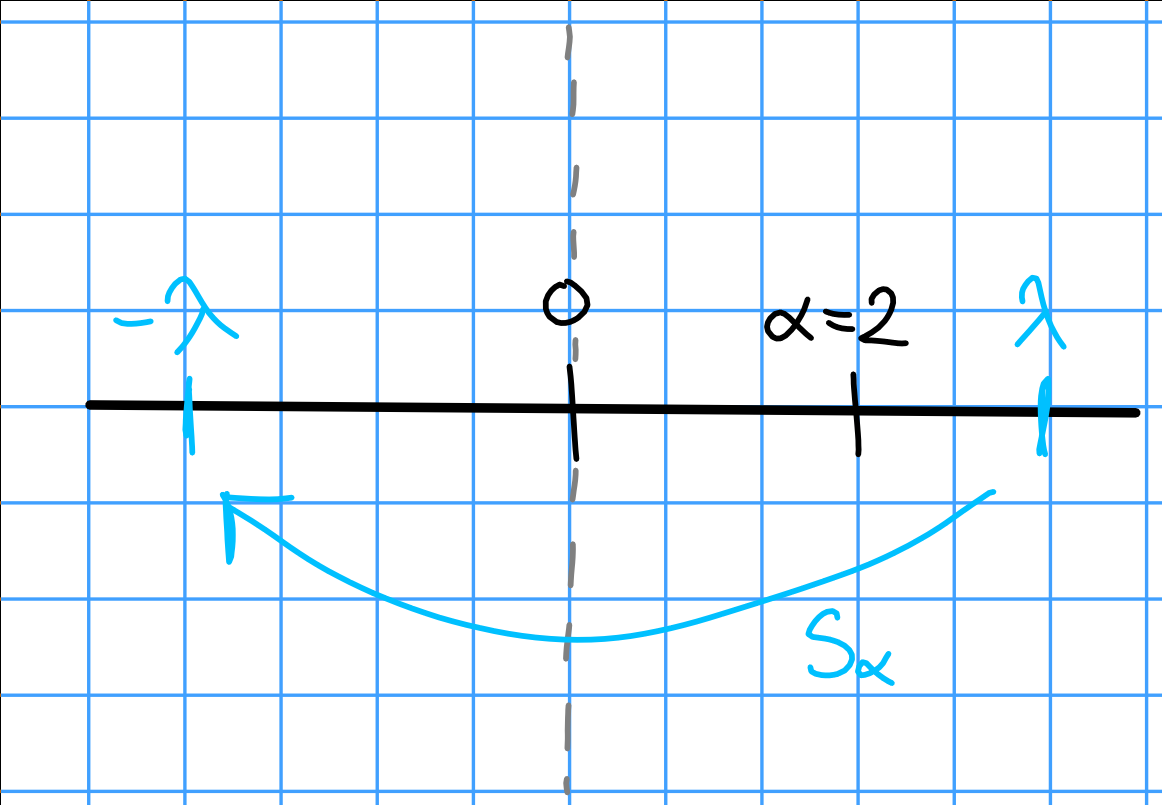
\includegraphics[width=2.60417in,height=\textheight]{figures/2020-01-15-09:38.png}
\caption{Weyl group reflection in \(\liesl_2(\CC)\)}
\end{figure}

\hypertarget{chapter-1-category-mathcal-o-basics}{%
\section{\texorpdfstring{Chapter 1: Category \(\mathcal O\)
Basics}{Chapter 1: Category \textbackslash mathcal O Basics}}\label{chapter-1-category-mathcal-o-basics}}

The category of \(U(\lieg)\dash\)modules is too big. Motivated by work
of Verma in 60s, started by Bernstein-Gelfand-Gelfand in the 1970s. Used
to solve the Kazhdan-Lusztig conjecture.

\hypertarget{axioms-and-consequences}{%
\subsection{Axioms and Consequences}\label{axioms-and-consequences}}

\begin{definition}[Category $\OO$]

\(\mathcal O\) is the full subcategory of \(U(\lieg)\) modules
consisting of \(M\) such that

\begin{enumerate}
\def\labelenumi{\arabic{enumi}.}
\tightlist
\item
  \(M\) is finitely generated as a \(U(\lieg)\dash\)module.
\item
  \(M\) is \(\lieh\dash\)semisimple, i.e.~\(M\) is a weight module
  \begin{align*}
  M = \bigoplus_{\lambda \in \lieh\dual} M_\lambda
  \end{align*}
\item
  \(M\) is locally \(n\dash\)finite, i.e.~
  \begin{align*}  
  \dim_\CC U(\lien) v < \infty \qquad \forall v\in M
  .\end{align*}
\end{enumerate}

\end{definition}

\begin{example}[?]

If \(\dim M < \infty\), then \(M\) is \(\lieh\dash\)semisimple, and
axioms 1, 3 are obvious.

\end{example}

\begin{lemma}[?]

Let \(M \in \OO\), then

\begin{enumerate}
\def\labelenumi{\arabic{enumi}.}
\setcounter{enumi}{3}
\tightlist
\item
  \(\dim M_\mu < \infty\) for all \(\mu \in \lieh\dual\).
\item
  There exist \(\lambda_1, \cdots \lambda_r \in \lieh\dual\) such that
  \begin{align*}
  \Pi(M) \subset \Union_{i=1}^\lambda (\lambda_i - \ZZ^+ \Phi^+)
  \end{align*}
\end{enumerate}

\begin{figure}
\centering
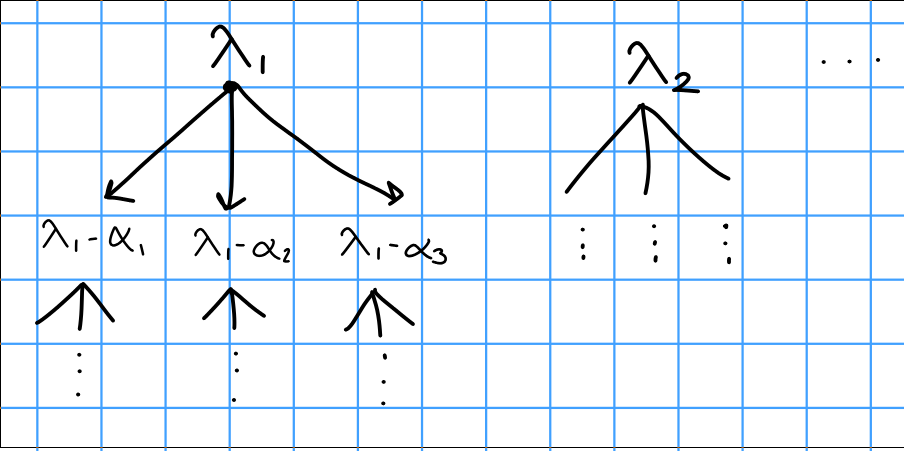
\includegraphics[width=3.64583in,height=\textheight]{figures/2020-01-15-09:50.png}
\caption{Forest structure of weights}
\end{figure}

\end{lemma}

\begin{proof}[?]

By axiom 2, every \(v\in M\) is a finite sum of weight vectors in \(M\).
We can thus assume that our finite generating set consists of weight
vectors. We can then reduce to the case where \(M\) is generated by a
single weight vector \(v\). So consider \(U(\lieg) v\). By the PBW
theorem, there is a triangular decomposition
\begin{align*}
U(\lieg) = U(\lien^-) U(\lieh) U(\lien)
\end{align*}

By axiom 3, \(U(\lien) \cdot v\) is finite dimensional, so there are
finitely many weights of finite multiplicity in the image. Then
\(U(\lieh)\) acts by scalar multiplication, and \(U(\lien^-)\) produces
the ``cones'' that result in the tree structure:

\begin{figure}
\centering
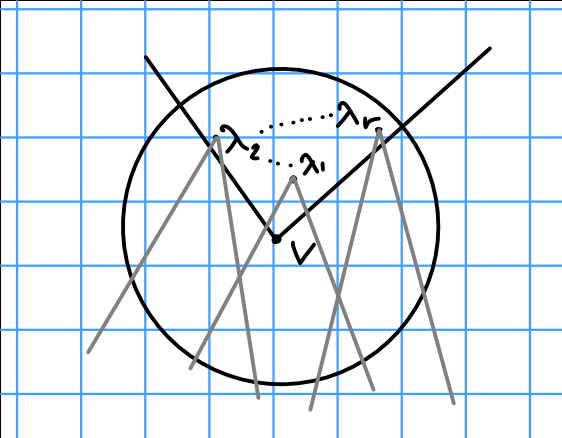
\includegraphics[width=3.64583in,height=\textheight]{figures/2020-01-15-09:57.png}
\caption{Cones under tree structure of weights}
\end{figure}

A weight of the form \(\mu = \lambda_i - \sum n_i \alpha_i\) can arise
from \(y_{n_1}^{n_1} \cdots\).

\todo[inline]{Missing end of lecture.}

\end{proof}

\hypertarget{friday-january-17th}{%
\section{Friday January 17th}\label{friday-january-17th}}

Let \(M\)

\begin{enumerate}
\def\labelenumi{\arabic{enumi}.}
\tightlist
\item
  Be finitely generated,
\item
  Semisimple \(M = \oplus_{\lambda \in \lieh\dual} M_\lambda\),
\item
  Locally finite
\item
  \(\dim M_\mu < \infty\) for all \(\mu \in \lieh\dual\),
\item
  Satisfy the forest condition for weights.
\end{enumerate}

\begin{theorem}[Properties of $\OO$]

\envlist

\begin{enumerate}
\def\labelenumi{\alph{enumi}.}
\item
  \(\mathcal O\) is Noetherian \footnote{Ascending chain condition on
    submodules, i.e.~no infinite filtrations by submodules.}
\item
  \(\mathcal O\) is closed under quotients, submodules, finite direct
  sums
\item
  \(\mathcal O\) is abelian (similar to a category of modules)
\item
  If \(M\in \mathcal O\), \(\dim L < \infty\), then
  \(L \tensor M \in \mathcal O\) and the endofunctor
  \(M \mapsto L\tensor M\) is exact
\item
  If \(M\in \mathcal O\), then \(M\) is locally \(Z(\lieg)\dash\)finite
  \footnote{Recall: this is the center of \(U(\lieg)\)),
    i.e.~\(\dim\spanof ~Z(\lieg)v < \infty\) for all \(v\in M\).}
\item
  \(M\in \mathcal O\) is a finitely generated \(U(\lien^-)\dash\)module.
\end{enumerate}

\end{theorem}

\begin{proof}[of a and b]

See BA II, page 103.

\end{proof}

\begin{proof}[of c]

Implied by (b), BA II Page 330.

\end{proof}

\begin{proof}[of d]

Can check that \(L\tensor M\) satisfies 2 and 3 above. Need to check
first condition. Take a basis \(\theset{v_i}\) for \(L\) and
\(\theset{w_j}\) a finite set of generators for \(M\). The claim is that
\(B = \theset{v_i \tensor w_j}\) generates \(L\tensor M\). Let \(N\) be
the submodule generated by \(B\).

For any \(v\in V\), \(v\tensor w_j \in N\). For arbitrary
\(x\in \lieg\), compute
\begin{align*}x\cdot(v\tensor w_j) = (x\cdot v) \tensor w_j + x\tensor (v\cdot w_j).\end{align*}
Since the LHS is in \(N\) and the first term on the RHS is in \(N\), the
entire RHS is in \(N\). By iterating, we find that
\(v\tensor (u\cdot w_j) \in N\) for all PBW monomials \(u\). So
\(L\tensor M \in \mathcal O\).

\end{proof}

\begin{proof}[of e]

Since \(v\in M\)is a sum of weight vectors, wlog we can assume
\(v \in M_\lambda\) is a weight vector (where
\(\lambda \in \lieh\dual\)). For any central element \(z\in Z(\lieg)\),
we can compute
\begin{align*}h\cdot(z\cdot v) = z \cdot (h\cdot v) = z \cdot \lambda(h) v = \lambda(h)z \cdot v.\end{align*}
Thus \(z\cdot v\in M_\lambda\). By (4), we know that
\(\dim M_\lambda < \infty\), so \(\dim \spanof ~Z(\lieg) v < \infty\) as
well.

\end{proof}

\begin{proof}[of f]

By 5, \(M\) is generated by a finite dimensional \(U(\mathfrak b)\)
submodule \(N\). Since we have a triangular decomposition
\(U(\lieg) = U(\lien^-) U(\mathfrak b)\), there is a basis of weight
vectors for \(N\) that generates \(M\) as a \(U(\lien^-)\) module.

\end{proof}

\hypertarget{highest-weight-modules}{%
\subsection{Highest Weight Modules}\label{highest-weight-modules}}

\begin{definition}[Maximal Vector]

A \textbf{maximal vector} \(v^+ \in M \in \mathcal O\) is a nonzero
vector such that \(\lien \cdot v^+ = 0\).

\end{definition}

\begin{remark}

By properties 2 and 3, every nonzero \(M\in \mathcal O\) has a maximal
vector.

\end{remark}

\begin{definition}[Highest Weight Modules]

A \textbf{highest weight module} \(M\) of highest weight \(\lambda\) is
a module generated by a maximal vector of weight \(\lambda\), i.e.~
\begin{align*}M = U(\lieg) v^+ = U(\lien^-) U(\lieh) U(\lien) v^+ = U(\lien^-) v^+\end{align*}

\end{definition}

\begin{theorem}[Properties of Highest Weight Modules]

Let \(M = U(\lien^-)v^+\) be a highest weight module, where
\(v^+ \in M_\lambda\). Fix
\(\Phi^+ = \theset{\beta_1, \cdots, \beta_n}\) with root vectors
\(y_i \in \lieg_{\beta_i}\).

\begin{enumerate}
\def\labelenumi{\alph{enumi}.}
\item
  \(M\) is the \(\CC\dash\)span of PBW monomials
  \(\generators{ y_1^{t_1} \cdots y_m^{t_m}}\) of weight
  \(\lambda - \sum t_i \beta_i\). Thus \(M\) is a module.
\item
  All weights \(\mu\) of \(M\) satisfy \(\mu \leq \lambda\)
\item
  \(\dim M_\mu < \infty\) for all \(\mu \in T(M)\), and
  \(\dim M_\lambda = 1\). In particular, property (3) holds and
  \(M \in \mathcal O\).
\item
  Every nonzero quotient of \(M\) is a highest-weight module of highest
  weight \(\lambda\).
\item
  Every submodule of \(M\) is a weight module, and any submodule
  generated by a maximal vector with \(\mu < \lambda\) is proper. If
  \(M\) is semisimple, then the set of maximal weight vectors equals
  \(\CC\units v^+\).
\item
  \(M\) has a unique maximal submodule \(N\) and a unique simple
  quotient \(L\), thus \(M\) is indecomposable.
\item
  All simple highest weight modules of highest weight \(\lambda\) are
  isomorphic.
\end{enumerate}

\end{theorem}

\begin{remark}

For such \(M\), \(\dim \endo(M) = 1\). (Category \(\mathcal O\) version
of Schur's Lemma, generalizes to infinite dimensional case)

\end{remark}

\begin{proof}[a through e]

Either obvious or follows from previous results. First few imply \(M\)
is in \(\mathcal O\), and we know the latter hold for such modules.

\end{proof}

\begin{proof}[of f]

\(N\) is a sum of submodules, so \(N = \sum M_i\), proper submodules of
\(M\). So take \(L = M/N\). To see indecomposability, there exists a
better proof in section 1.3.

\end{proof}

\begin{proof}[of g]

Let \(M_1 = U(\lien^-)v_1^+\) and \(M_2\) be define similarly, where the
\(v_i \in (M_i)_\lambda\) have the same weight. Then
\(M_0 \definedas M_1 \oplus M_2\) implies that
\(v^+ \definedas (v_1^+, v_2^+)\) is a maximal vector for \(M_0\). So
\(N \definedas U(\lien^-) v^+\) is a highest weight module of highest
weight \(\lambda\).

We have the following diagram:

\begin{center}\includesvg[width=0.7\linewidth]{36708efc5354c8b43f189c51a81ea09cb9578285}\end{center}

and since e.g.~\(N \to M_1\) is not the zero map, it is a surjection.

By (f), \(N\) is a unique simple quotient, so this forces
\(M_1 \cong M_2\). Since \(M\) is simple, any nonzero
\(\lieg\dash\)endomorphism \(\phi\) must be an isomorphism, and so we
take \(v^+ \mapsto cv^+\) for some \(c\neq 0\). Note that since \(\phi\)
is also a \(\lieh\dash\)morphism, we have \(\dim M_\lambda = 1\).

Since \(v^+\) generates \(M\) and
\begin{align*}
\phi(u\cdot v^+) = u \phi(v^+) = cu\cdot v^+
,\end{align*} \(\phi\) is multiplication by a constant.

\end{proof}

\hypertarget{wednesday-january-22nd}{%
\section{Wednesday January 22nd}\label{wednesday-january-22nd}}

\begin{exercise}[?]

Try problems 1.1 and 1.3* in Humphreys.

\end{exercise}

\textbf{Recall:} In category \(\mathcal O\), we have finite dimensional,
semisimple modules over \(\CC\) with triangular decompositions.

If \(M\) is any \(U(\lieg)\) module than a \(v^+ \in M_\lambda\) a
weight vector (so \(\lambda \in \lieh\dual\)) is primitive iff
\(\lien \cdot v^+ = 0\). Note: it doesn't have to be of maximal weight.
\(M\) is a highest weight module of highest weight \(\lambda\) iff it's
generated over \(U(\lieg)\) as an associative algebra by a maximal
vector \(v^+\) of weight \(\lambda\). Then \(M = U(\lieg) \cdot v^+\).

See structure of highest weight modules, and irreducibility.

\begin{corollary}[?]

If \(0 \neq M\in\mathcal O\), then \(M\) has a finite filtration with
quotients highest weight modules,
i.e.~\(M_0 \subset M_1 \subset \cdots \subset M_n = M\) with
\(M_i/M_{i-1}\) highest weight modules.

\end{corollary}

Note that the quotients are not necessarily simple, so this isn't a
composition series, although we'll show such a series exists later.

\begin{theorem}[Module Span of Weight Vectors is Finite Dimensional]

Let \(V\) be the \(\lien\) submodule of \(M\) generated by a finite set
of weight vectors which generate \(M\) as a \(U(\lieg)\) module,
i.e.~take the finite set of weight vectors and act on them by
\(U(\lien)\). Then \(\dim_\CC V < \infty\) since \(M\) is locally
\(\lien\dash\)finite.

\end{theorem}

Note that \(\lien\) increases weights.

\begin{proof}[?]

Induction on \(n = \dim V\). If \(n=1\), \(M\) itself is a highest
weight module. For \(n > 1\), choose a weight vector \(v_1 \in V\) of
weight \(\lambda\) which is maximal among all weights of \(V\). Set
\(M_1 \definedas U(\lieg) v_1\); this is a highest weight submodule of
\(M\) of highest weight \(\lambda\). (\(\lien\) has to kill v\_1,
otherwise it increases weight and \(v_1\) wouldn't be maximal.)

Let \(\bar M = M/M_1 \in \mathcal O\), this is generated by the image of
\(\bar V\) of \(V\) and thus \(\dim \bar V < \dim V\). By the IH,
\(\bar M\) has the desired filtration, say
\begin{align*}0 \subset \bar M_2 \subset \bar M_{n-1} \subset \bar M_n = \bar M.\end{align*}
Let \(\pi: M \to M/M_1\), then just take the preimages
\(\pi\inv(\bar M_i)\) to be the filtration on \(M\).

\end{proof}

\begin{remark}

By isomorphism theorems, the quotients in the series for \(M\) are
isomorphic to the quotients for \(\bar M\).

\end{remark}

\hypertarget{verma-and-simple-modules}{%
\subsection{Verma and Simple Modules}\label{verma-and-simple-modules}}

Constructing \emph{universal} highest weight modules using ``algebraic
induction''. Start with a nice subalgebra of \(\lieg\) then ``induce''
via \(\tensor\) to a module for \(\lieg\).

Recall \(\lieg = \lien^- \oplus \lieh \oplus \lien\), here
\(\lieh \oplus \lien\) is the Borel subalgebra \(\lieb\), and \(\lien\)
corresponds to a fixed choice of positive roots in \(\Phi^+\) with basis
\(\Delta\). Then \(U(\lieg) = U(\lien^-) \tensor_\CC U(\lieb)\). Given
any \(\lambda \in \lieh\dual\), let \(\CC_\lambda\) be the 1-dimensional
\(\lieh\dash\)module (i.e.~1-dimensional \(\CC\dash\)vector space)on
which \(\lieh\) acts by \(\lambda\).

Let \(\theset{1}\) be the basis for \(\CC\), so
\(h \cdot 1 = \lambda(h)1\) for all \(h\in \lieh\). Then there is a map
\(\lieb \to \lieb / \lien \cong \lieh\), so make \(C_\lambda\) a
\(\lieb\dash\)module via this map. This ``inflate'' \(C_\lambda\) into a
1-dimensional \(\lieb\dash\)module.

Note that \(\lieh\) is solvable, and by Lie's Theorem, every finite
dimensional irreducible \(\lieb\dash\)module is of the form
\(\CC_\lambda\) for some \(\lambda \in \lieh\dual\).

\begin{definition}[Verma Modules]

\begin{align*}
M(\lambda) \da U(\lieg) \tensor_{U(\lieb)} \CC_\lambda \definedas \ind_\lieb^\lieg \CC_\lambda
\end{align*} is the \emph{Verma module of highest weight \(\lambda\)}.

\end{definition}

This process is called \textbf{algebraic/tensor induction}. This is a
\(U(\lieg)\) module via left multiplication, i.e.~acting on the first
tensor factor.

\begin{remark}

Since \(U(\lieg) \cong U(\lien^-) \tensor_\CC U(\lieh)\), we have
\(M(\lambda) \cong U(\lien^-) \tensor_\CC \CC_\lambda\), but at what
level of structure?

\begin{itemize}
\tightlist
\item
  As a vector space (clear)
\item
  As a \(\lien^-\dash\)module via left multiplication
\item
  As a \(\lieh^-\dash\)module via the \(\tensor\) action.
\end{itemize}

In particular, \(M(\lambda)\) is a \emph{free} \(U(\lien^-)\dash\)module
of rank 1. Note that this always happens when tensoring with a vector
space.

\end{remark}

Consider \(v^+ \definedas 1\tensor 1 \in M(\lambda)\). Note that
\(U(\lien^-)\) is not homogeneous, so not graded, but does have a
filtration. Then \(v^+\) is nonzero, and freely generates \(M(\lambda)\)
as a \(U(\lien^-)\dash\)module. Moreover \(\lien \cdot v^+ = 0\) since
for \(x\in \lieg_\beta\) for \(\beta \in \Phi^+\), we have

\begin{align*}
x(1\tensor 1) &= x\tensor 1  \\
&= 1\tensor x\cdot 1 \quad\text{since } x\in \lieb \\
&= 1 \tensor 0 \implies x\in \lien \\
&= 0
,\end{align*}

and for \(h\in \lieh\),

\begin{align*}
h(1\tensor 1) 
&= h1\tensor 1 \\
&= 1 \tensor h1\\
&=1 \tensor \lambda(h) 1 \\
&=\lambda(h) v^+
.\end{align*}

So \(M(\lambda)\) is a highest weight module of highest weight
\(\lambda\), and thus \(M(\lambda) \in \mathcal O\).

\begin{remark}

Any weight \(\lambda \in \lieh\dual\) is the highest weight of some
\(M\in \mathcal O\). Let \(\Pi(M)\) denote the set of weights of a
module, then \(\Pi(M(\lambda)) = \lambda - \ZZ^+ \Phi^+\).

By PBW, we can obtain a basis for \(M(\lambda)\) as
\(\theset{ y_1^{t_1} \cdots y_m^{t_m}v^+ \suchthat t_i \in \ZZ^+}\).
Taking a fixed ordering \(\theset{\beta_1, \cdots, \beta_m} = \Phi^+\),
then \(0\neq y_i \in \lieg_{-\beta_i}\). Then every weight of this form
is a weight of some \(M(\lambda)\), and every weight of \(M(\lambda)\)
is of this form: \(\lambda - \sum t_i \beta_i\).

\end{remark}

\begin{remark}

The functor \(\Ind_\lieh^\lieg(\wait) = U(\lieg) \tensor_{\lieb} \wait\)
from the category of finite-dimensional \(\lieg\dash\)semisimple
\(\lieb\dash\)modules to \(\mathcal O\) is an exact functor, since it is
naturally isomorphic to \(U(\lien^-) \tensor_\CC \wait\) (which is
clearly exact since we are tensoring a vector space over its ground
field).

\end{remark}

\begin{proposition}[Alternate construction of $M(\lambda)$]

Let \(I\) by a left ideal of \(U(\lieg)\) which annihilates \(v^+\), so
\begin{align*}
I = \generators{\lien, h-\lambda(h)\cdot 1 \suchthat h\in\lieh}
.\end{align*} Since \(v^+\) generates \(M(\lambda)\) as a
\(U(\lieg)\dash\)module, then (by a standard ring theory result)
\(M(\lambda) = U(\lieg)/I\), since \(I\) is the annihilator of
\(M(\lambda)\).

\end{proposition}

\begin{theorem}[Universal Property of Verma Modules]

Let \(M\) be any highest weight module of highest weight \(\lambda\)
generated by \(v\). Then \(I\cdot v = 0\), so \(I\) is the annihilator
of \(v\) and thus \(M\) is a quotient of \(M(\lambda)\). Thus
\(M(\lambda)\) is universal in the sense that every other highest weight
module arises as a quotient of \(M(\lambda)\).

\end{theorem}

\begin{remark}

By theorem 1.2, \(M(\lambda)\) has a unique maximal submodule
\(N(\lambda)\) (nonstandard notation) and a unique simple quotient
\(L(\lambda)\) (standard notation).

\end{remark}

\begin{theorem}[Characterization of Simple Modules and Schur's Lemma]

Every simple module in \(\mathcal O\) is isomorphic to \(L(\lambda)\)
for some \(\lambda \in \lieh\dual\) and is determined uniquely up to
isomorphism by its highest weight. Moreover, there is an analog of
Schur's lemma:
\begin{align*}\dim \hom_{\mathcal O}(L(\mu), L(\lambda)) = \delta_{\mu\lambda}\end{align*},
i.e.~it's 1 iff \(\lambda=\mu\) and 0 otherwise.

\end{theorem}

\begin{remark}

Up to isomorphism, we've found all of the simple modules in
\(\mathcal O\), and most are finite-dimensional.

\end{remark}

\hypertarget{friday-january-24th}{%
\section{Friday January 24th}\label{friday-january-24th}}

A standard theorem about classifying simple modules in category \(\OO\):

\begin{description}
\item[Theorem (Classification of Simple Modules)]
Every simple module in \(\OO\) is isomorphic to \(L(\lambda)\) for some
\(\lambda \in \lieh\dual\), and is determined uniquely up to isomorphism
by its highest weight. Moreover,
\(\dim \hom_\OO(L(\mu), L(\lambda)) = \delta_{\lambda \mu}\).
\item[Proof]
Let \(L \in \OO\) be irreducible. As observed in 1.2, \(L\) has a
maximal vector \(v^+\) of some weight \(\lambda\).

Recall: can increase weights and reach a maximal in a finite number of
steps.

Since \(L\) is irreducible, \(L\) is generated by that weight vector,
i.e.~\(L U(\lieg) \cdot v^+\), so \(L\) must be a highest weight module.

\begin{quote}
Standard argument: use triangular decomposition.
\end{quote}

By the universal property, \(L\) is a quotient of \(M(\lambda)\). But
this means \(L \cong L(\lambda)\), the unique irreducible quotient of
\(M(\lambda)\).

By Theorem 1.2 part g (see last Friday),
\(\dim \endo_\OO(L(\lambda)) = 1\) and
\(\hom_\OO(L(\mu), L(\lambda)) = 0\) since both entries are irreducible.
\item[Theorem (1.2 f, Highest Weight Modules are Indecomposable)]
A highest weight module \(M\) is indecomposable, i.e.~can't be written
as a direct sum of two nontrivial proper submodules.
\item[Proof (of Theorem 1.2 f)]
Suppose \(M = M_1 \oplus M_2\) where \(M\) is a highest weight module of
highest weight \(\lambda\). Category \(\OO\) is closed under submodules,
so \(M_i\) are weight modules and have weight-space decompositions. But
\(M_\lambda\) is 1-dimensional (triangular decomposition, only \(\CC\)
acts), and thus \(M_\lambda \subset M_1\). Since \(M_\lambda\) is a
highest weight module, it generates the entire module, so
\(M \subset M_1\). The reverse holds as well, so \(M = M_1\) and this
forces \(M_2 = 0\).
\end{description}

\hypertarget{maximal-vectors-in-verma-modules}{%
\subsection{1.4: Maximal Vectors in Verma
Modules}\label{maximal-vectors-in-verma-modules}}

\begin{quote}
1.5: Examples in the case \(\liesl(2)\), over \(\CC\) as usual.
\end{quote}

First, some review from Lie algebras.

Let \(\lieg\) be any lie algebra, and take \(u, v \in U(\lieg)\). Recall
that we have the formula
\begin{align*}uv = [uv] + vu,\end{align*} where we use the definition
\([uv] = uv - vu\).

Let \(x, y_1, y_2\) be in \(\lieg\), what is \([x, y_1 y_2]\)? Use the
fact that \(\ad x (y_1, y_2)\) acts as a derivation, and so
\([x, y_1 y_2] = [x y_1]y_2 + y_1[x y_2]\), which is a bracket entirely
in the Lie algebra. This extends to an action on \(U(\lieg)\) by the
product rule.

Recall that \(\liesl(2)\) is spanned by
\(y =[0,0; 1,0], h = [1,0; 0, -1], x = [0,1; 0,0]\), where each basis
vector spans \(\lien^-, \lieh, \lien\) respectively. Then
\([x y] = h, [h x] = 2x, [h y] = -2y\), so
\(E_{ij} E_{kl} = \delta_{jk} E_{il}\) (should be able to compute
easily!).

Then \(\lieh = \CC\), so \(\lieh\dual \cong \CC\) where
\(\lambda \mapsto \lambda(h)\). So we identify \(\lambda\) with a
complex number, this is kind of like a bundle of Verma modules over
\(\CC\).

Consider \(M(1)\), then \(\lambda = 1\) will denote \(\lambda(h) = 1\).
As in any Verma module,
\(M(\lambda) \cong U(\lien^-) \tensor_\CC \CC_{\lambda}\). We can think
of \(v^+\) as \(1\tensor 1\), with the action \(yv^+ = y1\tensor 1\).
Note that \(y\) has weight \(-2\).

\begin{longtable}[]{@{}ll@{}}
\toprule
Weight & Basis\tabularnewline
\midrule
\endhead
1 & \(v^+\)\tabularnewline
-1 & \(yv^+\)\tabularnewline
-3 & \(y^2 v^+\)\tabularnewline
-5 & \(y^3 v^+\)\tabularnewline
\bottomrule
\end{longtable}

Consider how \(x\actson y^2 v^+\). Note that \(x\) has weight \(+2\). We
have

\begin{align*}
x \cdot y^2 v^+ 
&= x \cdot y^2 \tensor 1_\lambda \\
&= ([x y^2] + y^2 x) \tensor 1 \\
&= ([xy]y + y[xy]) \tensor 1 + y^2 \tensor x\cdot 1 \quad\text{moving $x$ across the tensor because ?}\\
&= ([xy]y + y[xy]) \tensor 1 + 0  \quad\text{since $x$ is maximal} \\
&= (hy + yh) \tensor 1 \\
&= hy \tensor 1 + y\tensor h\cdot 1 \\
&= hy \tensor 1 + \lambda(h)1 \\
&= hy \tensor 1 + 1 \\
&= ([xy] + yh)\tensor 1 + y\tensor 1 \\
&= -2y \tensor 1 + y\tensor 1 + y\tensor 1 \\
&= 0
.\end{align*}

So \(y\) moves us downward through the table, and \(x\) moves upward,
except when going from \(-3\to -1\) in which case the result is zero.

Thus there exists a morphism \(\phi: M(-3) \to M(1)\), with image
\(U(\lieg) y^2 v^+ = U(\lien^-) y^2 v^+\). So the image of \(\phi\) is
everything spanned by the bases in the rows \(-3, -5, \cdots\), which is
exactly \(M(-3)\). So \(M(-3) \injects M(1)\) as a submodule.

\begin{quote}
Motivation for next section: we want to find Verma modules which are
themselves submodules of Verma modules.
\end{quote}

It turns out that \(\im \phi \cong N(1)\). We should have
\(M(1) / N(1) \cong L(1)\). What is the simple module of weight 1 for
\(\liesl(2)\)? The weights of \(L(n)\) are \(n, n-2, n-4, \cdots, -n\),
so the representations are parameterized by \(n\in \ZZ^{+}\). These are
the Verma modules for \(\liesl(2)\). What happens is that
\(y\actson -n \to -n-2\) gives a maximal vector, so the calculation
above roughly goes through the same way. So we'll have a similar picture
with \(L(n)\) at the top.

\hypertarget{back-to-1.4}{%
\subsection{Back to 1.4}\label{back-to-1.4}}

\emph{Question 1:} What are the submodules of \(M(\lambda)\)?

\emph{Question 2:} What are the Verma submodules
\(M(\mu) \subset M(\lambda)\)? Equivalently, when do maximal vectors of
weight \(\mu < \lambda\) (the interesting case) lie in \(M(\lambda)\)?

\emph{Question 3:} As a special case, when do maximal vectors of weight
\(\lambda - k\alpha\) for \(\alpha \in \Delta\) lie in \(M(\lambda)\)
for \(k\in \ZZ^+\)?

Fix a Chevalley basis for \(\lieg\) (see section 0.1)
\(h_1, \cdots, h_\ell \in \lieh\) and \(x_\alpha \in \lieg_\alpha\) and
\(y_\alpha \in \lieg_{-\alpha}\) for \(\alpha \in \Phi^+\). Let
\(\Delta = \theset{\alpha_1, \cdots, \alpha_\ell}\) and let
\(x_i = x_{\alpha_i}, y_i = y_{\alpha_i}\) be chosen such that
\([x_i y_i] = h_i\).

\begin{description}
\item[Lemma]
For \(k\geq 0\) and \(1\leq i, j \leq \ell\), then

\begin{enumerate}
\def\labelenumi{\alph{enumi}.}
\item
  \([x_j, y_i^{k+1}] = 0\) if \(j\neq i\)
\item
  \([h_j, y_i^{k+1}] = -(k+1) \alpha_i(h_j) y_i^{k+1}\).
\item
  \([x_i, y_i^{k+1}] = -(k+1) y_i(k\cdot 1 - h_i)\).
\end{enumerate}
\item[Proof (sketch)]
Both easy to prove by induction since
\([x_j, y_i] \to \alpha_j - \alpha_i \not\in \Phi\) is a difference of
simple roots.

For \(k=0\), all identities are easy. For \(k> 0\), an inductive formula
that uses the derivation property, which we'll do next class.
\end{description}

\hypertarget{monday-january-27th}{%
\section{Monday January 27th}\label{monday-january-27th}}

\hypertarget{section-1.4}{%
\subsection{Section 1.4}\label{section-1.4}}

Fix \(\Delta = \theset{\alpha_1, \cdots, \alpha_\ell}\),
\(x_i \in g_{\alpha_i}\) and \(y_i \in g_{-\alpha_i}\) with
\(h_i = [x_i y_i]\).

\begin{description}
\item[Lemma]
For \(k\geq 0\) and \(1 \leq i, j \leq \ell\),

\begin{enumerate}
\def\labelenumi{\alph{enumi}.}
\tightlist
\item
  \([x_j y_i^{k+1}] = 0\) if \(j\neq i\)
\item
  \([h_j y_i^{k+1}] = -(k+1) \alpha_i(h_j) y_i^{k+1}\)
\item
  \([x_i y_i^{k+1}] = (k+1) y_i^{k} (k\cdot 1 - h_i)\).
\end{enumerate}
\item[Proof (Sketch for (c))]
By induction, where \(k=0\) is clear.

\begin{align*}
[x+i y_i^{k+1}]
&= [x_i y_i] y_i^k + y_i [x_i y_i^k] \\
&=h_i y_i^k + y_i(-k y_i^{k-1} ((k-1)1 - h_i)) \quad\text{by I.H.} \\
&= (k+1)y_i^k h_i - (k^2 -k + 2k)y_i^k \\
&= -(k+1) y_i^k ( k\cdot 1 - h_i )
.\end{align*}
\item[Proposition (Existence of Morphisms of Verma Modules)]
Suppose \(\lambda \in \lieh\dual, \alpha \in \Delta\), and
\(n\definedas (\lambda, \alpha\dual) \in \ZZ^+\). Then in
\(M(\lambda)\), \(y_\alpha^{n+1} v^+\) is a maximal weight vector of
weight \(\mu \definedas \lambda - (n+1)\alpha < \lambda\).

\begin{quote}
Note this is free as an \(U(\lien^-)\dash\)module, so \(v^+ \neq 0\).
Note that \(n = \lambda(h_\alpha)\).
\end{quote}

By the universal property, there is a nonzero homomorphism
\(M(\mu) \to M(\lambda)\) with image contained in \(N(\lambda)\), the
unique maximal proper submodules of \(M(\lambda)\).
\item[Proof]
Say \(\alpha = \alpha_i\). Fix \(j\neq i\).

\begin{align*}
x_i y_\alpha^{n+1} \tensor 1 
&= [x_j y_i^{n+1}] \tensor 1 + y_i^{n+1} \tensor x_j \cdot 1 \\
&= [x_j y_i^{n+1}] \tensor 1 + y_i^{n+1} \tensor 0 \quad\text{by a} \\
&= 0
.\end{align*}

\begin{align*}
x_i y_i^{n+1} \tensor 1 
&= [x_i y_i^{n+1} \tensor 1] \\
&= -(n+1) y_i^n (n\cdot 1 - h_i) \tensor 1 \\
&= -(n+1) (n - \lambda(h_i)) 1 \tensor 1 \\
&\definedas -(n+1) (\lambda(h_i) - \lambda(h_i)) 1 \tensor 1 \\
&= 0
.\end{align*}

Since \(g_{\alpha_j}\) generate \(\lien\) as a Lie algebra, since
\([\lieg_\alpha, \lieg_\beta] = \lieg_{\alpha + \beta}\). This shows
that \(\lien \cdot y_i^{n+1} v^+ = 0\), and the weight of
\(y_i^{n+1} v^+\) is \(\lambda - (n+1)\alpha_i\). So \(y_i^{n+1}\) is a
maximal vector of weight \(\mu\). The universal property implies there
is a nonzero map \(M(\mu) \to M(\lambda)\) sending highest weight
vectors to highest weight vectors and preserving weights. The image is
proper since all weights of \(M_\mu\) are less than or equal to
\(\mu < \lambda\).
\end{description}

Consider \(\liesl(2)\), then \(M(1) \supset M(-3)\). Note that
reflecting through 0 doesn't send 1 to -3, but shifting the origin to
\(-1\) and reflecting about that with \(s_\alpha \cdot\) fixes this
problem. Note that \(L(1)\) is the quotient.

For \(\lambda \in \lieh\dual\) and \(\alpha \in \Delta\), we can compute
\(s_\alpha \cdot \lambda \definedas s_\alpha(\lambda + \rho) - \rho\)
where \(\rho = \sum_{j=1}^\ell e_i\). Then
\((w_j, \alpha_i\dual) = \delta_{ij}\) and
\((\rho, \alpha_i\dual) = 1\).

\begin{align*}
s\alpha \cdot \lambda 
&= s_\alpha(\lambda + \rho) - \rho \\
&= (\lambda + \rho) - (\lambda + \rho, \alpha\dual)\alpha -\rho \\
&= \lambda + \rho - ((\lambda< \alpha\dual) +1)\alpha - \rho \\
&= \lambda - (n+1)\alpha \\
&= \mu
.\end{align*}

So this gives a well-defined, nonzero map
\(M(s_\alpha \cdot \lambda) \to M(\lambda)\) for
\(s_\alpha \cdot \lambda < \lambda\).

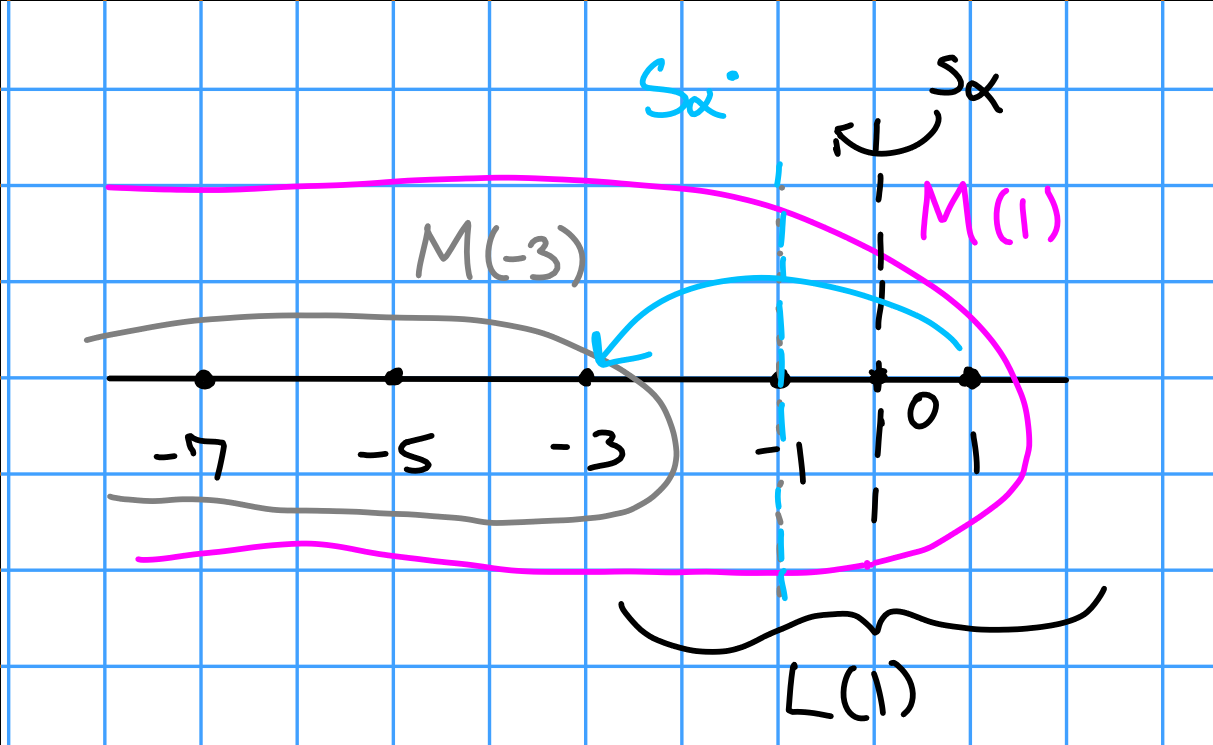
\includegraphics{figures/2020-01-27-09:35.png}\\

\begin{description}
\tightlist
\item[Corollary]
Let \(\lambda, \alpha, n\) be as in the above proposition. Let
\(\bar v^+\) now be a maximal vector of weight \(\lambda\) in
\(L(\lambda)\). Then \(y_\alpha^{n+1} \bar v^+ = 0\).
\item[Proof]
If not, then this would be a maximal vector, since it's the image of the
vector \(y_i^{n+1}v^+ \in M(\lambda)\) under the map
\(M(\lambda) \to L(\lambda)\) of weight \(\mu < \lambda\). Then it would
generate a proper submodules of \(L(\lambda)\), but this is a
contradiction since \(L(\lambda)\) is irreducible.
\end{description}

\hypertarget{section-1.5}{%
\subsection{Section 1.5}\label{section-1.5}}

Example: \(\liesl(2)\). What do Verma modules \(M(\lambda)\) and their
simple quotients \(L(\lambda)\) look like?

Fix a Chevalley basis \(\theset{y,h,x}\) and let
\(\lambda \in \lieh\dual \cong \CC\).

\begin{description}
\item[Fact 1]
For \(v^+ = 1\tensor 1_\lambda\), we have
\begin{align*}M(\lambda) = U(\lien^-) v^+ = \CC \generators{y^i v^+ \suchthat i\in \ZZ^+}\end{align*}
is a basis for \(M(\lambda)\) with weights \(\lambda - 2i\) where
\(\alpha\) corresponds to 2. So the weights of \(M(\lambda)\) are
\(\lambda, \lambda-2, \lambda-4, \cdots\) each with multiplicity 1.

Letting \(v_i = \frac 1 {i!} y^i v^+\) for \(i\in \ZZ^+\); this is a
basis for \(M(\lambda)\). Using the lemma, we have

\begin{align*}
h\cdot v_i &= (\lambda - 2i) v_i \\
y \cdot v_i &= (i+1) v_{i+1} \\
x\cdot v_i &= (\lambda - i + 1)v_{i-1} 
.\end{align*}

Note that these are the same for \emph{finite-dimensional}
\(\liesl(2)\dash\)modules, see section 0.9.
\item[Fact (2)]
We know from the proposition that if \(\lambda \in \ZZ^+\),
i.e.~\((\lambda, \alpha\dual) \in \ZZ^+\), then \(M(\lambda)\) has a
maximal vector of weight
\begin{align*}\lambda - (n+1)\alpha = \lambda - (\lambda+1)2 = -\lambda-2 = s_\alpha \cdot \lambda.\end{align*}
\item[Exercise]
Check that this maximal vector generates the maximal proper submodule
\begin{align*}N(\lambda) = M(-\lambda - 2).\end{align*}

So the quotient
\(L(\lambda) = M(\lambda) / N(\lambda) = M(\lambda) / M(-\lambda - 2)\)
has weights \(\lambda, \lambda-2, \cdots, -\lambda+2, -\lambda\). So
when \(\lambda \in \ZZ^+\), \(L(\lambda)\) is the familiar simple
\(\liesl(2)\dash\)module of highest weight \(\lambda\).
\item[Fact (3)]
When \(\lambda \not\in\ZZ^+\),

\begin{itemize}
\tightlist
\item
  \(N(\lambda) = \theset{0}\),
\item
  \(M(\lambda) = L(\lambda)\),
\item
  \(M(\lambda)\) is irreducible
\item
  \(L(\lambda)\) is infinite dimensional.
\end{itemize}
\item[Proof]
Argue by contradiction. If not, \(M(\lambda) \supset M \neq 0\) is a
proper submodule. So \(M\in \OO\), and thus \(M\) has a maximal weight
vector \(w^+\), and by the restriction of weights for modules in
\(\OO\), we know \(w^+\) has height \(\lambda - 2m\) for some
\(m\in \ZZ^+\). Then \(w^+ = c v_i\) where \(0\neq c \in \CC\), and
taking \(v_{-1} \definedas 0\) and
\(x\cdot v_i = (\lambda - i + 1)v_{i-1}\) for \(i\geq 1\), so
\(\lambda = i-1 \implies \lambda \in \ZZ^+\).
\end{description}

\hypertarget{friday-january-31st}{%
\section{Friday January 31st}\label{friday-january-31st}}

\begin{description}
\item[Theorem (Duals of Simple Quotients of Vermas)]
A useful formula: \(L(\lambda)\dual \cong L(-w_0)\).
\item[Proof]
\(L(\lambda)\dual\) is a finite dimensional module, and
\((x\cdot f)(v) = -f(x\cdot v)\), so \(L(\lambda)\dual \cong L(\nu)\)
for some \(\nu \in \Lambda^+\). The weights of \(L(\lambda)\dual\) are
the negatives of the weight of \(L(\lambda)\). Thus the lowest weight of
\(L(\lambda)\) is \(w_0\lambda\), since \(w_o\) reverses the partial
order on \(\lieh\dual\), i.e \(w_0 \Phi^+ = \Phi^-\)

Then
\begin{align*}
\mu \in \Pi(L(\mu)) \implies w_0 \mu \in \Pi(L(\lambda)) \implies w_0\mu \leq \lambda
.\end{align*} This shows that the lowest weight of \(L(\lambda)\) is
\(w_0 \lambda\), thus the highest weight \(L(\lambda)\dual\) is
\(-w_0 \lambda\) by reversing this inequality.

The inner product is \(W\) invariant and is its own inverse, so we can
move it to the other side.
\end{description}

\hypertarget{action-of-zlieg}{%
\subsection{\texorpdfstring{1.7: Action of
\(Z(\lieg)\)}{1.7: Action of Z(\textbackslash lieg)}}\label{action-of-zlieg}}

Next big goal: Every module in \(\OO\) has a \emph{finite} composition
series (Jordan-Holder series, the quotients are simple). Leads to
Kazhdan-Lustzig conjectures from 1979/1980, which were solved, but are
still open in characteristic \(p\) case.

The technique we'll use the Harish-Chandra homomorphism, which
identifies \(\mcz(\lieg)\) explicitly.

It's commutative, a subalgebra of a Noetherian algebra, no zero divisors
-- could be a quotient, but then it'd have zero divisors, so this seems
to force it to be a polynomial algebra on some unknown.

\begin{quote}
Also note that \(\mcz(\lieg) \definedas Z(U(\lieg))\).
\end{quote}

Recall: \(\mcz(\lieg)\) acts locally finitely on any \(M\in \OO\) --
this is by theorem 1.1e, i.e.~\(v\in M_\mu\) and \(z\in \mcz(\lieg)\)
implies that \(zv\in M_\mu\). (The calculation just follows by computing
the weight and commuting things through.)

Let \(\lambda \in \lieh\dual\) and \(M = U(\lieg)v^+\) a highest weight
module of highest weight \(\lambda\). Then for \(z\in \mcz(\lieg)\),
\(z\cdot v^+ \in M_\lambda\) which is 1-dimensional. Thus \(z\) acts by
scalar multiplication here, and \(z\cdot v^+ = \chi_\lambda(z) v^+\).
Now if \(u\in U(\lieu^-)\), we have
\begin{align*}z\cdot(u\cdot v^+) = u\cdot(z\cdot v^+) = u(\chi_\lambda(z)v^+) = \chi_\lambda(z) u\cdot v^+.\end{align*}
Thus \(z\) acts on \emph{all} of \(M\) by the scalar
\(\chi_\lambda(z)\).

\begin{description}
\tightlist
\item[Exercise]
Show that \(\chi_\lambda\) is a nonzero additive and multiplicative
function, so \(\chi_\lambda: \mcz(\lieg) \to \CC\) is linear and thus a
morphism of algebras. Conclude that \(\ker \chi_\lambda\) is a maximal
ideal of \(\mcz(\lieg)\).
\end{description}

Note: this is called the \emph{infinitesimal character}.

Note that \(\chi_\lambda\) doesn't depend on which highest weight module
\(M_\lambda\) was chosen, since they're all quotients of \(M(\lambda)\).
In fact, every submodule and subquotient of \(M(\lambda)\) has the same
infinitesimal character.

\begin{description}
\item[Definition (Central/Infinitesimal Character)]
\(\chi_\lambda\) is called the \emph{central (or infinitesimal)
character}, and \(\hat\mcz(\lieg)\) denotes the set of all central
characters. More generally, any algebra morphism
\(\chi: \mcz(\lieg) \to \CC\) is referred to as a central character.
Central characters are in one-to-one correspondence with maximal ideals
of \(\mcz(\lieg)\), where

\begin{align*}
\chi & \iff \ker \chi \\
\CC[x_1, \cdots, x_n] &\iff \generators{x_1 - a_1, \cdots, x_n - a_n}
\end{align*}

where \([a_1, \cdots, a_n] \in \CC^n\).
\end{description}

Next goal: Describe \(\chi_\lambda(z)\) more explicitly.

Using PBW, we can write
\(z\in \mcz(\lieg) \subset U(\lieg) = U(\lien^-) U(\lieh) U(\lien)\).
Some observations:

\begin{enumerate}
\def\labelenumi{\arabic{enumi}.}
\tightlist
\item
  Any PBW monomial in \(z\) ending with a factor in \(\lien\) will kill
  \(v^+\), and hence can not contribute to \(\chi_\lambda(z)\).
\item
  Any PBW monomial in \(z\) beginning with a factor in \(\lien^-\) will
  send \(v^+\) to a lower weight space, so it also can't contribute.
\end{enumerate}

So we only need to see what happens in the \(\lieh\) part. A relevant
decomposition here is
\begin{align*}
U(\lieg) = U(\lieh) \oplus \qty{ \lien^- U(\lieg) + U(\lieg)\lien^+  }
.\end{align*}

\begin{description}
\tightlist
\item[Exercise]
Why is this sum direct?
\end{description}

Let \(\mathrm{pr}: U(\lieg) \to U(\lieh)\) be the projection onto the
first factor. Then \(\chi_\lambda(z) = \lambda(\mathrm{pr} z)\) for all
\(z\in \mcz(\lieg)\). Then if
\(\mathrm{pr}(z) = h_1^{m_1} \cdots h_\ell^{m_\ell}\), we can extend the
action on \(\lieh\) to all polynomials in elements of \(\lieh\) (which
is in fact evaluation on these monomials), and thus
\(\chi_\lambda(z) = \lambda(h_1)^{m_1} \cdots \lambda(h_\ell)^{m_\ell}\).

Note that for \(\lambda \in \lieh\dual\), we've extended this to the
``evaluation map'' \(\lambda: U(\lieg) \cong S(\lieh)\), the symmetric
algebra on \(\lieh\).

Why is this the correct identification? The RHS is
\(T(\lieh) / \generators{x\tensor y - y\tensor x - [xy]}\), but notice
that the bracket vanishes since \(\lieh\) is abelian, and this is the
exact definition of the symmetric algebra.

Thus \(\chi_\lambda = \lambda \circ \mathrm{pr}\).

Observation:

\begin{align*}
\lambda(\mathrm{pr}(z_1 z_2))
&= \chi_\lambda(z_1 z_1)\\
&= \chi_\lambda(z_1) \chi_\lambda(z_2) \\
&= \cdots \\
&= \lambda( \mathrm{pr}(z_1) \mathrm{pr}(z_2) )
.\end{align*}

\begin{description}
\tightlist
\item[Exercise]
Show \(\intersect_{\lambda \in \lieh\dual} \ker \lambda = \theset{0}\).
\item[Definition (Harish-Chandra Morphism)]
Let
\(\xi = \restrictionof{\mathrm{pr}}{\mcz(\lieg)}: \mcz(\lieg) \to U(\lieh)\).
\item[Definition (Twisted Harish-Chandra Morphism)]
\(\xi\) is an algebra morphism, and is referred to as the
\emph{Harish-Chandra homomorphism}.
\end{description}

See page 23 for interpretation of \(\xi\) without reference to
representations.

Questions:

\begin{enumerate}
\def\labelenumi{\arabic{enumi}.}
\tightlist
\item
  Is \(\xi\) injective?
\item
  What is \(\im \xi \subset U(\lieh)\)?
\end{enumerate}

When does \(\chi_\lambda = \chi_\mu\)? Proved last time: we introduced
the \(\cdot\) action and proved that
\(M(s_\alpha \cdot \lambda) \subset M(\lambda)\) where
\(\alpha \in \Delta\). It'll turn out that the statement holds for all
\(\lambda \in W\).

Wednesday: Section 1.8.

\hypertarget{wednesday-february-5th}{%
\section{Wednesday February 5th}\label{wednesday-february-5th}}

Recall the Harish-Chandra morphism \(\xi\):

\begin{center}
\begin{tikzcd}
\mcz(\lieg) \arrow[rr, hook] \arrow[rrdd, "\xi", dashed] &  & U(\lieg) = U(\lieh) \oplus (\lien^- U(\lieg) + U(\lieg)\lien) \arrow[dd, "\mathrm{pr}"] \\
&  &                                                                               \\
&  & U(\lieh)                                                                     
\end{tikzcd}
\end{center}

If \(M\) is a highest weight module of highest weight \(\lambda\) then
\(z\in \mcz(\lieg)\) acts on \(M\) by scalar multiplication. Note that
if we have \(\chi_\lambda(z)\) where \(z\cdot v = \chi_\lambda(z) v\)
for all \(v\in M\), we can identify
\(\lambda(\mathrm{pr}(z)) = \lambda(\xi(z))\).

\hypertarget{central-characters-and-linkage}{%
\subsection{Central Characters and
Linkage}\label{central-characters-and-linkage}}

The \(\chi_\lambda\) are not all distinct -- for example, if
\(M(\mu) \subset M(\lambda)\), then \(\chi_\mu = \chi_\lambda\). More
generally, if \(L(\mu)\) is a subquotient of \(M(\lambda)\) then
\(\chi_\mu = \chi_\lambda\). So when do we have equality
\(\chi_\mu = \chi_\lambda\)?

Given \(\lieg \supset \lieh\) with
\(\Phi \supset \Phi^+ \supset \Delta\), then define
\begin{align*}\rho = \frac 1 2 \sum_{\beta \in \Phi^+} \beta \in \lieh\dual.\end{align*}
Note that \(\alpha \in \Delta \implies s_\alpha \rho = \rho - \alpha\).

\begin{description}
\tightlist
\item[Definition (Dot Action)]
The \emph{dot action} of \(W\) on \(\lieh\dual\) is given by
\begin{align*}w\cdot \lambda = w(\lambda + \rho) - \rho,\end{align*}
which implies \((\rho, \alpha\dual) = 1\) for all \(\alpha \in \Delta\).
Then \(\rho = \sum_{i=1}^\ell w\).
\item[Exercise]
Check that this gives a well-defined group action.
\item[Definition (Linkage Class)]
\(\mu\) is \emph{linked} to \(\lambda\) iff \(\mu = w\cdot \lambda\) for
some \(w\in W\). Note that this is an equivalence relation, with
equivalence classes/orbits where the orbit of \(\lambda\) is
\(\theset{w\cdot \lambda \suchthat w\in W}\) is called the \emph{linkage
class} of \(\lambda\).
\end{description}

Note that this is a finite subset, since \(W\) is finite.
Orbit-stabilizer applies here, so bigger stabilizers yield smaller
orbits and vice-versa.

\begin{description}
\tightlist
\item[Example]
\(w\cdot (-\rho) = w(-\rho + \rho) - \rho = -\rho\), so \(-\rho\) is in
its own linkage class.
\item[Definition (Dot-Regular)]
\(\lambda \in \lieh\dual\) is \emph{dot-regular} iff
\(\abs{W\cdot \lambda } = \abs{W}\), or equivalently if
\((\lambda + \rho, \beta\dual) \neq 0\) for all \(\beta \in \Phi\).
\end{description}

To think about: does this hold if \(\Phi\) is replaced by \(\Delta\)?

We also say \(\lambda\) is \emph{dot-singular} if \(\lambda\) is not
dot-regular, or equivalently \(\stab_{W\cdot}\lambda \neq \theset{1}\).

\begin{quote}
I.e. lying on root hyperplanes.
\end{quote}

\begin{description}
\tightlist
\item[Exercise]
If \(0\in \lieh\dual\) is regular, then \(-\rho\) is singular.
\end{description}

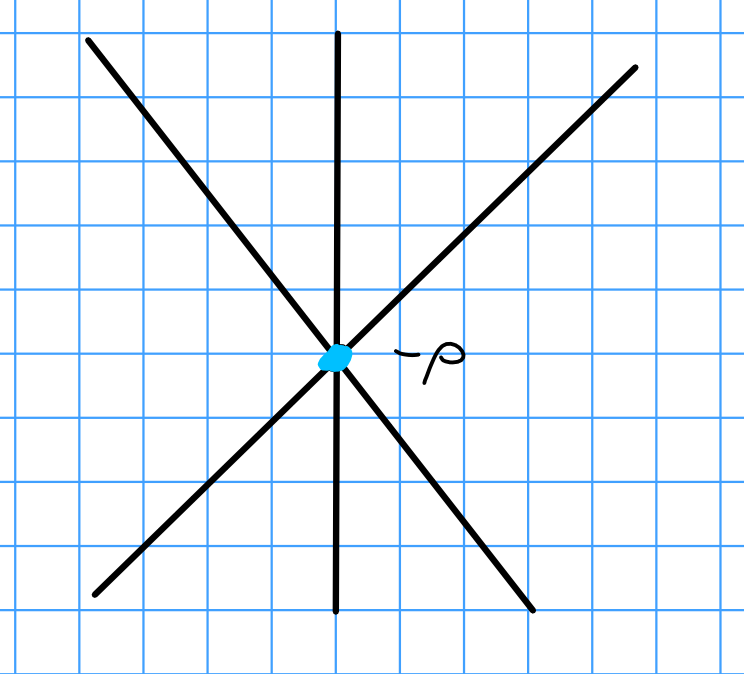
\includegraphics{figures/2020-02-05-09:26.png}\\

\begin{description}
\item[Proposition (Weights in Weyl Orbit Yield Equal Characters)]
If \(\lambda \in \Lambda\) and \(\mu \in W\cdot \lambda\), then
\(\chi_\mu = \chi_\lambda\).
\item[Proof]
Start with \(\alpha \in \Delta\) and consider
\(\mu = s_\alpha \cdot \lambda\). Since \(\lambda \in \Lambda\), we have
\(n\definedas (\lambda ,\alpha\dual) \in \ZZ\) by definition. There are
three cases:

\begin{enumerate}
\def\labelenumi{\arabic{enumi}.}
\item
  \(n\in \ZZ^+\), then \(M(s_\alpha \cdot \lambda) \subset M(\lambda)\).
  By Proposition 1.4, we have \(\chi_\mu =\chi_\lambda\).
\item
  For \(n=-1\),
  \(\mu = s_\alpha \cdot \lambda = \lambda + \rho -(\lambda + \rho, \alpha\dual)\alpha - \rho = \lambda + n+1 = \lambda + 0\).
  So \(\mu = \lambda\) and thus \(M_\mu = M_\lambda\).
\item
  For \(n\leq -2\),
\end{enumerate}

\begin{align*}
(\mu, \alpha\dual) 
&= (s_\alpha \cdot \lambda , \alpha\dual) \\
&= (\lambda i (n+1)\alpha, \alpha\dual) \\
&= n - 2(n+1) \\
&= -n-2 \\
&\geq 0
,\end{align*}

so
\(\chi_\mu = \chi_{s_\alpha \cdot \mu} = \chi_{s\alpha \cdot (s_\alpha \cdot \lambda)} = \chi_\lambda\).
Since \(W\) is generated by simple reflections and the linkage property
is transitive, the result follows by induction on \(\ell(w)\).
\item[Exercise (1.8)]
See book, show that certain properties of the dot action hold (namely
nonlinearity).
\end{description}

\hypertarget{extending-the-harish-chandra-morphism}{%
\subsection{1.9: Extending the Harish-Chandra
Morphism}\label{extending-the-harish-chandra-morphism}}

We want to extend the previous proposition from \(\lambda \in \Lambda\)
to \(\lambda \in \lieh\dual\). We'll use a density argument from affine
algebraic geometry, and switch to the Zariski topology on
\(\lieh\dual \subset \CC^n\).

Fix a basis \(\Delta = \theset{a_1, \cdots, a_\ell}\) and use the
Killing form to identify these with a basis for
\(\lieh = \theset{h_1, \cdots, h_\ell}\). Similarly, take
\(\theset{w_1, \cdots, w_\ell}\) as a basis for \(\lieh\dual\), and
we'll use the identification

\begin{align*}
\lieh\dual &\iff \AA^\ell \\
\lambda &\iff (\lambda(h_1), \cdots, \lambda(h_\ell))
.\end{align*}

We identify \(U(\lieh) = S(\lieh) = \CC[h_1, \cdots, h_\ell]\) with
\(P(\lieh\dual)\) which are polynomial functions on \(\lieh\dual\). Fix
\(\lambda \in \lieh\dual\), extended \(\lambda\) to be a multiplicative
function on polynomials. For \(f\in \CC[h_1, \cdots, h_\ell]\), we
defined \(\lambda(f)\). Under the identification, we send this to
\(\tilde f\) where \(\tilde f(\lambda) = \lambda(f)\).

\begin{quote}
Note: we'll identify \(f\) and \(\tilde f\) notationally going forward
and drop the tilde everywhere.
\end{quote}

Then \(W\) acts on \(P(\lieh\dual)\) by the dot action:
\((w\cdot \tilde f)(\lambda) = \tilde f(w\inv \cdot \lambda)\).

\begin{description}
\tightlist
\item[Exercise]
Check that this is a well-defined action.
\end{description}

Under this identification, we have

\begin{align*}
\lieh\dual &\iff \AA^\ell \\
\Lambda &\iff \ZZ^\ell
.\end{align*}

Note that \(\Lambda\) is discrete in the analytic topology, but is
\emph{dense} in the Zariski topology.

\begin{description}
\item[Proposition (Polynomials Vanishing on a Lattice Are Zero)]
A polynomial \(f\) on \(\AA^\ell\) vanishing on \(\ZZ^\ell\) must be
identically zero.
\item[Proof]
For \(\ell = 1\): A nonzero polynomial in one variable has only finitely
many zeros, but if \(f\) vanishes on \(\ZZ\) it has infinitely many
zeros.

For \(\ell > 1\): View \(f\in \CC[h_1, \cdots, h_{\ell-1}][h_\ell]\).
Substituting any fixed integers for the \(h_i\) for \(i\leq \ell - 1\)
yields a polynomial in one variable which vanishes on \(\ZZ\). By the
first case, \(f \equiv 0\), so the coefficients must all be zero and the
coefficient polynomials in \(\CC[h_1, \cdots ,h_{\ell-1}]\) vanish on
\(\ZZ^{\ell-1}\). By induction, these coefficient polynomials are
identically zero.
\item[Corollary (Lattices Are Zariski-Dense in Affine Space)]
The only Zariski-closed subset of \(\AA^\ell\) containing \(\ZZ^\ell\)
is \(\AA^\ell\) itself, so the Zariski closure
\(\bar{\ZZ^\ell} = \AA^\ell\) and \(\ZZ^\ell\) is dense in \(\AA^\ell\).
\end{description}

\hypertarget{friday-february-7th}{%
\section{Friday February 7th}\label{friday-february-7th}}

So far, we have \(\chi_\lambda = \chi_{w.\cdot \lambda}\) if
\(\lambda \in \Lambda\) and \(w\in W\). We have
\(\lieh\dual \supset \Lambda\) which is topologically equivalent to
\(\AA^\ell \supset \ZZ^\ell\), where \(\ZZ^\ell\) is dense in the
Zariski topology.

For \(z\in \mcz(\lieg)\), we have
\(\chi_\lambda(z) = \chi_{W\cdot \lambda} (z)\) and so
\(\lambda(\xi(z)) = (w\cdot \lambda )(\xi(z))\) where
\(\xi: \mcz(\lieg) \to U(\lieh) = S(\lieh) \cong P(\lieh\dual)\) where
we send \(\lambda(f)\) to \(f(\lambda)\).

Then \(\xi(z)(\lambda) = \xi(z)(w\cdot \lambda)\) for all
\(\lambda \in \Lambda\), and so \(\xi(z) = w\inv \xi(z)\) on
\(\Lambda\). But both sides here are polynomials and thus continuous,
and \(\Lambda \subset \lieh\dual\) is dense, so
\(\xi(z) = w\inv \xi(z)\) on all of \(\lieh\dual\). I.e.,
\(\chi_\lambda = \chi_{w\cdot } \lambda\) for all
\(\lambda \in \lieh\dual\).

This in fact shows that the image of \(\mcz(\lieg)\) under \(\xi\)
consists of \(W\dash\)invariant polynomials.

It's customary to state this in terms of the natural action of \(W\) on
polynomials without the row-shift. We do this by letting
\(\tau_\rho: S(\lieh) \mapsvia{\cong} S(\lieh)\) be the algebra
automorphism induced by \(f(\lambda) \mapsto f(\lambda - \rho)\). This
is clearly invertible by \(f(\lambda) \mapsto f(\lambda + \rho)\). We
then define
\begin{align*}\psi: \mcz(\lieg) \mapsvia{\xi} S(\lieh) \mapsvia{\tau_\rho} S(\lieh)\end{align*}
as this composition; this is referred to as the \textbf{Harish-Chandra}
(HC) homomorphism.

\begin{description}
\tightlist
\item[Exercise]
Show \(\chi_\lambda(z) = (\lambda + \rho) (\psi(z))\) and
\(\chi_{w\cdot \lambda} (w(\lambda+\rho))(\psi(z))\), where \(w(\wait)\)
is the usual \(w\dash\)action.
\end{description}

Replacing \(\lambda\) by \(\lambda + \rho\) and \(w\) by \(w\inv\), we
get
\begin{align*}
w\psi(z) = \psi(z)
\end{align*} for all \(z\in \mcz(\lieg)\) and all \(w\in W\) where
\((w\psi(z))(\lambda) = \psi(z)(w\inv \lambda)\).

We've proved that

\begin{description}
\item[Theorem (Character Linkage and Image of the HC Morphism)]
\hfill

\begin{enumerate}
\def\labelenumi{\alph{enumi}.}
\item
  If \(\lambda, \mu \in \lieh\dual\) that are linked, then
  \(\chi_\lambda = \chi_\mu\).
\item
  The image of the twisted HC homomorphism
  \(\psi: \mcz(\lieg) \to U(\lieh) = S(\lieh)\) lies in the subalgebra
  \(S(\lieh)^W\).
\end{enumerate}
\item[Example]
Let \(\lieg = \liesl_2\). Recall from finite-dimensional representations
there is a canonical element \(c\in \mcz(\lieg)\) called the Casimir
element. For \(\OO\), we need information about the full center
\(\mcz(\lieg)\) (hence introducing infinitesimal characters).

Expressing \(c\) in the PBW basis yields \(c = h^2 + 2h + 4yx\), where
\(h^2 + 2h \in U(\lieh)\) and
\(4yx \in \lien^- U(\lieg) + U(\lieg) \lien\).

\begin{quote}
Enveloping algebra convention: \(x\)s, \(h\)s, \(y\)s
\end{quote}

Then \(\xi(c) = \pr(c) = h^2 + 2h\), and under the identification
\(\lieh\dual \iff \CC\) where \(\lambda \iff \lambda(h)\), we can
identify \(\rho \iff \rho(h) = 1\). The row shift is given by
\(\psi(c) = (h-1)^2 + 2(h-1) = h^2 - 1\). This is \(W\dash\)invariant,
since \(s_{\alpha_h} = -h\). But \(W = \generators{s_\alpha, 1}\), so
\(s_\alpha\) generates \(W\).

We also have
\(\chi_\lambda(c) = (\lambda + \rho) (\psi(c)) = (\lambda+1)^2 - 1\).
Then
\begin{align*}
\chi_\lambda(c) = \chi_\mu(c) \iff (\lambda+1)^2 - 1 = (\mu + 1)^2 \iff \mu = \lambda \text{ or } \mu = -\lambda - 2
\end{align*}

But \(\lambda = 1 \cdot \lambda\) and
\(-\lambda - 2 = s_\alpha \cdot \lambda\), so
\(\mcz(\lieg) = \generators{c} \definedas \CC[c]\) as an algebra. So
these characters are equal iff \(\mu = w\cdot \lambda\) for \(w\in W\).
\end{description}

\hypertarget{section-1.10-harish-chandras-theorem}{%
\section{Section 1.10: Harish-Chandra's
Theorem}\label{section-1.10-harish-chandras-theorem}}

Goal: prove the converse of the previous theorem.

\begin{description}
\item[Theorem (Harish-Chandra)]
Let \(\psi: \mcz(\lieg) \to S(\lieh)\) be the twisted HC homomorphism.
Then

\begin{enumerate}
\def\labelenumi{\alph{enumi}.}
\item
  \(\psi\) is an \emph{isomorphism} of \(\mcz(\lieg)\) onto
  \(S(\lieh)^W\).
\item
  For all \(\lambda, \mu \in \lieh\dual\), \(\chi_\lambda = \chi_\mu\)
  iff \(\mu = w\cdot \lambda\) for some \(w\in W\).
\item
  Every central character \(\chi: \mcz(\lieg) \to \CC\) is a
  \(\chi_\lambda\).
\end{enumerate}
\item[Proof (of (a))]
Relies heavily on the \emph{Chevalley Restriction Theorem} (which we
won't prove here).

Initially we have a restriction map on polynomial functions
\(\theta: P(\lieg) \to P(\lieh)\). We identified
\(P(\lieg) = S(\lieg\dual)\), the formal polynomials on \(\lieg\dual\).
However, for \(\lieg\) semisimple, we can identify
\(S(\lieg\dual) \cong S(\lieg)\) via the Killing form.

By the Chinese Remainder Theorem, \(\theta: S(\lieg)^G \to S(\lieh)^W\)
is an isomorphism, where the subgroup \(G \leq \aut(\lieg)\) is the
\emph{adjoint group} generated by
\(\theset{\exp \ad_x \suchthat x \text{ is nilpotent}}\).

It turns out that \(S(\lieg)^G\) is very close to \(\mcz(\lieg)\) -- it
is the associated graded of a natural filtration on \(\mcz(\lieg)\).
This is enough to show that \(\psi\) is a bijection.
\item[Proof (of (b))]
We'll prove the contrapositive of the converse.

Suppose \(W\cdot \lambda \intersect W\cdot \mu = \emptyset\) and both
are in \(\lieh\dual\). Since these are finite sets, Lagrange
interpolation yields a polynomial that is 1 on \(W\cdot \lambda\) and 0
on \(W\cdot \mu\). Let \(g = \frac{1}{\abs W} \sum_{w\in W} w\cdot f\).

\begin{quote}
Note: definitely the dot action here, may be a typo in the book.
\end{quote}

Then \(g\) is a \(W\cdot\) invariant polynomial with the same
properties. By part (a), we can get rid of the row shift to obtain an
isomorphism \(\xi: \mcz(\lieg) \to S(\lieh)^(W\cdot)\), the \(W\cdot\)
invariant polynomials. Choose \(z\in \mcz(\lieg)\) such that
\(\xi(z) = g\), then
\(\chi_\lambda(z) = \lambda(\xi(z)) = \lambda(g) = g(\lambda) = 1\). So
\(\chi_\mu(z) = 0\) similarly, and \(\chi_\lambda = \chi_\mu\).
\item[Proof (of (c))]
This follows from some commutative algebra, we won't say much here. Look
at maximal ideals in \(\CC[x, y,\cdots]\) which correspond to evaluating
on points in \(\CC^\ell\).
\end{description}

\(\qed\)

\begin{description}
\tightlist
\item[Remark]
Chevalley actually proved that
\(S(\lieh)^W \cong \CC(p_1, \cdots, p_\ell)\) where the \(p_i\) are
homogeneous polynomials of degrees \(d_1 \leq \cdots \leq d_\ell\).
These numbers satisfy some remarkable properties:
\(\prod d_i = \abs{W}\) and \(d_1 = 2\) (these are called the
\emph{degrees of \(W\)})
\end{description}

\hypertarget{section-1.11}{%
\section{Section 1.11}\label{section-1.11}}

\begin{description}
\tightlist
\item[Theorem (Category O is Artinian)]
Category \(\OO\) is \emph{artinian}, i.e.~every \(M \in \OO\) is
Artinian (DCC) and \(\dim \hom_\lieg(M, N) < \infty\) for every
\(M, N\).
\end{description}

Recall that \(\OO\) is known to be Noetherian from an earlier theorem.
This will imply that \textbf{every \(M\) has a composition/Jordan-Holder
series}, so we can take composition factors and multiplicities.

Most interesting question: what are the factors/multiplicities of the
simple modules and Verma modules?

\hypertarget{wednesday-february-12th}{%
\section{Wednesday February 12th}\label{wednesday-february-12th}}

\hypertarget{infinitesimal-blocks}{%
\subsection{Infinitesimal Blocks}\label{infinitesimal-blocks}}

We'll break up category \(\OO\) into smaller subcategories (blocks).

Recall theorem 1.1 (e): \(\mcz(\lieg)\) acts locally finitely on
\(M\in \OO\), and \(M\) has a \emph{finite} filtration with highest
weight sections, so \(M\) should involve only a finite number of central
characters \(\chi_\lambda\) (where \(\lambda \in\lieh\dual\)).

\begin{quote}
Note: an analog of Jordan decomposition works here because of this
finiteness condition. This discussion will parallel the JCF of a simple
operator on a finite dimensional \(\CC\dash\)vector space. However, this
involves the \emph{entire} center instead of just scalar matrices, so
the analogy is diagonalizing a family of operators simultaneously.
\end{quote}

Let \(\chi \in \hat \mcz(\lieg)\) and \(M\in \OO\), and
\begin{align*}
M^\chi \definedas \theset{v\in M \suchthat ~\forall z\in \mcz(\lieg),~\exists n>0 \st (z- \chi(z))^n \cdot v = 0}
\end{align*}

Idea: write
\begin{align*}
z = \chi(z) \cdot 1 + (z-\chi(z)\cdot 1),
\end{align*} where the first is a scalar operator and the second is
(locally) nilpotent on \(M^\chi\). Thus we can always arrange for \(z\)
to act by a sum of ``Jordan blocks'':

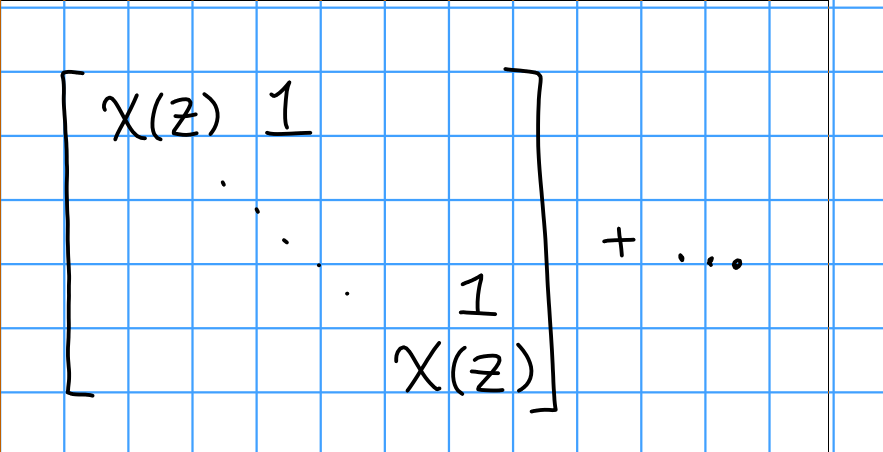
\includegraphics{figures/2020-02-12-09:15.png}\\

Some observations:

\begin{itemize}
\tightlist
\item
  \(M^\chi\) are \(U(\lieg)\dash\)submodules of \(M\).
\item
  The subspaces \(M^\chi\) are linearly independent
\item
  \(\mcz(\lieg)\) stabilizes each \(M_\mu\) since \(\mcz(\lieg)\) and
  \(U(\lieh)\) are a commuting family of operators on \(M_\mu\).
\item
  We can write
  \begin{align*}M_\mu = \bigoplus_{\chi \in \hat\mcz(\lieg)} (M_\mu \intersect M^\chi),\end{align*}
  and since \(M\) is generated by a finite sum of weight spaces,
  \(M = \bigoplus_{\chi \in \hat\mcz(\lieg)} M^\chi\).
\item
  By Harish-Chandra's theorem, every \(\chi\) is \(\chi_\lambda\) for
  some \(\lambda \in \lieh\dual\).
\end{itemize}

Let \(\OO_\chi\) be the full subcategory of modules \(M\) such that
\(M = M^\chi\); we refer to this as a \emph{block}.

\begin{quote}
Note: full subcategory means keep all of the hom sets.
\end{quote}

\begin{description}
\tightlist
\item[Proposition (O Factors into Blocks, Indecomposables/Highest Weight
Modules Lie in a Single Block)]
\(\OO = \bigoplus_{\lambda \in \lieh\dual} \OO_{\chi_\lambda}\). Each
indecomposable module in \(\OO\) lies in a \emph{unique} \(\OO_\chi\).
In particular, any highest weight module of highest weight \(\lambda\)
lies in \(\OO_{\chi_\lambda}\).
\end{description}

Thus we can reduce to studying \(\OO_{\chi_\lambda}\).

\emph{Remark:} \(\OO_{\chi_\lambda}\) has a finite number of simple
modules \(\theset{L(w\cdot \lambda) \suchthat w\in W}\) and a finite
number of Verma modules \(\theset{M(w\cdot \lambda) \suchthat w\in W}\).

\hypertarget{blocks}{%
\subsection{Blocks}\label{blocks}}

Let \(\mcc\) be a category with is artinian and noetherian, with
\(L_1, L_2\) simple modules. We say \(L_1 \sim L_2\) if there exists a
non-split extension
\begin{align*}0 \to L_1 \to M \to L_2 \to 0,\end{align*}
i.e.~\(\ext^1_\OO(L_2, L_1) \neq 0\). In particular, \(M\) equivalently
needs to be indecomposable. We then extend \(\sim\) to be
reflexive/symmetric/transitive to obtain an equivalence relation.

\begin{quote}
\(L_1\) ends up being the socle here.
\end{quote}

This partitions the simple modules in \(\mcc\) into \emph{blocks}
\(\mcb\). More generally, we say \(M\in \mcc\) belongs to \(\mcb\) iff
all of the composition factors of \(M\) belong to \(\mcb\). Although not
obvious, there are no nontrivial extensions between modules in different
blocks. Thus each simple module (generally, just an object)
\(M\in \mcc\) decomposes as a direct sum of submodules (subobjects) with
each belonging to a single block.

\emph{Question:} Is \(\OO_\chi\) a block of \(\OO\)? The answer is not
always. Because each indecomposable module in \(\OO\) lives in a simple
\(\OO_\chi\) By the definition, it's clear that each block is contained
in a single simple infinitesimal block \(\OO_\chi\).

\begin{quote}
The block containing \(L_1, L_2\) will be contained in the same
infinitesimal block, and continuing the composition series puts all
composition factors in a single block.
\end{quote}

\begin{description}
\item[Proposition (Integral Weights Yield Simple Blocks)]
If \(\lambda\) is an \emph{integral} weight, so \(\lambda \in \Lambda\),
then \(\OO_{\chi_\lambda}\) is a (simple) block of \(\OO\).
\item[Proof]
It suffices to show that all \(L(w\cdot \lambda)\) for \(w\in W\) lie in
a single block. We'll induct on the length of \(w\). Start with
\(2 = s_\alpha\) for some \(\alpha\in \Delta\). Let
\(\mu = s_\alpha \cdot \lambda\). If \(\mu = \lambda\), i.e.~\(\lambda\)
is in the stabilizer, then we're done.

Otherwise, assume WLOG \(\mu < \lambda\) in the partial order, using the
fact that \(\lambda \in \Lambda\). (The difference between these is just
an integer multiple of \(\alpha\).)

By proposition 1.4, we have the following maps:

\begin{center}
\begin{tikzcd}
M(\mu) \arrow[rr, "\phi\neq 0"]           &  & N(\lambda) \arrow[rr, hook]       &  & M(\lambda) \\
                                          &  &                                   &  &            \\
N(\mu) \arrow[rr, tail] \arrow[uu, hook]  &  & N = \phi(N(\mu)) \arrow[uu, hook] &  &           
\end{tikzcd}
\end{center}

Then \(\phi\) induces a map \(L(\mu) \mapsvia{\bar \phi} M(\lambda)/N\),
where the codomain here is a highest weight module with quotient
\(L(\lambda)\). Since highest weight modules are indecomposable and thus
lie in a single bloc, \(L(\mu)\) and \(L(\lambda)\) are in the same
block.

\begin{quote}
Note that if \(v^+\) generates \(M(\lambda)\), \(v^+ + N\) generated the
quotient.
\end{quote}

Now inducting on \(\ell(w)\), iterating this argument yields all
\(L(w\cdot \lambda)\) (as \(w\) varies) in the same block.
\item[Example]
This isn't true for non-integral weights. Let \(\lieg = \liesl(2, \CC)\)
with \(\lambda \in \RR \setminus \ZZ\) and \(\lambda > -1\). Then

\begin{align*}
\mu 
&= s_\alpha \lambda  \\
&= -\lambda - 2  \\
&<_{\RR} -1
\end{align*}

with the usual ordering on \(\RR\), but \(\mu \not > \lambda\) in the
ordering on \(\lieh\dual\): we have \(\lambda - \mu = 2\lambda + 2\),
but \(\alpha \equiv 2\) and thus these don't differ by an element of
\(2\ZZ\).

Thus \(\mu, \lambda\) are in different cosets of \(\ZZ\Phi = \Lambda_r\)
in \(\lieh\dual\). However, \(M(\lambda), M(\mu)\) are simple since
\(\lambda, \mu\) are not non-negative integers.

By exercise 1.13, there can be no nontrivial extension, so they're in
different homological blocks but in the same \(\OO_{\chi_\lambda}\)
since \(\mu = s_\alpha \cdot \lambda\). So this infinitesimal block
splits into multiple homological blocks.
\end{description}

Friday: 1.14 and 1.15.

\hypertarget{friday-february-14th}{%
\section{Friday February 14th}\label{friday-february-14th}}

Recall that we have a decomposition
\begin{align*}\OO = \bigoplus_{\chi \in \hat\mcz(\lieg)} \OO_\chi\end{align*}
into infinitesimal blocks, where \(\OO_0 \definedas \OO_{\chi_0}\) is
the principal block. Since \(0\in\lieh\dual\), we can associate
\(\chi_0, M_0, L(0) = \CC\) the trivial module for \(\lieg\).

\hypertarget{formal-characters}{%
\subsection{1.14 -- 1.15: Formal Characters}\label{formal-characters}}

Some background from finite dimensional representation theory of a
finite group \(G\) over \(\CC\). The hope is to find matrices for each
element of \(G\), but this isn't basis invariant. Instead, we take
traces of these matrices, which is less data and basis-independent This
is referred to as the \emph{character} of the representation, and in
nice situations, the characters determine the irreducible
representations.

For a semisimple lie algebra \(\lieg\) and a finite dimensional
representation \(M\), it's enough to keep track of weight multiplicities
when \(\lieg\) is the lie algebra associated to a compact lie group
\(G\). From this data, the characters can be recovered. So the data of
all pairs \((\dim M_\lambda, \lambda \in \lieh\dual)\) suffices. To
track this information, we introduce a \emph{formal character}.

\emph{Remark:} If \(G\) is a group and \(k\) is a commutative ring,
\(kG\) is the group ring of \(G\). This has the following properties:

\begin{itemize}
\tightlist
\item
  \(\sum a_i g_i + \sum b_i g_i = \sum(a_i + b_i) g_i\)
\item
  \(\qty{ \sum a_i g_i } \qty{ \sum b_i g_i } = \sum_{i, j} a_i b_j g_i g_j\)
\end{itemize}

Let \(\ZZ \Lambda\) be the integral group ring of the lattice. Since
\(\Lambda\) is an abelian group, and the additive notation would be more
difficult. So we write \(\Lambda\) multiplicatively and introduce
\(e(\lambda)\) for \(\lambda \in \lieh\dual\), where
\(e(\lambda) e(\mu) = e(\lambda + \mu)\). For \(M\) a finite dimensional
\(\lieg\dash\)module, the formal character of \(M\) is given by

\begin{align*}
\ch M = \sum_{\lambda\in \Lambda} \qty{ M(\lambda)  } e(\lambda) \quad\in \ZZ\Lambda
.\end{align*}

This satisfies

\begin{itemize}
\tightlist
\item
  \(\ch(M\oplus N) = \ch(M) + \ch(N)\)
\item
  \(\ch(M\tensor N) = \ch(M)\ch(N)\)
\item
  For \(\ch(M) = \sum a_\mu e(\mu)\) and \(\ch(N) = \sum b_\nu e(\nu)\),
  we have
  \begin{align*}\ch(M) \ch(N) = \sum_{\lambda} \qty{ \sum_{\mu + \nu = \lambda} a_\mu b_\nu } e(\lambda)\end{align*}
\end{itemize}

By Weyl's complete reducibility theorem, any semisimple module
decomposes into a sum of simple modules. Thus it suffices to determine
that characters of simple modules \(L(\lambda)\) for
\(\lambda \in \Lambda^+\), corresponding to dominant integral weights.
Then we can reconstruct \(\ch(M)\) from \(\ch L(\lambda)\) for
\(M\in \OO\).

Specifying the weight spaces dimensions is equivalent to a function
\(\ch_M: \lieh\dual \to \ZZ^+\) where
\(\ch_M(\lambda) = \dim M_\lambda\). The analogy of \(e(\lambda)\) in
this setting is the characteristic function \(e_\lambda\) where
\(e_\lambda(\mu) = \delta_{\lambda \mu}\) for \(\mu \in \lieh\dual\). We
can thus write the function

\begin{align*}
\ch_M = \sum_{\lambda \in \lieh\dual} \qty{ \dim M_\lambda } e_\lambda
.\end{align*}

When \(\dim M < \infty\), \(\ch_M\) has finite support, although we
generally don't have this in \(\OO\). In this setting, multiplication of
formal characters corresponds to convolution of functions, i.e.~
\begin{align*}(f\ast g)(\lambda) = \sum_{\mu + \nu = \lambda} f(\mu) g(\nu).\end{align*}
Define
\begin{align*}
\mcx = \theset{f: \lieh\dual \to \ZZ \suchthat \supp(f) \subset \union_{i\leq n} \qty{ \lambda_i - \ZZ^+ \Phi^+  }  ~~\text{ for some } \lambda_1, \cdots, \lambda_n \in \lieh\dual }
\end{align*}

\begin{quote}
Idea: this is a ``cone'' below some weights.
\end{quote}

This makes \(\mcx\) into a \(\ZZ\dash\)module with a well-defined
convolution, thus \(\mcx\) is a commutative ring where

\begin{itemize}
\tightlist
\item
  \(e_\lambda \in \mcx\) for all \(\lambda\)
\item
  \(e_0 = 1\)
\item
  \(e_\lambda \ast e_\mu = e_{\lambda + \mu}\).
\end{itemize}

If \(M\in \OO\), then \(\ch_M \in \mcx\) by axiom O5 (local finiteness).

\emph{Example:}
\(\ch L(\lambda) = e(\lambda) + \sum_{\mu < \lambda} m_{\lambda \mu} e(\mu)\),
where \(m_{\lambda \mu} = \dim L(\lambda)_{\mu} \in \ZZ^\pm\).

\begin{description}
\item[Definition (Principal Block)]
Let \(\mcx_0\) be the additive subgroup of \(\mcx\) generated by all
\(\ch M\) for \(M \in \OO\).
\item[Proposition (Additivity of Characters, Correspondence with K(O) )]
\hfill

\begin{enumerate}
\def\labelenumi{\alph{enumi}.}
\item
  If \(0 \to M' \to M \to M'' \to 0\) is a SES in \(\OO\), then
  \(\ch M = \ch M' + \ch M''\).
\item
  There is a 1-to-1 correspondence
\end{enumerate}

\begin{align*}
\mcx_0 &\iff K(\OO) \\
\ch M &\iff [M]
,\end{align*}

where \(K\) is the Grothendieck group.

\begin{enumerate}
\def\labelenumi{\alph{enumi}.}
\setcounter{enumi}{2}
\tightlist
\item
  If \(M\in \OO\) and \(\dim L < \infty\), then
  \(\ch(L\tensor M) = \ch L \ast \ch M\).
\end{enumerate}
\end{description}

\emph{Remark:} (a) implies that \(\ch M\) is the sum of the formal
characters of its composition factors with multiplicities. Thus
\begin{align*}
\ch M = \sum_{L \text{ simple }} [M:L] ~\ch L
.\end{align*}

\begin{description}
\tightlist
\item[Proof (of a)]
Use the fact that
\(\dim M_\lambda = \dim M_\lambda' + \dim M_\lambda''\)
\item[Proof (of b)]
Check that the obvious maps are well-defined and mutually inverse.
\item[Proof (of c)]
Because of the module structure we've put on the tensor product
\((L \tensor M)_\lambda = \sum_{\mu + \nu = \lambda} L_\mu \tensor M_\nu\).
\end{description}

\emph{Remark:} The natural action of \(W\) on \(\Lambda\) or on
\(\lieh\dual\) extends to \(\ZZ \Lambda\) and \(\mcx\) if we define

\begin{align*}
w\cdot e(\lambda) \definedas e(w\lambda) \quad w\in W,~~\lambda \in \Lambda \text{ or } \lieh\dual
.\end{align*}

If \(\lambda \in \Lambda^+\), then
\(w( \ch L(\lambda) ) = \ch L(\lambda)\) since
\(\dim L(\lambda)_\mu = \dim L(\lambda)_{w\mu}\). Thus the characters of
simple finite-dimensional modules are \(W\dash\)invariant.

\hypertarget{formal-characters-of-verma-modules}{%
\subsection{1.16: Formal Characters of Verma
Modules}\label{formal-characters-of-verma-modules}}

1: We have a similar formula

\begin{align*}
\ch M(\lambda) = \ch L(\lambda) + \sum_{\mu < \lambda} a_{\lambda \mu} \ch L(\mu) \\
\quad \text{ with } a_{\lambda \mu} \in \ZZ^+ 
\text{ and } a_{\lambda \mu} = [M(\lambda): L(\mu)]
.\end{align*}

This all happens in a single block of \(\OO\), which has finitely many
simple and Verma modules.\\
In fact, the sum will be over
\(\theset{ \mu \in W\cdot \lambda \suchthat \mu < \lambda}\). But
computing \(L(\mu)\) is difficult in general.

Since the set of weights \(W\cdot \lambda\) is finite, we can totally
order it in a way that's compatible with the partial order on
\(\lieh\dual\) (so \(\leq\) in the partial order implies \(\leq\) in the
total order). So if we order the weights \(\mu_i\) indexing the Verma
modules in columns and indexing the simple modules in the rows, this is
an upper triangular matrix with 1s on the diagonal. This can inverted
since it's unipotent, with the inverse of same upper triangular form.

2: We can write
\begin{align*}
\ch L(\lambda) 
= \ch M(\lambda) + 
\sum_{\mu < \lambda,~\mu \in W\cdot \lambda} b_{\lambda \mu} \ch M(\mu) \quad b_{\lambda \mu} \in \ZZ
\end{align*} This expresses the character in terms of Verma modules,
which are easier to compute.

Next time: formulas for the characters

\hypertarget{monday-february-17th}{%
\section{Monday February 17th}\label{monday-february-17th}}

\hypertarget{character-formulas}{%
\subsection{Character Formulas}\label{character-formulas}}

\emph{Last time:} The second character formula (equation (2)),

\begin{align*}
\ch L(\lambda) =  \ch M(\lambda) + \sum_{\mu < \lambda, ~~ \mu \in W\cdot \lambda} b_{\lambda, \mu} ~\ch M(\mu)
.\end{align*}

Note that \(b_{\lambda, \mu} \in \ZZ\), and this formula comes from
inverting the previous one.

\begin{quote}
Holy grail: characters of simple modules!
\end{quote}

We can write \(M(\lambda) \cong U(\lien^-) \tensor_\CC \CC_\lambda\) as
a \(\lieh\dash\)module. Define \(p: \lieh\dual \to \ZZ\) where
\(p(\gamma)\) is the number of tuples \((t_\beta)_{\beta\in\Phi^+}\)
where \(t_\beta \in \ZZ^+\) and
\(\gamma = - \sum_{\beta \in \Phi^+} t_\beta \beta\). We have
\(\supp(p) = - \ZZ^+ \Phi^+\), which gives us something like a negative
quadrant of the lattice.

The function \(p\) is essentially the \emph{Kostant partition function}.
The advantage here is that \(p \in \mcx\) (defined last time, support is
less than some finite weights?).

\emph{Observation:} \(p = \ch_{M(0)}\) since
\(U(\lien^-) \tensor \CC_{\lambda = 0}\) has PBW basis
\begin{align*}
\theset{ \prod_{\beta\in\Phi^+} y_\beta^{t_\beta} \tensor 1_{\lambda = 0} \suchthat t_\beta \in \ZZ^+ }.
\end{align*}

\emph{Example:} Let \(\lieg = \liesl(3)\), then
\(\Phi^+ = \theset{\alpha_1, \alpha_2, \alpha_1 + \alpha_2}\). Then
\(\gamma = -\qty{\alpha_1 + 2\alpha_2}\) corresponds to
\((1,2,0), (0,1,1)\) so \(p(\gamma) = 2\). If
\(\gamma = -\qty{2\alpha_1 + 2\alpha_2}\), this corresponds to
\((2,2,0), (1,1,1), (0,0,2)\) so \(p(\gamma) = 3\).

\begin{quote}
Note: just the number of ways of obtaining \(-\gamma\) as a linear
combinations of roots.
\end{quote}

In general, \(\dim M(0)_\gamma = p(\gamma)\).

\begin{description}
\tightlist
\item[Proposition (Characters as Convolution Products)]
For any \(\lambda \in \lieh\dual\), we have
\(\ch_{M_\lambda} = p\ast e_\gamma\), taking the convolution product.
\end{description}

In particular, \(\ch_{M(0)} = p\).

\begin{description}
\tightlist
\item[Proof (of Proposition)]
We have the following computation: \begin{align*}
(p\ast e_\lambda)(\lambda+\gamma)
&= p(\gamma) e_\lambda(\lambda) \\
&= p(\gamma) 1 \\
&= p(\gamma) \\
&= \dim M(\lambda)_{\lambda + \gamma} \quad\text{ as a weight space }
.\end{align*}
\end{description}

Note that we can also write equation (2) as

\begin{align*}
\ch L(\lambda) = \sum_{w\cdot \lambda \leq \lambda} b_{\lambda, w} \ch M(w\cdot \lambda)
.\end{align*}

Here \(b_{\lambda, w} \in \ZZ\) and in fact \(b_{\lambda, 1} = 1\).

\emph{Example:} Let \(\lieg = \liesl(2)\). We know

\begin{align*}
\ch M(\lambda) &= \ch L(\lambda) + \ch L(s_\alpha \cdot \lambda) \\
\ch M(s_\alpha \cdot \lambda) &= \ch L(s_\alpha \cdot \lambda)
.\end{align*}

We can think of this pictorially as the `head' on top of the socle:

\begin{align*}
M(\lambda) = \frac{L(\lambda)}{L(s_\alpha \cdot \lambda)}
.\end{align*}

The formula above corresponds to the matrix
\begin{align*}
\left[\begin{array}{cc} 1 & 1 \\ 0 & 1 \end{array}\right]
\end{align*}

We can invert the formula to get equation (2), which corresponds to
inverting this matrix:

\begin{align*}
\ch L(\lambda) &= \ch M(\lambda) - \ch M(s_\alpha \cdot \lambda) \\
\ch L(s_\alpha \cdot \lambda) &= \ch M(s_\alpha \cdot \lambda)
.\end{align*}

Note that the coefficients \(b_{w, \lambda} \in \theset{0, \pm 1}\) in
this equation are independent of \(\lambda \in \Lambda^+\).

If \(\lambda \not\in\Lambda^+\), then
\(\ch L(\lambda) = \ch M(\lambda)\) and
\(b_{\lambda, 1} = 1, b_{\lambda, s_\alpha} = 0\) are again independent
of \(\lambda \in \lieh\dual \setminus \Lambda^+\).

\textbf{Question:} To what extent to \(b_{\lambda, w}\) depend on
\(\lambda\)? The answer is seemingly ``not much''.

\hypertarget{category-oo-methods}{%
\subsection{\texorpdfstring{Category \(\OO\)
Methods}{Category \textbackslash OO Methods}}\label{category-oo-methods}}

\begin{quote}
Note: skipping chapter 2 since we're focusing on infinite dimensional
representations.
\end{quote}

\hypertarget{hom-and-ext}{%
\subsubsection{Hom and Ext}\label{hom-and-ext}}

Recall that \(\hom(\wait, \wait)\) is left exact but not exact, and is
either covariant or contravariant depending on which variable is fixed.
So taking \(\hom\) of a SES yields a LES involving the derived functors
\(\ext^n\). Convention: \(\ext^0 \definedas \hom\) and
\(\ext^1 \definedas \ext\).

Let \(A, C\) be \(U(\lieg)\dash\)modules. Consider two short exact
sequences

\begin{align*}
0 &\to A \to B \to C \to 0 \\
0 &\to A \to B' \to C \to 0
.\end{align*}

where \(B, B'\) are extensions of \(C\) by \(A\).

We say two such sequences are equivalent iff there is an isomorphism
making this diagram commute:

\begin{center}
\begin{tikzcd}
                        & B \arrow[rd] \arrow[dd, "\cong"] &   \\
A \arrow[rd] \arrow[ru] &                                  & C \\
                        & B' \arrow[ru]                    &
\end{tikzcd}
\end{center}

The set \(\ext_{U(\lieg)}(C, A)\) of equivalence classes of extensions
is a group under an operation called ``Baer sum'' (see Wikipedia) in
which the identity is the class of the split SES
\begin{align*}
0 \to A \to A\oplus C \to C \to 0.
\end{align*}

It turns out that the first right-derived functor of \(\hom\) defined
using projective resolutions, namely \(\ext_1\), is isomorphic to
\(\ext\). In particular, each SES leads to a pair of LESs given by
applying \(\hom(\wait, D)\) and \(\hom(E, \wait)\) for
\(D, E \in U(\lieg)\dash\)mod.

\textbf{Warning:} Even if \(A, C\in \OO\), there's no guarantee
\(B\in \OO\) for \(B\) an extension. In this case, we define
\(\ext_\OO(C, A)\) to be only those extensions lying in \(\OO\).

\begin{description}
\item[Proposition (Homs and Exts for Vermas and Quotients)]
Let \(\lambda, \mu \in \lieh\dual\).

\begin{enumerate}
\def\labelenumi{\alph{enumi}.}
\item
  If \(M\) is a highest weight module of highest weight \(\mu\) and
  \(\lambda \not< \mu\), then \(\ext_\OO(M(\lambda), M) = 0\).
  Contrapositive: nontrivial extensions force the strict inequality
  \(\mu < \lambda\). In particular, \(\ext_\OO(M(\lambda), X) = 0\) for
  \(X = L(\lambda), M(\lambda)\).
\item
  If \(\mu \leq \lambda\), then \(\ext_\OO(M(\lambda), L(\mu)) = 0\).
\item
  If \(\mu < \lambda\), then
  \(\ext_\OO(L(\lambda), L(\mu)) \cong \hom_\OO(N(\lambda), L(\mu))\).

  \begin{quote}
  \begin{enumerate}
  \def\labelenumii{(\alph{enumii})}
  \setcounter{enumii}{2}
  \tightlist
  \item
    is useful, homs can be easier to compute. Can just look at radical
    structure of \(N\), i.e.~just the head.
  \end{enumerate}
  \end{quote}
\item
  \(\ext_\OO(L(\lambda), L(\lambda)) = 0\).
\end{enumerate}
\item[Proof (of (a))]
Given an extension
\(0 \to M \mapsvia{f} E \mapsvia{g} M(\lambda) \to 0\) where \(M\) is a
highest weight module of highest weight \(\mu \not< \lambda\). We want
to show it splits.

\emph{Claim:} Let \(v^+\) be a maximal vector of \(M(\lambda)\), let
\(v\) be its preimage under \(g\), then \(v\) is a maximal vector of
weight \(\lambda\) in \(E\). For \(x\in \lien\), we can think of the RHS
as a quotient and identify

\begin{align*}
x\cdot v + M
&= x\cdot (v+M) \\
&= x\cdot v^+ \\
&= 0 \\
&= 0 + M
,\end{align*}

and for these to be equal this implies \(x\cdot v \in M\). But
\(x\cdot v\) has weight \(> \lambda\); since \(\mu \not> \lambda\),
\(M\) has no such weights. So we must have \(x\cdot v = 0\in E\), and
\(v\) is a maximal vector.

It's also the case that \(U(\lien^-)\) acts freely on \(v\), since it
acts freely on its image in the quotient \(M(\lambda)\). So \(v\)
generates a submodule \(\generators{v} \leq E\) isomorphic to
\(M(\lambda)\). This defines a splitting (because of the freeness of
this action) given by \(h(v^+) = v\).
\item[Proof (of (b))]
Follows from (a).
\item[Proof (of (c))]
Look at the SES \(0\to N(\lambda) \to M(\lambda) \to L(\lambda) \to 0\).
Apply \(\hom_\OO(\wait, L(\mu))\) to get the LES

\begin{align*}
\cdots &\to \hom_\OO(M(\lambda), L(\mu)) \to \hom_\OO( N(\lambda), L(\mu)  ) \\
&\to \ext_\OO( L(\lambda), L(\mu)  ) \to \ext_\OO( M(\lambda), L(\mu)  ) \to \cdots
\end{align*}

and since \(L(\lambda)\) is the only simple quotient of \(M(\lambda)\),
so the first \(\hom\) is zero. Similarly, the last \(\ext_\OO\) is zero
by (b), and the middle is an isomorphism.
\item[Proof (of (d))]
Replace \(\mu\) by \(\lambda\) in the LES, now term 2 above is zero
since \(\Pi(L(\lambda)) < \lambda\). Term 4 is zero by (b), and thus
term 3 is zero.
\end{description}

Next section: duality in category \(\OO\).

\hypertarget{monday-february-24th}{%
\section{Monday February 24th}\label{monday-february-24th}}

\hypertarget{antidominant-weights}{%
\subsection{Antidominant Weights}\label{antidominant-weights}}

Recall that for \(\lambda \in \lieh\dual\), we can associate
\(\Phi_{[\lambda]}\) and \(W_{[\lambda]}\) and consider
\(W_{[\lambda]} \cdot \lambda\). When \(\lambda \in \Lambda\) is
integral and \(\mu \in W\lambda \intersect \Lambda^+\), we have
\(M(\mu) \to L(\mu)\) its simple quotient, which is finite-dimensional.

\begin{description}
\tightlist
\item[Definition (Antidominant)]
\(\lambda \in \lieh\dual\) is \emph{antidominant} if
\((\lambda + \rho, \alpha\dual) \not\in \ZZ^{> 0}\) for all
\(\alpha \in \Phi^+\). Dually, \(\lambda\) is \emph{dominant} if
\((\lambda + \rho, \alpha\dual)\not\in\ZZ^{<0}\) for all
\(\alpha\in\Phi^+\).
\end{description}

Note that most weights are both dominant and antidominant. Example: take
\(\lambda = -\rho\). We won't use the dominant condition often.

\begin{description}
\item[Remark]
For \(\lambda \in \lieh\dual\), \(W\cdot \lambda\) and
\(W_{[\lambda]}\cdot \lambda\) contain at least one antidominant weight.
Let \(\mu\) be minimal in either set with respect to the usual ordering
on \(\lieh\dual\). If \((\mu + \rho, \alpha\dual) \in \ZZ^{>0}\) for
some \(\alpha > 0\), then \(s_\alpha \cdot \mu < \mu\), which is a
contradiction. So any minimal weight will be antidominant.
\item[Proposition (Equivalent Definitions of Antidominant)]
Fix \(\lambda\in\lieh\dual\), as well as
\(W_{[\lambda]}, \Phi_{[\lambda]}\), Then define
\(\Phi^+_{[\lambda]} \definedas \Phi_{[\lambda]} \intersect \Phi^+ \supset \Delta_{[\lambda]}\).
TFAE:

\begin{enumerate}
\def\labelenumi{\alph{enumi}.}
\tightlist
\item
  \(\lambda\) is antidominant.
\item
  \((\lambda + \rho, \alpha\dual) \leq 0\) for all
  \(\alpha\in \Delta_{[\lambda]}\).
\item
  \(\lambda \leq s_\alpha \cdot \lambda\) for all
  \(\alpha \in \Delta_{[\lambda]}\).
\item
  \(\lambda \leq w\cdot \lambda\) for all \(w\in W_{[\lambda]}\).
\end{enumerate}

In particular, there is a unique antidominant weight in
\(W_{[\lambda]} \cdot \lambda\).
\item[Proof (a implies b)]
\((\lambda + \rho, \alpha\dual) \in \ZZ\) for all
\(\alpha \in \Delta_{[\lambda]}\) or \(\Phi^+{[\lambda]}\).
\item[Proof (b implies a)]
Suppose (b) and \((\lambda + \rho, \alpha\dual) \in \ZZ\) for all
\(\alpha\in\Phi^+\). Then
\(\alpha \in \Phi^+ \intersect \Phi_{[\lambda]}\), which is equal to
\(\Phi^+_{[\lambda]}\) by the homework problem. So
\(\alpha \in \ZZ^+ \Delta_{[\lambda]}\), and thus (claim)
\((\lambda + \rho, \alpha\dual) \leq 0\) by (b). Why? Replace
\(\alpha\dual\) with a bunch of other \(\alpha_i\dual\) for which
\((\lambda + \rho, \alpha_i\dual) < 0\) and sum.
\item[Proof (b iff c)]
\(s_\alpha \cdot \lambda = \lambda - (\lambda + \rho, \alpha\dual)\alpha\).
\item[Proof (d implies c)]
Trivial due to definitions.
\item[Proof (c implies d)]
Use induction on \(\ell(w)\) in \(W_{[\lambda]}\). Assume (c), and hence
(b), and consider \(\ell(w) = 0 \implies w = 1\). For the inductive
step, if \(\ell(w) > 0\), write \(w = w' s_\alpha\) in \(W_{[\lambda]}\)
with \(\alpha \in \Delta_{[\lambda]}\). Then \(\ell(w') = \ell(w) - 1\),
and by Proposition 0.3.4, \(w(\alpha) < 0\).

We can then write
\begin{align*}
\lambda - w\cdot \lambda = (\lambda - w'\cdot \lambda) + (w' \cdot \lambda - w\cdot \lambda)
.\end{align*}

The first term is \(\leq 0\) by hypothesis, so noting that the \(w\)
action is not linear but still an action, we have

\begin{align*}
w' \cdot \lambda - w\cdot \lambda 
&= w\cdot s_\alpha \cdot \lambda - w\cdot \lambda \\
&= w(s_\alpha \lambda - \lambda) \quad\text{by 1.8b} \\
&= w(-(\lambda+\rho, \alpha\dual)\alpha) \\
&= -(\lambda + \rho, \alpha\dual)(w\alpha) \\
&= -1 (\in \ZZ^-)(<0)
,\end{align*}

which is a product of three negatives and thus negative.
\end{description}

A remark from page 56: Even when \(\lambda \not \in \Lambda\), we can
decompose \(\OO_\chi\) into subcategories \(\OO_\lambda\). We then
recover \(\OO_\chi\) as the sum over \(\OO_\lambda\) for antidominant
\(\lambda\)'s in the intersection of the linkage class with cosets of
\(\Lambda_r\). These are the homological blocks.

\hypertarget{tensoring-verma-and-finite-dimensional-modules}{%
\subsection{Tensoring Verma and Finite Dimensional
Modules}\label{tensoring-verma-and-finite-dimensional-modules}}

\begin{quote}
First step toward understanding translation functors, which help with
calculations.
\end{quote}

By Corollary 1.2, we know that every \(N\in \OO\) has a filtration with
every section being a highest weight module. We will improve this result
to show that if \(M\) is finite-dimensional and \(V\) is a Verma module,
then \(V\tensor M\) has a filtration whose sections are all Verma
modules. This is important for studying projectives in a couple of
sections.

\begin{description}
\item[Theorem (Sections of Finite-Dimensional Tensor Verma are Verma)]
Let \(M\) be a finite dimensional \(U(\lieg)\dash\)module. Then
\(T \definedas M(\lambda) \tensor M\) has a finite filtration with
sections \(M(\lambda + \mu)\) for \(\mu \in \Pi(M)\), occuring with the
same multiplicities.
\item[Proof]
Use the tensor identity

\begin{align*}
\qty{ U(\lieg) \tensor_{U(\lieb)} L} \tensor_\CC M 
\cong U(\lieg)\tensor_{U(\lieb)} \qty{ L \tensor_\CC M  }
,\end{align*}

where

\begin{itemize}
\tightlist
\item
  \(L \in U(\lieb)\dash\)mod.
\item
  \(M \in U(\lieg)\dash\)mod.
\item
  \(L\tensor M \in U(\lieb)\dash\)mod via the tensor action.
\end{itemize}

The LHS is a \(U(\lieg)\dash\)module via the tensor action, and the
\(RHS\) has an induced \(U(\lieg)\dash\)action.

\begin{quote}
See proof in Knapp's ``Lie Groups, Lie Algebras, and Cohomology''. This
is true more generally if \(\lieg\) is any lie algebra and
\(\lieb\leq \lieg\) any lie-subalgebra.
\end{quote}

Recall from page 18 that the functor \(\ind_\lieh^\lieg\) is exact on
finite-dimensional \(\lieb\dash\)modules. Assume \(L, M\) are
finite-dimensional, and set \(N \definedas L \tensor_\CC M\). Take a
basis \(v_1, \cdots, v_n\) of weight vectors for \(N\) of weights
\(\nu_1, \cdots, \nu_n\). Order these such that
\(\nu_i \leq \nu_j \iff i<j\). \newline

Set \(N_k\) to be the \(U(\lieb)\generators{v_k, \cdots, v_n}\) for
\(1\leq k \leq n\), which is a decreasing filtration since acting by
\(U(\lieb)\) moves along this list of vectors/weights to the right. By
induction on \(n\), this filtration induces a filtration on
\(U(\lieg)\tensor_{U(\lieb)} N\) whose sections are Verma modules.

This yields
\begin{align*}
\ind_\lieb^\lieg N_k / \ind_\lieb^\lieg N_{k+1} \cong M(\nu_k)
.\end{align*}

The intermediate quotients will be 1-dimensional submodules, which will
induce up to highest weight modules. We'll finish the proof next time.
\end{description}

\hypertarget{wednesday-february-26th}{%
\section{Wednesday February 26th}\label{wednesday-february-26th}}

We want to show the following identity:

\begin{align*}
\qty{ U(\lieg) \tensor_{U(\lieb)} L } \tensor_\CC M 
\cong
U(\lieg) \tensor_{U(\lieb)} \qty{ L \tensor_\CC M  }
.\end{align*}

Assume \(L\) and \(M\) are finite dimensional. Then for
\(N = L \tensor M\), there is a basis of weight vectors
\(v_1, \cdots, v_n, \nu_1, \cdots, \nu_m\) with
\(\nu_i \leq \nu_j \iff i\leq j\). Moreover
\begin{align*}N_k = \CC \generators{v_k, \cdots, v_n} = U(\lieb)\generators{v_k, \cdots, v_n},\end{align*}
and we have a natural filtration

\begin{align*}
0 \subset N_n \subset \cdots \subset N_1 = N
\end{align*} with \(N_i / N_{i+1} \cong \CC_{v_i}\) as
\(\lieb\dash\)modules.

We thus obtain
\begin{align*}\ind_\lieb^\lieg N_i / \ind_\lieb^\lieg N_{i+1} \cong \ind_\lieb^\lieg \CC_{v_i} = M(v_i)\end{align*}
by exactness of the Ind functor. Apply this to \(L = \CC_\lambda\), then
the LHS is \(M(\lambda) \tensor_\CC M\), where \(M\) is finite
dimensional. On the RHS, \(N = \CC_\lambda \tensor M\) has the same
dimension as \(M\) with weights \(\lambda + \mu\) for
\(\mu \in \Pi(M)\). Thus \(M(\lambda) \tensor M\) has filtration with
quotients \(M(\lambda + \mu)\) over \(\mu \in \Pi(M)\), which was the
theorem we had last time.

\begin{description}
\tightlist
\item[Remark]
The proof shows that \(M(\lambda) \tensor M\) has a submodules
\(M(\lambda + \mu)\) for any maximal weight \(\mu\) of \(M\), and a
quotient \(M(\lambda + \nu)\) where \(\nu\) is any minimal weight of
\(M\). We knew that every \(M\in \OO\) has a finite filtration, but here
the quotients are now Verma modules. This will help us study projectives
later, which we need to study higher Exts.
\end{description}

\hypertarget{standard-filtrations}{%
\subsection{Standard Filtrations}\label{standard-filtrations}}

There are several main players in the theory of highest-weight
categories, of which \(\OO_{\chi_\lambda}\) is one:

\begin{itemize}
\tightlist
\item
  Simple modules: \(L(\lambda)\)
\item
  Standard modules \(M(\lambda)\)
\item
  Costandard modules \(M(\lambda)\dual\)
\item
  Indecomposable projectives \(P(\lambda)\)
\item
  Tilting modules \(T(\lambda)\).
\end{itemize}

\begin{description}
\tightlist
\item[Definition (Standard Filtration/Verma flag)]
A \emph{standard filtration} of \(M\in \OO\) is a filtration with
subquotients isomorphic to Verma modules.
\end{description}

Note that when \(M\) has a standard filtration, the submodules are
\emph{not} unique, but the length, subquotients, and multiplicities are
unique. We can thus use \(K(\OO)\) or formal characters as an invariant,
since the multiplicities \((M: M(\lambda))\) are well-defined.

If \(M, N\) have standard filtration, then so does \(M \oplus N\) by
concatenation. In this case,
\((M\oplus N: M(\lambda)) = (M:M(\lambda)) + (N: M(\lambda))\).

\begin{description}
\item[Proposition (Submodules and Direct Summands Also Have Standard
Filtrations)]
Let \(M\in \OO\) have a standard filtration. Then

\begin{enumerate}
\def\labelenumi{\alph{enumi}.}
\tightlist
\item
  If \(\lambda\) is maximal in \(\Pi(M)\), then \(M\) has a submodule
  isomorphic to \(M(\lambda)\) and \(M/M(\lambda)\) has a standard
  filtration
  \begin{align*}0 = M_0 \subset \cdots \subset M_n = M.\end{align*}
\item
  If \(M = M' \oplus M''\), then \(M'\) and \(M''\) have standard
  filtrations.
\item
  \(M\) is free as a \(U(\lien^-)\dash\)module.
\end{enumerate}
\item[Proof (of (a))]
By assumption on \(\lambda\), \(M\) has a maximal vector of weight
\(\lambda\), and thus the universal property yields a nonzero morphism
\(\phi: M(\lambda) \to M\).

The claim is that \(\phi\) is injective, from which the proof follows.
Proof of claim: choose a minimal index \(i\) such that
\(\phi(M(\lambda)) \subset M_i\) in the filtration. Follow this with the
subquotient map to yield
\begin{align*}\psi: M(\lambda) \to M^i \definedas M_i/M_{i-1} \cong M(\mu),\end{align*}
which is nonzero by minimality of \(i\).

Thus \(\lambda \leq \mu\), and by our assumption, this implies
\(\lambda = \mu\). But then \(\psi\) sends highest weight vectors to
highest weight vectors and is free, so \(\psi\) is an isomorphism. Thus
\(\phi\) is injective and \(M(\lambda) \subset M\).

We can now write \(M(\lambda) \intersect M_{i-1} = \ker \psi = 0\), so
we obtain a direct sum decomposition
\(M_i \cong M_{i-1} \oplus M(\lambda)\). We thus obtain a SES
\begin{align*}0 \to M_{i-1} \to M/M(\lambda) \to M/M_i \to 0.\end{align*}

We can easily construct standard filtrations for \(M_{i-1}\) and
\(M/M_i\), so the middle term also has a standard filtration. Thus
\(M/M(\lambda)\) has a standard filtration of length one less than that
of \(M\).
\item[Proof (of(b))]
By induction of the filtration length \(n\) of \(M\). If \(n=0\), \(M\)
is a Verma module and thus indecomposable and there's nothing to show.

For \(n\geq 1\), let \(\pi \in \Pi(M)\) be maximal (which we can always
find for \(M\in \OO)\)) and WLOG \(M_\lambda' \neq 0\).

By the universal property, we have a nonzero composition

\begin{center}
\begin{tikzcd}
M(\lambda) \arrow[rr] \arrow[rrrr, "\neq 0", dashed, bend right] &  & M' \arrow[rr, hook] &  & M
\end{tikzcd}
\end{center}

Applying (a) to this composite map,

\begin{enumerate}
\def\labelenumi{\arabic{enumi}.}
\tightlist
\item
  It must be injective, so \(M(\lambda) \injects M'\)
\item
  \(M/M(\lambda) \cong M'/M(\lambda) \oplus M''\) has a standard
  filtration of length \(n-1\).
\end{enumerate}

By induction, \(M'/M(\lambda)\) and \(M''\) have standard filtrations,
and thus so does \(M'\).
\item[Proof (of (c))]
By induction on \(n\): if \(n=1\), then \(M \cong M(\lambda)\) is
\(U(\lien^-)\dash\)free. Otherwise, if \(n > 1\), by (a)
\(M(\lambda) \subset M\) and \(M/M(\lambda)\) has a standard filtration
of length \(n-1\). By induction, \(M/M(\lambda)\) is
\(U(\lien^-)\dash\)free, and hence so is \(M\).
\item[Theorem (Multiplicities of Vermas)]
If \(M\) has a standard filtration, then
\((M: M(\lambda)) = \dim \hom_\OO(M, M(\lambda)\dual)\).
\item[Proof]
By induction on the filtration length \(n\). If \(n=1\), \(M\) is a
Verma module, and
\((M(\mu) : M(\lambda)) = \delta_{\mu \lambda} = \dim \hom_\OO(M(\mu), M(\lambda)\dual)\)
by Theorem 3.3c.
\end{description}

For \(n>1\), consider
\begin{align*}0 \to M_{n-1} \to M \to M(\mu) \to 0.\end{align*} Apply
the left-exact contravariant functor
\(\hom_\OO(\wait, M(\lambda)\dual)\) to obtain

\begin{center}
  \begin{wideeq}
    \begin{tikzcd}
0 \arrow[r]   & 
{\hom(M(\mu), M(\lambda)\dual)} \arrow[r] \arrow[dd, Rightarrow] &
{\hom(M, M(\lambda)\dual)} \arrow[r] \arrow[dd, Rightarrow]   &  
{\hom(M_{n-1}, M(\lambda)\dual)} \arrow[r] \arrow[dd, Rightarrow] &   
{\ext(M(\mu), M(\lambda)\dual)} \arrow[r]   &  
\cdots \\
& 
& 
& 
&  
&   
& \\
&  
\delta_{\mu\lambda} &  
\parbox{2cm}{\tiny $(M: M(\lambda)) = (M_{n-1}\text{:} M(\lambda)) + \delta_{\mu \lambda}$ } &  
\parbox{2cm}{\tiny $(M_{n-1}\text{:} M(\lambda)) \\ \text{ by induction }$ } &  
\text{ \tiny 0 by Thm 3.3d} \arrow[uu, Rightarrow] &  
\end{tikzcd}
\end{wideeq}
  \end{center}

\hypertarget{projectives-in-oo}{%
\subsection{\texorpdfstring{Projectives in
\(\OO\)}{Projectives in \textbackslash OO}}\label{projectives-in-oo}}

We want to show that \(\OO\) has \emph{enough projectives}, i.e.~every
\(M\in \OO\) is a quotient of a projective object. We'll also want to
show \(\OO\) has \emph{enough injectives}, i.e.~every modules embeds
into an injective object.

\begin{description}
\item[Definition (Projective Objects)]
If \(\mca\) is an abelian category, an object \(P\in\mca\) is
\emph{projective} iff the left-exact functor \(\hom_\mca(P, \wait)\) is
exact, or equivalently

\begin{center}
\begin{tikzcd}
            &  & P \arrow[dd, "f"] \arrow[lldd, "\exists \tilde f"] &  &   \\
            &  &                                                    &  &   \\
M \arrow[rr] &  & N \arrow[rr]                                       &  & 0
\end{tikzcd}
\end{center}

In other words, there is a SES
\begin{align*}\hom(P, M) \to \hom(P, N) \to 0,\end{align*} which
precisely says that every \(f\) in the latter has a lift \(\tilde f\) in
the former by surjectivity.
\item[Definition (Injective Objects)]
An object \(Q\in\mca\) is \emph{injective} iff \(\hom_\mca(\wait, Q)\)
is exact, i.e.

\begin{center}
\begin{tikzcd}
0 \arrow[rr] &  & N \arrow[rr] \arrow[dd, "g"] &  & M \arrow[lldd, "\exists \tilde g"] \\
            &  &                              &  &                                    \\
            &  & Q                            &  &                                   
\end{tikzcd}
\end{center}

i.e.,
\begin{align*}\hom_\mca(M, Q) \to \hom_\mca(N, Q) \to 0\end{align*} so
every \(g\) in the latter has a lift to \(\tilde g\) in the former.
\end{description}

In \(\OO\), having enough projectives is equivalent to having enough
injectives because \((\wait)\dual\) is an exact contravariant
endofunctor, which sends projectives to injectives and vice-versa. Thus
we'll focus on projectives.

\hypertarget{friday-february-28th}{%
\section{Friday February 28th}\label{friday-february-28th}}

Recall that \(\lambda \in \lieh\dual\) is \emph{dominant} iff for all
\(\alpha \in \Phi^+\), we have
\((\lambda + \rho, \alpha\dual) \not\in\ZZ^{<0}\). Equivalently, as in
Proposition 3.5c, \(\lambda\) is maximal in its \(W_{[\lambda]}\cdot\)
orbit.

\hypertarget{constructing-projectives}{%
\subsection{Constructing Projectives}\label{constructing-projectives}}

\begin{description}
\item[Proposition (Dominant Weights Yield Projective Vermas, Projective
Tensor Finite-Dimensional is Projective)]
\begin{enumerate}
\def\labelenumi{\alph{enumi}.}
\item
  If \(\lambda \in \lieh\dual\) is dominant, then \(M(\lambda)\) is
  projective in \(\OO\).
\item
  If \(P\in \OO\) is projective and \(\dim L < \infty\)\textless{} then
  \(P \tensor_\CC L\) is projective.
\end{enumerate}
\item[Proof]
\begin{enumerate}
\def\labelenumi{\alph{enumi}.}
\tightlist
\item
  We want to find a \(\psi\) making this diagram commute:

  \begin{center}
    \begin{tikzcd}
    &  & v^+ \in M(\lambda) \arrow[dd, "\phi"] \arrow[lldd, "\psi", dashed] &  &   \\
    &  &                                                                    &  &   \\
    M \arrow[rr, "\pi"] &  & p(v^+) \in N \arrow[rr] &  & 0
    \end{tikzcd}
    \end{center}
\end{enumerate}

Assume \(\phi \neq 0\). Since \(M(\lambda) \in \OO_{\chi_\lambda}\), we
have \(\phi(M(\lambda)) \subset N^{\chi_\lambda}\). WLOG, we can assume
\(M, N \in \OO_{\chi_\lambda}\), and if \(v^+\) is maximal, \(p(v^+)\)
is maximal. By surjectivity of \(\pi\), there exists a \(v\in M\) such
that \(v \mapsto p(v^+)\). Then \(M \supset U(\lien) v\) is finite
dimensional, so it contains a maximal vector whose weight is linked to
\(\lambda\) since \(M\in \OO_{\chi_\lambda}\).

But since \(\lambda\) is dominant, there is no such weight greater than
\(\lambda\), so \(v\) itself must be this maximal vector. Then by the
universal property of \(M(\lambda)\), there is a map
\(\psi: M(\lambda) \to M\) where \(v^+ \mapsto v\) making the diagram
commute.

\begin{quote}
Note nice property: Vermas are projective iff maximal in orbit.
\end{quote}

\begin{enumerate}
\def\labelenumi{\alph{enumi}.}
\setcounter{enumi}{1}
\tightlist
\item
  We want to show \(F = \hom_\OO(P\tensor L, \wait)\) is exact. But this
  is isomorphic to
  \begin{align*}\hom_\OO(P, \hom_\CC(L, \wait)) \cong \hom_\OO(P, L\dual \tensor_\CC \wait).\end{align*}
\end{enumerate}

Thus \(F\) is the composition of two exact functors: first do
\(L\dual \tensor_\CC \wait\), which is exact since \(\CC\) is a field,
and \(\hom_\OO(P,\wait)\) is exact since \(P\) is projective.
\item[Example]
Let \(M(-\rho)\) be the Verma of highest weight \(\rho\). This is
irreducible because \(-\rho\) is antidominant, and projective since
\(-\rho\) is dominant. In fact \(W\cdot(-\rho) = \theset{-\rho}\) by a
calculation. Thus
\begin{align*}L(-\rho) = M(-\rho) = P(-\rho) = M(-\rho)\dual,\end{align*}
so all 4 members of the highest weight category here are equal.
\end{description}

\begin{quote}
By convention, there is notation \(M(-\rho) = \Delta(-\rho)\) and
\(M(-\rho)\dual = \nabla(-\rho)\).
\end{quote}

Note that we always have \(\ext_0(L(-\rho), L(-\rho)) = 0\), and every
\(\OO_{\chi_{-\rho}} \in M\) is equal to
\(\bigoplus L(-\rho)^{\oplus n}\).

\begin{quote}
So this is referred to as a \emph{semisimple category}.
\end{quote}

\begin{description}
\item[Theorem (O has Enough Projectives and Injectives)]
\(\OO\) has enough projectives and injectives.
\item[Proof]
\textbf{Step 1}

For all \(\lambda \in \lieh\dual\), there exists a projective mapping
onto \(L(\lambda)\). Clearly \(\mu \definedas \lambda + n\rho\) is
dominant for \(n\gg 0\), i.e.~for \(n\) large enough there are no
negative integers resulting from inner products with coroots. Thus
\(M(\mu)\) is projective, and since \(n\rho \in \Lambda^+\), we have
\(\dim L(n\rho) < \infty\). This implies
\(P \definedas M(\mu) \tensor L(n\rho)\) is projective by the previous
proposition.

Apply \(w_0\) reverses the weights, so \(w_0(n\rho) = -n\rho\). Note
that this doesn't happen for all weights, so this property is somewhat
special for \(\rho\). In particular, since \(n\rho\) was a highest
weight, \(-n\rho\) is a lowest weight.

By remark 3.6, \(P\) has a quotient isomorphic to
\(M(\mu - n\rho) = M(\lambda)\). Thus
\(P \surjects M(\lambda) \to L(\lambda)\), and \(L(\lambda)\) is a
quotient of a projective. This establishes the result for simple
modules.

\begin{quote}
Remark: By theorem 3.6, \(P\) has a standard filtration with sections
\(M(\mu + \nu)\) for \(\nu \in \Pi(L(n\rho))\). In particular
\(M(\lambda)\) occurs just once since
\begin{align*}\dim L(n\rho)_{-n\rho} = \dim L(n\rho)_{w_0(n\rho)} = \dim L(n\rho)_{n\rho} = 1,\end{align*}
with all \(\mu + \nu > \lambda\).
\end{quote}

\textbf{Step 2}

Use induction on Jordan-Hilder length to prove that any
\(0\neq M\in \OO\) is a quotient of a projective. For \(\ell = 1\),
\(M\) is simple, and by Step 1 this case holds.

Assume \(\ell > 1\), then \(M\) has a submodule \(L(\lambda)\) obtained
by taking the bottom of a Jordan-Holder series, so there is a SES
\begin{align*}0 \to L(\lambda) \mapsvia{\alpha} M \mapsvia{\beta} N \to 0.\end{align*}

By induction, since \(\ell(N) = \ell(M) - 1\), there exists a projective
module \(Q \mapsvia{\phi} N\) which extends to a map \(\psi: Q \to M\).

If \(\psi\) is surjective, we are done. Otherwise, then the composition
length forces \(\psi(Q) \cong N\), and by commutativity there is a
section \(\gamma: N \to \psi(Q)\) splitting this SES. Thus
\(M \cong L(\lambda) \oplus N\), and by 1, there are projectives
\(P \oplus Q\) projecting onto each factor, so \(M\) is projective.

\begin{center}
\begin{tikzcd}
0 \arrow[rr] &  & L(\lambda) \arrow[rr, "\alpha"] &  & M \arrow[rr, "\beta"] &  & N \arrow[rr] \arrow[ll, "\gamma", dotted, bend left]  &  & 0 \\
            &  &                                 &  &                       &  &                                                       &  &   \\
            &  &                                 &  &                       &  & P \arrow[uu, "\varphi"'] \arrow[lluu, "\psi", dashed] &  &  
\end{tikzcd}
\end{center}
\end{description}

\hypertarget{indecomposable-projectives}{%
\subsection{3.9 Indecomposable
Projectives}\label{indecomposable-projectives}}

\begin{description}
\tightlist
\item[Definition (A Projective Cover)]
A \emph{projective cover} of \(M\in \OO\) is a map \(\pi: P_M \to M\)
where \(P_M\) is projective and \(\pi\) is an \emph{essential
epimorphism}, i.e.~no proper submodule of \(P_M\) is mapped surjectively
onto \(M\) by \(\pi_M\).
\end{description}

It is an algebraic fact that in an Artinian (abelian) category with
enough projectives, every module has a projective cover that is unique
up to isomorphism.

\begin{quote}
See Curtis and Reiner, Section 6c.
\end{quote}

\begin{description}
\tightlist
\item[Definition (The Projective Cover for a Weight)]
For \(\lambda \in \lieh\dual\), denote
\(\pi_\lambda: P(\lambda) \surjects L(\lambda)\) to be a fixed
projective cover of \(L(\lambda)\).
\end{description}

\hypertarget{march-2nd}{%
\section{? March 2nd}\label{march-2nd}}

\begin{center}
\begin{tikzcd}
&  & P \arrow[lldd, "\psi", dashed] \arrow[dd, "\varphi"] &  &   \\
&  &                                                      &  &   \\
P(\lambda) \arrow[rr, "\pi_\lambda ?"'] &  & L(\lambda) \arrow[rr]                                &  & 0
\end{tikzcd}
\end{center}

\begin{center}
\begin{tikzcd}
&  & P \arrow[lldd, dashed] \arrow[dd, no head, Rightarrow] &  &   \\
&  &                                                        &  &   \\
P \arrow[rr, "\psi"'] &  & P(\lambda) \arrow[rr]                                  &  & 0
\end{tikzcd}
\end{center}

\begin{align*}
\frac{L(\lambda)  }{L(\mu)} = P(\lambda)
.\end{align*}

\begin{center}
\begin{tikzpicture}
\draw [decorate,decoration={brace,amplitude=10pt, mirror},xshift=-4pt,yshift=0pt] (0,0) -- (0,1.2) node [black,midway,xshift=0.8cm] {\footnotesize $M(\mu)$};
\draw [decorate,decoration={brace,amplitude=10pt},xshift=-4pt,yshift=0pt] (0,-0.25) -- (0,-2) node [black,midway,xshift=0.8cm] {\footnotesize $M(\lambda)$};
\node at (-1,1) {$L(\mu)$};
\draw (-1.7, .25) -- (-.2, .25);
\node at (-1,-.5) {$L(\lambda)$};
\draw (-1.7, -1) -- (-.2, -1);
\node at (-1,-1.5) {$L(\mu)$};
\end{tikzpicture}
\end{center}

\hypertarget{march-3rd}{%
\section{? March 3rd}\label{march-3rd}}

\hypertarget{monday-march-16th}{%
\section{Monday March 16th}\label{monday-march-16th}}

\begin{description}
\item[Proposition (Chains of Containments of Vermas for Dominant
Integral)]
Suppose \(\lambda + \rho\) is dominant integral, then

\begin{itemize}
\tightlist
\item
  \(M(w\cdot \lambda) \subset M(\lambda)\) for all \(w\in W\)
\item
  \([M(\lambda): L(w\cdot \lambda)] > 0\) for all \(w\in W\)
\end{itemize}

More precisely, if \(w = s_1 \cdots s_\ell\) is reduced with
\(s_i = s_{\alpha_i}\) with \(\alpha_i \in \Delta\) and
\(\lambda_k = s_k \cdots s_1 \cdot \lambda\), then
\begin{align*}
M(w\cdot \lambda) = M(\lambda_n) \subset M(\lambda_{n-1}) \subset \cdots \subset M(\lambda_0) = M(\lambda)
\end{align*}

Moreover \((\lambda_k + \rho, \alpha_{k+1}\dual) \in \ZZ^+\) for
\(0\leq k \leq n-1\) and so
\begin{align*}
\lambda_n \leq \lambda_{n-1} \leq \cdots \leq \lambda_0
.\end{align*}
\item[Proof]
By induction on \(n = \ell(w)\). The \(n=0\) case is obvious. For
\(\ell(w) = k+1\), write \(w'= s_k \cdots s_1\). From section 0.3,
\((w')\inv \alpha_{k+1} > 0\). We can compute \begin{align*}
  (\lambda_k + \rho, \alpha_{k+1}\dual)
  &= (w' \cdots \lambda + \rho, \alpha_{k+1}\dual) \\
  &= (w'(\lambda + \rho), \alpha_{k+1}\dual) \\
  &= (\lambda + \rho, (w')\inv \alpha_{k+1}\dual) \\
  &= (\lambda + \rho, ((w')\inv \alpha_{k+1})\dual) \\
  &\in \ZZ^{+}
  \end{align*} since \(\lambda + \rho \in \Lambda^+\) and
\((w')\inv \alpha_{k+1} \in \Phi^+\).
\end{description}

This means that \(\lambda_{k+1} = s_{k+1} \lambda_k \leq \lambda_k\). By
proposition 1.4, reformulated in terms of the dot action, we have a map
\(M(\lambda_{k+1}) \injects M(\lambda_k)\), and nonzero morphisms are
injective by 4.2a.

\begin{description}
\item[Exercise (4.3)]
If \(\lambda + \rho \in \Lambda^+\),
\(\soc M(\lambda) = M(w_o \cdot \lambda)\), and moreover if
\(\lambda \in \Lambda_0^+\) then the inclusions in the proposition are
all proper.
\item[Remark]
For general \(\mu \in \Lambda\), it is not so easy to decide when
\(M(w\cdot \mu) \subset M(\mu)\). The basic problem is that Proposition
1.4 only works for \emph{simple} roots, whereas we can have
\(s_\gamma \cdot \mu < \mu\) for \(\gamma \in \Phi^+\setminus \Delta\)
with no obvious way to constrct an embedding
\(M(s_\gamma \cdot \mu) \subset M(\mu)\). See the following example.
\item[Example]
Let \(\lieg = \liesl(3, \CC)\).

\begin{center}
\begin{tikzpicture}
\pgfplotsset{every x tick label/.append style={font=\tiny, yshift=0.5ex}}
\pgfplotsset{every y tick label/.append style={font=\tiny, xshift=0.5ex}}
\begin{axis}[
    xmin=-10,
    xmax=10,
    ymin=-2,
    ymax=2,
    xtick = {0},
    ytick = {0},
    axis equal,
    axis lines=middle,
    disabledatascaling]

\node[font=\tiny] at (axis cs:-4,5) [anchor=north west] {$\beta$};
\node[font=\tiny] at (axis cs:5,0) [anchor=north west] {$\alpha$};
\node[font=\tiny] at (axis cs:5,5) [anchor=north west] {$\alpha + \beta$};
\node[font=\tiny] at (axis cs:6,8) [anchor=north west] {$\liesl(3, \CC)$};

\begin{scope}[thick, draw=blue]
  \draw[-][opacity=0.9, postaction={decorate}] (axis cs:-5.0, -5.0) -- (axis cs:5,5);
  \draw[-][opacity=0.9, postaction={decorate}] (axis cs:-5.0, 5.0) -- (axis cs:5,-5);
  \draw[-][opacity=0.9, postaction={decorate}] (axis cs:-5.0, 0.0) -- (axis cs:5,0);
\end{scope}

\end{axis}
\end{tikzpicture}
\end{center}

We don't know if there's a diagonal map indicated by the question mark
in the following diagram:

\begin{center}
\begin{tikzcd}
&  & \lambda \in \Lambda^+                                                                                                 &  &                                    \\
&  &                                                                                                                       &  &                                    \\
\mu = s_\alpha \cdot \lambda \arrow[rruu] &  &                                                                                                                       &  & s_\beta \cdot \lambda \arrow[lluu] \\
&  &                                                                                                                       &  &                                    \\
&  & s_\alpha s_\beta \cdot \lambda = s_{\alpha + \beta} \lambda = s_\gamma \lambda \arrow[lluu, "?", dashed] \arrow[rruu] &  &
\end{tikzcd}
\end{center}
\end{description}

Next few sections: any root reflection that moves downward through the
ordering induces a containment of Verma modules.

\hypertarget{simplicity-criterion-the-integral-case}{%
\subsection{(4.4) Simplicity Criterion: The Integral
Case}\label{simplicity-criterion-the-integral-case}}

\begin{description}
\tightlist
\item[Theorem (Vermas Equal Quotients iff Antidominant Weight)]
Let \(\lambda \in \lieh\dual\) be any weight. Then
\(M(\lambda) = L(\lambda) \iff \lambda\) is antidominant.
\end{description}

The proof for \(\lambda\) integral is fairly easy, because antidominance
reduces to a condition involving simple roots, where we can use our
Verma module embedding criterion from Proposition 1.4.

\begin{description}
\item[Proof (Integral Case)]
Assume \(\lambda \in \Lambda\).

\(\implies\): Assume \(M(\lambda)\) is simple but \(\lambda\) is not
antidominant. Then since \(\lambda \in \Lambda\),
\((\lambda + \rho, \alpha\dual)\) is a positive integer for some
\(\alpha \in \Delta\). But then \(s_\alpha \lambda < \lambda\) so
\(M(s_\alpha \cdot \lambda) \subset M(\lambda)\) by 1.4 and 4.2. But
then \(N(\lambda) \neq 0\), which contradicts irreducibility.

\(\impliedby\): Assume \(\lambda\) is antidominant. By proposition 3.5,
\(\lambda < w\cdot \lambda\) for all \(w\in W\). Since all composition
factors of \(M(\lambda)\) and \(L(w\cdot \lambda)\) where
\(w\cdot \lambda \leq \lambda\). This can only happen if
\(w\cdot \lambda = \lambda\), and so the only possible composition
factor is \(L(\lambda)\). Since \([M(\lambda) : L(\lambda)]\) is always
equal to one, \(M(\lambda)\) is simple.
\item[Remark]
The reverse implication still works in general if \(W\) is replaced by
\(W_{[\lambda]}\). To extend the forward implication, we need to
understand embeddings \(M(s_\beta \cdots \lambda) \injects M(\lambda)\)
when \(\beta\) is not simple.
\end{description}

\hypertarget{existence-of-embeddings-preliminaries}{%
\subsection{Existence of Embeddings
(Preliminaries)}\label{existence-of-embeddings-preliminaries}}

\begin{description}
\tightlist
\item[Lemma (Commuting Nilpotents)]
Let \(\mfa\) be a nilpotent Lie algebra (e.g.~\(\lien^-\)) and
\(x\in \mfa, u\in U(\mfa)\), then for every \(n\in \ZZ^+\) there exists
a \(t\in \ZZ^+\) such that \(x^t u \in U(\mfa) x^n\).
\end{description}

\begin{quote}
See Engel's theorem
\end{quote}

\begin{description}
\item[Proof]
Use the fact that \(\ad x\) acts nilpotently on \(U(\mfa)\), so there
exists a \(q\geq 0\) such that \(\qty{\ad x}^{q+1}u = 0\).

Let \(\ell_x, r_x\) be left and right multiplication by \(x\) on
\(U(\mfa)\). Then \(\ad x = \ell_x - r_x\), and \(\ell_x, r_x \ad x\)
all commute.

Choosing \(t \geq q + n\), we have

\begin{align*}
x^t u &= \ell_x^t u \\
&= (r_x + \ad x)^t u \\
&= \sum_{i=0}^t {t \choose i} r_x^{t-i} \qty{\ad x}^i u \\
&= \sum_{i=0}^q {t \choose i} \qty{\qty{\ad x}^iu  }x^{t-i} \\
&\in U(\mfa) x^{t-q} \\
&\subset U(\mfa) x^n
\end{align*}
\end{description}

\begin{quote}
This will be useful when moving things around by positive roots that are
not simple.
\end{quote}

\hypertarget{monday-march-30th}{%
\section{Monday March 30th}\label{monday-march-30th}}

Reminder of what we did already: we started on chapter 4, going into
more detail on the structure of Verma modules and morphisms between
them. We showed that the socle is an irreducible Verma modules, any
nonzero morphism is injective, and the dimension of the hom space is at
most 1. We ended showing a proposition about how to commute elements.

\begin{description}
\item[Proposition (Key Result: Containments of Vermas When Applying Weyl
Elements)]
Let \(\lambda, \mu \in \lieh\dual\) and \(\alpha\in\Delta\) be simple.
Assume that \(n\definedas (\lambda + \rho, \alpha\dual) \in \ZZ\) and
\(M(s_\alpha \cdot \mu) \subset M(\mu) \subset M(\lambda)\). Then either

\begin{enumerate}
\def\labelenumi{\alph{enumi}.}
\tightlist
\item
  \(n\leq 0\) and \(M(\lambda) \subset M(s_\alpha \cdot \lambda)\), or
\item
  \(n>0\) and
  \(M(s_\alpha \cdot \mu) \subset M(s_\alpha \cdot \lambda) \subset M(\lambda)\).
\end{enumerate}

In either case,
\(M(s_\alpha \cdot \mu) \subset M(s_\alpha \cdot \lambda)\).
\item[Proof (of (a))]
Use proposition 1.4 (exchanging \(\lambda\) and
\(s_\alpha \cdot \lambda\)).
\end{description}

\hypertarget{proof-of-b}{%
\subsection{Proof (of (b))}\label{proof-of-b}}

Assume \(n>0\). Then \(M(s_\alpha \cdot \lambda) \subset M(\lambda)\) by
proposition 1.4. Set \(s = (\mu + \rho, \alpha\dual) \in \ZZ^+\). Denote
maximal vectors as follows:

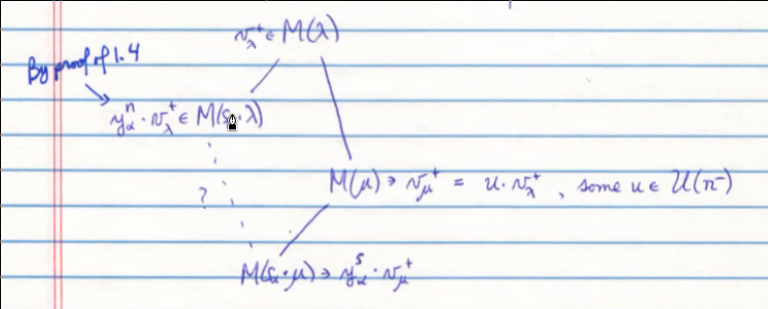
\includegraphics{figures/2020-03-30-09:29.png}\\

Apply the lemma about nilpotent lie algebras to
\(\lien^-, y_\alpha, u\), and \(n\), then there exists a \(t>0\) such
that \(y_\alpha^t u \in U(\lien^-) y_\alpha^n\). Then
\begin{align*}\label{star}
y_\alpha^t \cdot v_\lambda^+ = y_\alpha^t u \cdot v_\lambda^+ \in U(\lien^-) y_\alpha^n \cdot v_\lambda^+ \subseteq M(s_\alpha \cdot \lambda)
.\end{align*}

Now there are two cases.

\textbf{Case 1}:

If \(t\leq s\), we can apply \(y_\alpha^{s-t}\) to equation star to
obtain \(y_\alpha^s \cdot v_\lambda^+ \in M(s_\alpha \cdot \lambda)\).
Thus we have the containment we wanted to prove.

\textbf{Case 2}:

Suppose \(t > s\). We can't divide in the enveloping algebra, but recall
the identity in lemma 1.4(c): \begin{align*}
[x_\alpha y_\alpha^t] = t y_\alpha^{t-1} \qty{ h_\alpha - t + 1}
.\end{align*}

Thus \begin{align*}
[x_\alpha y_\alpha^t] \cdot v_\mu^+ = t(s-t) y_\alpha^{t-1} \cdot v_\mu^+
.\end{align*}

Calculating the bracket another way, the LHS is equal to
\(x_\alpha y_\alpha^t \cdot v_\mu^+ - y_\alpha^t x_\alpha \cdot v_\mu^+\)
and the second term is zero, so this is in \(M(s_\alpha \cdot \lambda)\)
by equation star. We can then iterate if \(t-1 > s\), reducing the power
of \(y_\alpha\) until we get down to
\(y_\alpha^s \cdot v_\mu^+ \in M(s_\alpha \cdot \lambda)\), in which
case we are done by case 1.

\(\qed\)

\hypertarget{existence-of-embeddings}{%
\subsection{4.6: Existence of
Embeddings}\label{existence-of-embeddings}}

\begin{description}
\tightlist
\item[Theorem (Verma's Thesis: Existence of Embeddings)]
Let \(\lambda \in \lieh\dual\) and \(\alpha\in\Phi^+\) and assume
\(\mu \definedas s_\alpha \cdot \lambda \leq \lambda\). Then
\(M(\mu) \subset M(\lambda)\).
\end{description}

\hypertarget{proof}{%
\subsubsection{Proof}\label{proof}}

Assume \(\lambda \in \Lambda\) is integral and \(\mu\) is linked to
\(\lambda\), all weights involved are integral. Without loss of
generality, \(\mu < \lambda\), since we can apply a Weyl group element
to place it in the dominant Weyl chamber.

\begin{enumerate}
\def\labelenumi{\arabic{enumi}.}
\item
  Since \(\mu\) is integral, choose \(w\in W\) such that
  \(\mu' \definedas w\inv \cdot \mu \in \Lambda^+ - \rho\). Following
  the notation in proposition 4.3, write
  \(w = s_n \cdots s_1, \mu_k = s_k \cdots s_1 \cdot \mu'\). Then
  \(\mu' = \mu_0 \geq \mu_1 \geq \cdots \geq \mu_n = \mu\), which yields
  a chain of inclusions of Verma modules
  \(M(\mu_0) \supset M(\mu_1) \supset \cdots\).
\item
  Set \(\lambda' = w\inv \lambda\) and
  \(\lambda_k = s_k \cdots s_1 \cdot \lambda'\) so
  \(\lambda_0 = \lambda'\) and \(\lambda_n = \lambda\). Note that since
  \(\mu \neq \lambda\), we have \(\mu_k \neq \lambda_k\).
\item
  How are \(\mu_k\) and \(\lambda_k\) related? Set
  \(w_k = s_n \cdots s_{k+1}\). It can be checked that
  \(\mu_k = w_k\inv s_\alpha w_k \cdot \lambda_k = s_{\beta_k} \lambda_k\)
  where \(\beta_k = \abs{w_k\inv} \in \Phi^+\) is the choice of
  whichever is positive by Humphreys 1, Lemma 9.2. In particular,
  \(\mu_k - \lambda_k \in \ZZ \beta_k\).
\item
  We have
  \(\mu' = \mu_0 \geq \cdots \geq \mu_k \geq \mu_{k+1} \geq \cdots \geq \mu_n = \mu\).
  Since \(\lambda'<\mu'\) (because \(\mu'\) is the unique dominant
  weight in \(W\cdot \lambda\) but \(\mu < \lambda\), so the
  inequalities must switch at some \(k\). So say \(\lambda_k < \mu_k\)
  but \(\lambda_{k+1} > \mu_{k+1}\), where \(k\) is chosen to be the
  smallest index for which this happens. Note that all of the weights
  are linked to \(\lambda\).
\item
  We want to show that
  \(M(\mu_{k+1}) \subset M(\lambda_{k+1}), \cdots, M(\mu) = M(\mu_n) \subset M(\lambda_n) = M(\lambda)\).
\item
  First,
  \(\mu_{k+1} - \lambda_{k+1} = s_{k+1} \cdot \mu_k - s_{k+1} \cdot \lambda_k\),
  where the LHS is some negative times \(\beta_{k+1}\), and the RHS is
  equal to \(s_{k+1} \qty{ \mu_k - \lambda_k }\), which is a positive
  times \(\beta_k\) by exercise 1.8. Since \(s_{k+1}\) permutes the
  positive roots other than \(\alpha_{k+1}\), this forces
  \(\beta_k = \beta_{k+1} = \alpha_{k+1}\). So we have
  \(\mu_{k+1} = s_{\alpha_{k+1}} \lambda_{k+1}\) which by proposition
  1.4 implies that \(M(\mu_{k+1}) \subset M(\lambda_{k+1})\).
\item
  Combining 1 and 6, we have
  \(M(\mu_{k+2}) = M(s_{k+2} \cdot \mu_{k+1}) \subset M(\mu_{k+1}) \subset M(\lambda_{k+1})\).
  This is the setup of proposition 4.5 and wither alternative leads to
  \(M(\mu_{k+2}) \subset M(\lambda_{k+2}) = M(s_{\alpha_{k+2}} \cdot \lambda_{k+1})\),
\item
  Since this increases the index, we can iterate step 7 to complete step
  5 and get the desired containment.
\end{enumerate}

\hypertarget{wednesday-april-1st}{%
\section{Wednesday April 1st}\label{wednesday-april-1st}}

\begin{description}
\tightlist
\item[Exercise]
Work through the steps for \(\liesl(3)\), due next Thursday.
\end{description}

Preview of next sections:

\begin{itemize}
\tightlist
\item
  4.8: Simplicity Criterion, General Case

  \begin{itemize}
  \tightlist
  \item
    Now that we know \(M(s_\alpha \cdot \lambda) \subset M(\lambda)\)
    whenever \(s_\alpha \lambda \leq \lambda\) for \(\alpha \in \Phi^+\)
    (and not just \(\alpha \in \Delta\)) we can easily complete the
    proof of theorem 4.4 by copying the argument from the integral case.
  \end{itemize}
\item
  4.9: Blocks of \(\OO\), revisited

  \begin{itemize}
  \tightlist
  \item
    Skip, mainly relevant for nonintegral weights (c.f. Proposition 1.13
    for the description of integral blocks)
  \end{itemize}
\item
  4.10: Example: Antidominant Projectives

  \begin{itemize}
  \tightlist
  \item
    Skip, at least for now
  \end{itemize}
\end{itemize}

\hypertarget{application-to-liesl3-cc}{%
\subsection{\texorpdfstring{4.11: Application to
\(\liesl(3, \CC)\)}{4.11: Application to \textbackslash liesl(3, \textbackslash CC)}}\label{application-to-liesl3-cc}}

The simplest nontrivial case, what can we say about the Verma modules?

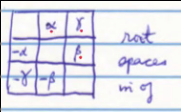
\includegraphics{figures/2020-04-01-09:29.png}\\

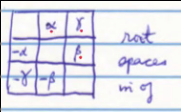
\includegraphics{figures/2020-04-01-09:29.png}\\

We have \(\Delta = \theset{\alpha, \beta}\) and
\(\Phi^+ = \theset{\alpha, \beta, \gamma\definedas \alpha+\beta}\). The
Weyl group is
\begin{align*}
W = \theset{1, s_\alpha,s_\beta, s_\alpha s_\beta, s_\beta s_\alpha, w_0\definedas s_\alpha s_\beta s_\alpha = s_\beta s_\alpha s_\beta  }
.\end{align*}

We first consider an integral regular linkage class \(W\cdot \lambda\),
and we way choose an antidominant \(\lambda\) and assume
\begin{align*}
(\lambda + \rho, \alpha\dual) \in \ZZ^{< 0} \quad \forall \alpha \in \Phi^+ \quad \text{e.g. } \lambda = - 2\rho
\end{align*}

Then \(W_\lambda = \theset{1}\), given by the stabilizer of the isotropy
subgroup, and \(\abs{W\cdot \lambda} = 6\). So there are 6 Verma modules
to understand, and we have the following diamond:

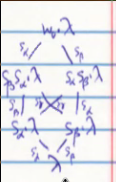
\includegraphics{figures/2020-04-01-09:33.png}\\

The middle two edges are \(s_\gamma\), and each edge corresponds to an
inclusion of Verma modules (with the inclusions going upward). By
Verma's theorem, the Bruhat order corresponds to these inclusions.

\begin{enumerate}
\def\labelenumi{\arabic{enumi}.}
\item
  \(M(\lambda) = L(\lambda)\) since \(\lambda\) is antidominant by
  Theorem 4.4
\item
  By the same theorem, no other \(M(w\cdot \lambda)\) is simple. Then by
  Proposition 4.18, Theorem 4.2c, we have
  \(\soc M(w\cdot \lambda) = L(\lambda)\) for all \(w\in W\)
\item
  Consider \(M(s_\alpha \cdot \lambda)\) and set
  \(\mu \definedas s_\alpha \cdot \lambda\) and the only possible
  composition factors are \(L(\mu)\) and \(L(\lambda)\) and
  \([M(\mu): L(\mu) ] = 1\). If we use Theorem 4.10, this multiplicity
  is 1 in the socle and we're done. If we don't, could it be larger than
  1? Since \(\ext_\OO (L(\lambda), L(\lambda)) = 0\), we can not have
  the following situation:

  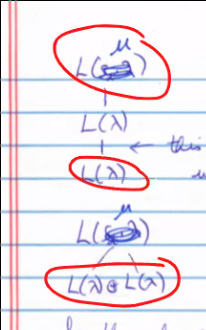
\includegraphics{figures/2020-04-01-09:36.png}\\

  The first extension doesn't exist, since the higher \(L(\lambda)\)
  would drop down to give the bottom diagram, which contradicts
  \(\soc M(\mu) = L(\lambda)\).

  So the only possibilities are multiplicity 1, and
  \(M(s_\alpha \cdot \lambda) = L(s_\alpha \cdot \lambda)\) which lives
  over \(L(\lambda)\), so
  \(\ch L(s_\alpha \cdot \lambda) = \ch M(s_\alpha \cdot \lambda) - \ch M(\lambda)\).

  Similary for \(M(s_\beta \cdot \lambda)\).
\item
  For the higher weights in the orbit, we need more theory. We know
  there are inclusions
  \(x\leq w \implies M(x\cdot \lambda) \subset M(w\cdot \lambda)\)
  according to the Bruhat order - so every edge in the weight poset is a
  reflection, so use Verma's theorem. \begin{align*}
   [M(w\cdot \lambda): L(x \cdot \lambda)] = \begin{cases}
   \geq 1 & ? \\
   0? & ?
   \end{cases}
   .\end{align*}
\end{enumerate}

We'll skip 4.12,4.13, 4.14.

\hypertarget{chapter-5-highest-weight-modules-ii}{%
\subsection{Chapter 5: Highest Weight Modules
II}\label{chapter-5-highest-weight-modules-ii}}

Development by BGG after 1970s, based on partly incorrect proof in
Verma's thesis.

\hypertarget{the-bgg-theorem}{%
\subsubsection{5.1: The BGG Theorem}\label{the-bgg-theorem}}

Which simple modules occur as composition factors of \(M(\lambda)\)?

\begin{description}
\item[Definition (Strongly Linked Weights)]
For \(\mu, \lambda \in \lieh\dual\), write \(\mu \uparrow \lambda\) if
\(\mu = \lambda\) or there exists an \(\alpha \in \Phi^+\) such that
\(\mu = s_\alpha \cdot \lambda < \lambda\),
i.e.~\((\lambda + \rho, \alpha\dual) \in \ZZ^{> 0}\). Extend this
relation transitively: if there exists
\(\alpha_1, \cdots, \alpha_r \in \Phi^+\) such that
\(\mu = (s_{\alpha_1} \cdots s_{\alpha_r}) \cdot \lambda \uparrow (s_{\alpha_2} \cdots s_{\alpha_r} \uparrow \cdots \uparrow s_{\alpha_r} \lambda \uparrow \lambda\),
we again write \(\mu \uparrow\lambda\) and say \(\mu\) is \emph{strongly
linked} to \(\lambda\), yielding a partial order on \(\lieh\dual\).
\item[Theorem (Strong Linkage implies Verma Embedding)]
Let \(\mu, \lambda \in \lieh\dual\).

\begin{itemize}
\tightlist
\item
  (Verma) If \(\mu\uparrow \lambda\) then
  \(M(\mu) \injects M(\lambda)\). In particular,
  \([M(\lambda): L(\mu)] > 0\).
\item
  ??? ???
\end{itemize}
\item[Corollary]
\([M(\lambda): L(\mu)] \neq 0 \iff M(\mu) \injects M(\lambda)\).
\end{description}

The situation is not as straightforward as it might appear (and as Verma
believed). Namely, if
\(0 = M_0 \subset \cdots \subset M_n = M(\lambda)\) is a composition
series and if \(M_i / M_{i-1} \cong L(\mu) \ni \bar v_{\mu}^+\), there
need not be any preimage of \(v_\mu^+\) which is a maximal vector in
\(M(\lambda)\), leading to a map \(M(\mu) \injects M(\lambda)\).

However, when this happens, there will always be some other
\(M_j/M_{j-1} \cong L(\mu)\) where a preimage of a maximal vector
\textbf{is} maximal in \(M(\lambda)\), leading to the required
embedding.

\hypertarget{bruhat-ordering}{%
\subsubsection{5.2 Bruhat Ordering}\label{bruhat-ordering}}

In the case of ``\(\rho\dash\)regular'' integral weights, the BGG
theorem has a nice reformulation in terms of \(W\) and the Bruhat
ordering. Fix \(\lambda \in \Lambda\) antidominant and
\(\rho\dash\)regular, so \((\lambda + \rho, \alpha\dual) \in \ZZ^{< 0}\)
for all \(\alpha\in \Phi^+\).

As in the discussion of \(\liesl(3)\), this means that
\(\abs{W\cdot \lambda} = \abs{W}\) and
\([M(w\cdot \lambda) : L(\mu)] \neq 0\) implying that
\(\mu = x\cdot \lambda\) for some \(x\in W\). What can we say about the
relative positions of \(w\) and \(x\)?

Suppose that \(w\in W, \alpha\in\Phi^+\) and
\(s_\alpha \cdot (w\cdot \lambda) < w\cdot \lambda\) so that
\(M(s_\alpha w \cdot \lambda) \injects M(w\cdot \lambda)\). Our
assumption is equivalent to \begin{align*}
\ZZ^{>0} \ni (w\cdot \lambda + \rho, \alpha\dual) 
&= (w(\lambda+\rho), \alpha\dual)\\
&= (\lambda + \rho, w\inv \alpha\dual) \\
&= (\lambda + \rho, (w\inv\alpha)\dual) \\
&\iff w\inv \alpha \in \Phi^- \iff (w\inv s_\alpha) \alpha \in \Phi^+ \\
&\iff \ell(w) > \ell(w') \quad \text{where } w' = s_\alpha w \\
&\iff w' \mapsvia{s_\alpha} w
.\end{align*}

\hypertarget{friday-april-3rd}{%
\section{Friday April 3rd}\label{friday-april-3rd}}

Recall from last time that we defined a new partial order for all
positive roots generated by ``reflecting down'', namely \emph{strong
linkage}. We had a theorem: \(\mu \uparrow \lambda \implies M(\mu)\)
occurs as a composition factor of \(M(\lambda)\). We also have a
side-arrow notation \(w' \mapsvia{s_\alpha} w\) indicates that
\(w' = s_\alpha w\) and \(w'\) is shorter than \(w\). We conclude that
\(x\cdot \lambda \uparrow w\cdot \lambda \iff x\leq w\) for
\(x, w\in W\), where the RHS is the usual Bruhat order and is notably
independent of \(\lambda\).

\begin{description}
\tightlist
\item[Corollary]
Let \(\lambda \in \Lambda\) be antidominant and \(\rho\dash\)regular and
\(x, w\in W\). Then
\begin{align*}
[M(w\cdot \lambda) : L(x\cdot \lambda)] \neq 0 \iff M(x\cdot \lambda) \injects M(w\cdot \lambda) \iff x \leq w
\end{align*} Note that this statement is why we use antidominant instead
of dominant, since this equation now goes in the right direction.
\end{description}

\hypertarget{jantzen-filtration}{%
\subsection{Jantzen Filtration}\label{jantzen-filtration}}

\begin{description}
\item[Theorem (The Jantzen Filtration and Sum Formula)]
Given \(\lambda \in \lieh\dual\), \(M(\lambda)\) has a terminating
descending filtration satisfying

\begin{enumerate}
\def\labelenumi{\alph{enumi}.}
\item
  Each nonzero quotient has a certain nondegenerate contravariant form
  (3.14)
\item
  \(M(\lambda)^i = N(\lambda)\)
\item

  \begin{align*}\sum_{i > 0} \ch M(\lambda)^i = \sum_{\alpha > 0, s_\alpha \cdot \lambda < \lambda} \ch M(s_\alpha \cdot \lambda)\end{align*}
  (the Integer sum formula, very important)
\end{enumerate}
\end{description}

Note that the sum on the RHS is over
\(\theset{ \alpha\in\Phi^+_{[\lambda]} \suchthat s_\alpha \cdot \lambda < \lambda } \definedas \Phi^+_\lambda\).

\begin{description}
\tightlist
\item[Fact]
\(\soc M(\lambda) = L(\mu)\) for the unique antidominant \(\mu\) in
\(W_{[\lambda]}\cdot \lambda\). Moreover, \([M(\lambda) : L(\mu)] = 1\).
\end{description}

Now suppose \(M(\lambda)^n \neq 0\) but \(M(\lambda)^{n+1} = 0\). Each
\(M(\lambda)^i \supset \soc M(\lambda) = L(\mu)\), since they're
submodules, and each \(M(s_\alpha \cdot \lambda) \supset L(\mu)\), using
the uniqueness of \(\mu\). By looking at coefficients of \(\ch L(\mu)\)
on each side of the sum formula, we obtain \(n = \abs{\Phi^+}\).

\begin{description}
\tightlist
\item[Exercise (5.3)]
When \(\lambda\) is antidominant, integral, and \(\rho\dash\)regular,
then \(n = \ell(w)\). More generally, for nonintegral,
\(n = \ell_\lambda(w)\) where \(\ell_\lambda\) is the length function of
the system \((W_{[\lambda]}, \Delta_{[\lambda]})\).
\end{description}

Some natural questions:

\begin{enumerate}
\def\labelenumi{\arabic{enumi}.}
\tightlist
\item
  Is the Jantzen filtration unique for properties (a)-(c)?
\item
  What are the ``layer multiplicities'' \([M(\lambda): L(\mu)]\)?
\item
  Are the layers \(M(\lambda)\) semisimple? If so, is the Jantzen
  filtration the same as the canonical filtrations with semisimple
  quotients (the radical or socle filtrations)?
\item
  When \(M(\mu) \subset M(\lambda)\), how do the respective Jantzen
  filtrations compare?
\end{enumerate}

A guess for (4): Assume \(\mu \up \lambda\), set
\(r = \abs{\Phi^+_\lambda} - \abs{\Phi_\mu^+}\), which is the difference
in lengths of the two Jantzen filtrations.

Is it true that:

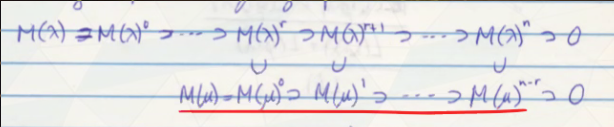
\includegraphics{figures/2020-04-03-09:28.png}\\

with \(M(\mu) \intersect M(\lambda)^i = M(\mu)^{i-r}\) for \(i\geq r\)?

This is called the \emph{Jantzen conjecture} and turns out to be true.

\begin{quote}
Thought equivalent to KL-conjecture, but turned out to be deeper. See
decomposition theorem, sheaves on flag varieties, no simple algebraic
proof until recently. See chapter 8.
\end{quote}

Recall that we obtained a hexagon:

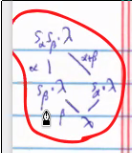
\includegraphics{figures/2020-04-03-09:32.png}\\

We have \begin{align*}
\Phi_{w\cdot \lambda}^{+}=\left\{\gamma \in \Phi^{+} | s_{\gamma} \cdot(w\cdot \lambda)<w \cdot \lambda\right\}=\{\alpha, \alpha+\beta\}
\end{align*}

with corresponding weights
\(s_\gamma(w\cdot \lambda) = s_\beta \cdot \lambda, s_\alpha \cdot \lambda\).
Thus we have a two-step filtration, and we've worked out the characters
of the pieces previously.

Thus \begin{align*}
\sum_{i=1}^n \ch M(w\cdot \lambda)^i 
&= \ch M(s_\alpha \cdot \lambda) + \ch M(s_\beta \cdot \lambda) \\
&= \ch L(s_\alpha \cdot \lambda) + \ch L(s_\beta \cdot \lambda) + 2\ch L(\lambda)
\end{align*}

where we know the last expression explicitly. Since \(n\) has the be the
number of \(L(\lambda)\)s occurring on the RHS, we must have \(n=2\).

We can reason that \(M(w\cdot \lambda)^2 = L(\lambda)\), since any
composition factor in \(M(w\cdot \lambda)^2\) recurs in
\(M(w\cdot \lambda)^1\), and so \begin{align*}
\ch M(w\cdot \lambda)^1 
&= \ch N(w\cdot \lambda) \\
&= \ch L(s_\alpha \cdot \lambda) + \ch L(s_\beta \cdot \lambda) + \ch L(\lambda)
.\end{align*}

We then obtain the following structure on the sections/subquotients of
the Jantzen filtration

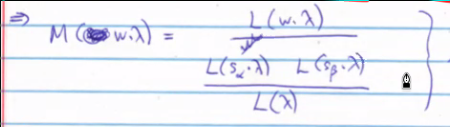
\includegraphics{figures/2020-04-03-09:39.png}\\

where the subquotients move upward through the diagram, e.g.~the middle
is \(M(w\cdot \lambda)^1 / M(w\cdot \lambda)^2\).

\begin{description}
\item[Exercise (Last Assignment)]
\hfill

\begin{enumerate}
\def\labelenumi{\arabic{enumi}.}
\tightlist
\item
  Try to work on the Jantzen filtration sections for
  \(M(w_0 \cdot \lambda)\). List completely any additional assumptions
  or facts needed to deduce \(M(w_0 \cdot \lambda)^i\) uniquely.
\item
  Continue 4.11 in the case where \(\lambda\) is singular Does this
  allow you to deduce that structure of all \(M(w\cdot \lambda)\) using
  the Jantzen sum formula?
\item
  Work out the non-integral case for \(\liesl(3, \CC)\). (There are four
  different cases to consider here.)
\end{enumerate}
\end{description}

\hypertarget{showing-jantzen-implies-bgg}{%
\subsection{Showing Jantzen Implies
BGG}\label{showing-jantzen-implies-bgg}}

We'll prove that
\([M(\lambda) : L(\mu)] \neq 0 \implies \mu \up \lambda\).

\begin{description}
\item[Proof]
By induction on the number of linked weights \(\mu \leq \lambda\)

If \(\lambda\) is minimal in its linkage class, then
\(M(\lambda) = L(\lambda)\) so \(\mu = \lambda\) and
\(\lambda \up \lambda\) trivially.

Otherwise, inductively suppose \([M(\lambda): L(\mu)] > 0\) with
\(\mu < \lambda\). Then \([M(\lambda)^1: L(\mu)] > 0\) since
\(M(\lambda)^1 = N(\lambda)\). By the sum formula,
\([M(s_\alpha \cdot \lambda) : L(\mu)] > 0\) for some
\(\alpha \in \Phi_\lambda^+\). Then \(s_\alpha \cdot \lambda < \lambda\)
so the number of linked weights \(\nu \leq s_\alpha \cdot \lambda\) is
\emph{smaller} than for \(\lambda\).

So by induction,

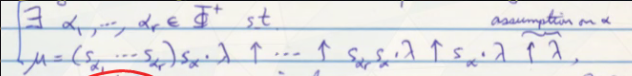
\includegraphics{figures/2020-04-03-09:47.png}\\

and \(\mu \up \lambda\) as required.
\end{description}

Example: \(\liesl(4, \CC)\) with Dynkin diagram
\(\cdot \to \cdot \to \cdot\).

If \(\lambda = (0, -1, 0) \in \Lambda^+ - \rho\) with coordinates with
respect to the fundamental weight basis for \(\Lambda\) or
\(\lieh\dual\). Then take \(w = s_2 s_3, x= s_3 s_2 s_3 s_1 s_2\), then
\(\mu = w\cdot \lambda = (1, -2, -1)\) and
\(\mu - x\cdot \mu = \alpha_1 + \alpha_3\) so \(x\cdot \mu < \mu\).

However, Verma's direct calculations in \(U(\liesl(4, \CC))\) showed
that \(M(x\cdot \mu) \not\subset M(\mu)\), so
\(x\cdot \mu \not\up \mu\).

The explanation (due to Verma) is that \(x\cdot \mu = xw\cdot \lambda\),
using the fact that \(s_1, s_3\) commute, \begin{align*}
xw &= (s_3 s_2 s_3 s_1 s_2) s_2 s_3 \\
&= s_3 s_2 s_3 s_3 s_1 \\
&= s_3 s_2 s_1
.\end{align*}

and \(s_2 s_3, s_3 s_2 s_1\) are not related in the Bruhat order.

\begin{quote}
This is because there is no root reflection relating the two. Note that
this can be seen by considering subexpressions: \(a < b\) iff \(a\)
occurs as some deleted subexpression of \(b\).
\end{quote}

So it's possible to have one weight less than another with no inclusion
of the Verma modules.

\hypertarget{monday-april-6th}{%
\section{Monday April 6th}\label{monday-april-6th}}

Note that most of the theory thus far has not relied on the properties
of \(\CC\), so Jantzen's strategy was to extend the base field to
\(K = \CC(T)\), rational functions in \(T\), then setting
\(g_K \definedas K \tensor_\CC \lieg\). The theory over \(K\) adapts to
\(A = \CC[T]\), the PID of polynomials in one variable \(T\) with \(K\)
as its fraction field and the ``Lie algebra''
\(g_A = A \tensor_\CC \lieg\).

Setup: Let \(A\) be any PID, for example \(\ZZ\) or \(\CC[T]\), and
\(M\) a free \(A\dash\)module of finite rank \(r\). Let \(e, f\in M\)
and suppose \(M\) has an \(A\dash\)valued symmetric bilinear form
denoted \((\wait, \wait)\). Since \(M\) is finite rank, we can choose a
basis \(\theset{e_i}^r\), so the matrix \(F\) of this form relative to
this basis has nonzero determinant \(D\) depending on the choice of
basis. A change of basis is realized by some \(P \in \Gl(r, A)\), giving
\(F' = P^t F P\) (note that forms change by a transpose instead of an
inverse) and \(\det P \in A\units\). Thus \(D\) only changes by a unit
\(u = \qty{\det P}^2\).

We can define the dual module \(M^* = \hom_A(M, A)\) which is also free
of rank \(r\), and contains a submodule \(M\dual\) consisting of
functions \(e\dual: M \to A\) given by \(e\dual(f) = (e, f)\) for any
fixed \(e\in M\). Surprisingly, this doesn't give every hom: e.g.~if the
form only has even outputs. Since \((\wait, \wait)\) is nondegenerate,
the map \(\phi: M\to M\dual\) sending \(e\) to \(e\dual\) is an
isomorphism.

We'll now invoke the structure theory of modules over a PID: There
exists a basis of \(M^*\) given by \(\theset{e+i^*}^r\) where \(M\dual\)
has a basis \(\theset{d_i e_i^*}^r\) for some scalars
\(0\neq d_i \in A\). We can define a dual basis of \(M\) given by
\(\theset{e_i}^r\) where \(e_i^*(e_j) = \delta_{ij}\). We can similarly
get a separate dual basis \(\theset{f_i}\) where
\(f_i\dual = d_i e_i^*\).

We can compare these two bases:
\begin{align*}
(e_i, f_j) = f_j\dual(e_i) = d_j e_j^* (e_i) = d_j \delta_{ij}
\end{align*} (Formula 1)

Thus up to units, \(D = \prod_{i=1}^r d_i\), so this hybrid matrix is
one way to compute this determinant.

Fix a prime element in \(A\), then there is an associated valuation
\(v_p: A \to \ZZ^+\) where \(v_p(a) = n\) if \(p^n \divides a\) but
\(p^{n+1}\notdivides a\). Since \(p\) is prime,
\(\bar M \definedas M/pM\) makes sense and is a finitely generated
module over the field \(\bar A = A/pA\); thus \(\bar M\) is a vector
space.

We'll now define a filtration: for \(n\in \ZZ^+\), define
\(M(n) = \theset{e\in M\suchthat (e, M) \subset p^n A}\). Then
\begin{align*}
M = M(0) \supset M(1) \supset \cdots
\end{align*} is a decreasing filtration, with corresponding images
\(\bar{M(n)}\) that are vector spaces.

\begin{description}
\item[Lemma]
For \(A\) a PID, \(p\in A\) prime, \(\bar A = A/pA\) with valuation
\(v_p\) and \(M\) a free \(A\dash\)module with a nondegenerate symmetric
bilinear form wrt some basis of \(M\) having nonzero determinant \(D\)
Then

\begin{enumerate}
\def\labelenumi{\alph{enumi}.}
\tightlist
\item
  \(v_p(D) = \sum_{n > 0} \dim_{\bar A} \bar{M(n)}\).
\item
  For each \(n\), the modified bilinear form
  \((e, f)_n \definedas p^{-n} (e, f)\) on \(M(n)\) induces a
  nondegenerate form on \(\bar{M(n)} / \bar{M(n+1)}\).
\end{enumerate}
\item[Proof (of (a))]
\hfill

\begin{enumerate}
\def\labelenumi{\arabic{enumi}.}
\tightlist
\item
  For \(f\in M\), write \(f = \sum a_ij f_j\) in terms of the given
  basis, and \((e_i, f) = a_i d_i\). For \(n> 0\), we have

  \begin{center}
    \begin{align*}
    f \in M(n) & \iff v_p((e_i, f)) \geq n \forall i \\
    & \iff v_p(a_i d_i) \geq n \\
    & \iff v_p(a_i) + v_p(d_i) \geq n \\
    & \iff v_p(a_i) \geq n - n_i \quad n_i \definedas v_p(d_i)
    \end{align*}
    \end{center}
\end{enumerate}

This \(a_i\) must be divisibly by \(p\) at least \(n-n_i\) times. This
\(M(n)\) is spanned by
\(\theset{f_i \suchthat n_i \geq n} \union \theset{p^{n-n_i}f_i \suchthat n_i < n}\).

\begin{enumerate}
\def\labelenumi{\arabic{enumi}.}
\setcounter{enumi}{1}
\tightlist
\item
  So \(\bar{M(n)}\) has basis \(\theset{\bar f_i \suchthat n_i \geq n}\)
  and \(\dim \bar{M(n)} = \# \theset{i \suchthat n_i \geq n}\). In
  particular, \(\bar{M(n)} = 0\) for \(n\gg 0\) since there are only
  finitely many \(n_i\). Thus
\end{enumerate}

\begin{center}
  \begin{align*}
  \sum_{n > 0} \dim \bar{M(n)}
  &= \sum_{n > 0} \# \theset{i \suchthat n_i > n} \\
  &= \sum_{i=1}^r n_i \\
  &= \sum_{i=1}^r v_p (d_i) \\
  &= v_p \qty{ \prod_{i=1}^r d_i } \\
  &= v_p(D)
  \end{align*}
  \end{center}
\item[Proof ( of (b) )]
\hfill

\begin{enumerate}
\def\labelenumi{\arabic{enumi}.}
\tightlist
\item
  Note that \((e, f) \in p^n A \implies (e, f)_n \in A\), so this is
  well-defined on \(M(n)\). To see that it's well-defined on
  \(\bar{M(n)}\) we must show that \(e \in p M(n)\).
  \begin{align*}
    (e, pM(n))_n \subset pA \\
    \implies (e, M(n))_n \subset p^{-n}(pM, M(n)) \subset p^{-n+1}(M, M(n)) \subset p^{-n+1}p^n A = pA
    \end{align*} So there is an induced form \((\bar e, \bar f)_n\) on
  \(\bar{M(n)}\).
\end{enumerate}

To show it's nondegenerate, need to compute the radical.

\begin{itemize}
\item
  If \(f\in M(n+1)\) then
  \begin{align*}
  (f, M(n))_{n}=p^{-n}(f, M(n)) \in p^{-n}(f, M) e p^{-n} p^{n+1} A=p A
  \end{align*}

  so \(\bar f \in \rad (\wait, \wait)_n\)
\item
  See notes.
\end{itemize}
\end{description}

\hypertarget{wednesday-april-8th}{%
\section{Wednesday April 8th}\label{wednesday-april-8th}}

Recall that we are setting up Jantzen's filtration. Let \(A\) be a PID,
\(\mfp \in A\) prime, \(\bar A = A/pA\), \(M\) a free \(A\dash\)module
of rank \(r\), with a nondegenerate symmetric bilinear form
\((\wait ,\wait)\) having nonzero determinant wrt some basis of \(M\).
Define \(M(n), \bar{M(n)}\) as before

\begin{description}
\item[Lemma]
\hfill

\begin{enumerate}
\def\labelenumi{\arabic{enumi}.}
\tightlist
\item
  \(v_p(D) = \sum_{n > 0} \dim_{\bar A} \bar{M(n)}\)
\item
  For each \(n\), the modified bilinear form induces a nondegenerate
  form on \(\bar{M(n)} / p\bar{M(n)}\)?
\end{enumerate}
\end{description}

\hypertarget{proof-of-jantzens-theorem}{%
\subsection{Proof of Jantzen's
Theorem}\label{proof-of-jantzens-theorem}}

Let \(A = \CC[T]\) and \(K = \CC(T)\) its fraction field, and let
\(\lieg_A = A \tensor_\CC \lieg\) and \(\lieg_K = K \tensor_\CC \lieg\),
which is a Lie algebra that is split over \(K\), i.e.~every
\(h\in \lieh_K = K \tensor_\CC \lieh\) has all eigenvalues of \(\ad h\)
in \(K\).

The theory we need carries over to the extended setting. The plan is the
following:

\begin{itemize}
\tightlist
\item
  Construct and look at basic properties of Verma modules (1.3-1.4)
\item
  Look at properties of their contravariant forms (3.14 - 3.15)
\item
  Find a simplicity criterion (4.8)
\end{itemize}

We'll use Lemma 5.6 to construct filtrations on the weight spaces of the
extended Verma module, then reduce mod \(T\) (using evaluation
morphisms) to assemble the Jantzen filtration for the original
\(\CC\dash\)module.

Given \(\lambda \in \lieh\dual\), set
\(\lambda_T = \lambda + T_\rho \in \lieh_K\dual\). For all
\(\alpha\in \Phi\), we have \begin{align*}
(\lambda_T  + \rho, \alpha\dual) =
(\lambda + \rho , \alpha\dual) + T(\rho, \alpha\dual) \not\in \ZZ
,\end{align*} since this is a linear polynomial. So \(\lambda_T\) is
antidominant.

Therefore \(M(\lambda_T)\) is simple, and equivalently (unique up to
scalars) its nonzero contravariant form is nondegenerate.

The module \(U(\lieg_A) \cong A \tensor_\CC U(\lieg)\) is a natural
``\(A\dash\)form'' of \(U(\lieg_K) \cong K \tensor_\CC U(\lieg)\). This
yields \(M(\lambda_T)_A\), an \(A\dash\)form of \(M(\lambda_T)\), where
each weight space is an \(A\dash\)module of finite rank.

Some remarks about contravariant forms on highest weight modules: given
\(M\) and such a form \((\wait, \wait): M\cross M \to \CC\), the
transpose serves as an adjoint and we have
\((uv, v') = (v, \tau(u) v')\).

Distinct weight spaces are orthogonal, i.e.~\((M_\mu, M_\nu) = 0\) since
\begin{align*}
(hv, v') = \mu(h) (v, v') \\
= (v, hv') = \nu(h) (v, v') \\
\end{align*} where \(\mu(h) \neq \nu(h)\), implying \((v, v') = 0\).

We can compute \begin{align*}
(u v^+ \in M_\mu, u' v^+ \in M_\mu) = (v^+, \tau(u) u' v') = a (v^+, v^+)
\end{align*}

for some \(a\in A\), since \(\lambda_T = \lambda + T_p\) maps
\(\lieh_A \to A\). We can use the decomposition
\(U(\lieg) = U(\lieh) \oplus (\lien^- U(\lieg) + U(\lieg) \lien)\),
where \(\lien^+\) kills \(v^+\) and \(\lien^-\) lowers into an
orthogonal weight space, and so this pairing only depends on
\((v^+, v^+)\).

\begin{quote}
Note that the radical of this bilinear form is a maximal submodule.
\end{quote}

The weights are of the form \(\lambda_T - \nu\) for
\(\nu \in \lien^+ \Phi^+ = \Lambda_r^+\). Apply lemma 5.6 to the
\(A\dash\)form \(M_{\lambda - \nu}\) of
\(M(\lambda_T)_{\lambda_T - \nu}\) to get a decreasing finite filtration
of \(A\dash\)submodules

\begin{align*}
M_{\lambda-\nu}(0)=M_{\lambda_{T}-v}(1) \supset \cdots
\end{align*}

where
\(M_{\lambda_T - \nu}(i) = \theset{e\in M_{\lambda_T - \nu} \suchthat (e, M_{\lambda_T - \nu}) \subset T^i A}\).

For each \(i \geq 0\), set
\(M(\lambda_T)_A^i = \sum_{\nu \in \Lambda_r^+} M_{\lambda_T - \nu}(i)\).
This yields a decreasing filtration of \(A\dash\)submodules.

Next we want to ``set \(T=0\)'': formally, pass to the quotient
\(\bar M = M/TM\) over the field \(\bar A = A/TA \cong \CC\). Since
\(\lambda_T = \lambda + T_\rho \mapsvia{T = 0} \lambda\), we have
\(M(\lambda_T)_A \cong M(\lambda)\) and the filtration becomes a
decreasing filtration of \(M(\lambda)\).

By the lemma, the sections of this filtration inherit nondegenerate
contravariant forms, proving (a). By the proof of that lemma, the
filtration on each individual weight space terminates at 0.

Claim: Some \(M(\lambda)^{n+1} = 0\).

\begin{description}
\tightlist
\item[Proof]
If not, since \(M(\lambda)\) has finite length, we must have
\(0 \neq M(\lambda)^n = M(\lambda)^{n+1} = \cdots\) for some \(n\).
Choose some \(u\in \lieh\dual\) such that \(M(\lambda)_\mu^n = 0\), but
then \(0 \neq M(\lambda)_\mu^n = M(\lambda)_\mu^n = \cdots\), a
contradiction.
\end{description}

For a proof of (c), we want to show
\(\sum_{i > 0} \ch M(\lambda)^i = \sum_{\alpha \in \Phi^+} \ch M(s_\alpha \cdot \lambda)\).
We can show that the LHS is given by \begin{align*}
\cdots
&= \sum_{i > 0} \sum_{\nu \in \Lambda_r^+} \dim M(\lambda)_{\lambda-\nu}^i \\
&= \sum_{i > 0} \sum_\nu \dim\qty{\bar{M(\Lambda_T)_A^i}}_{\lambda_T - \nu} e(\lambda - v) \\
&= \sum_i \sum_\nu \dim \bar{M_{\lambda_T -\nu}(i)} e(\lambda - \nu) \\
&= \sum_\nu \sum_i \dim \bar{M_{\lambda_T -\nu}(i)} e(\lambda - \nu) \\
&= \sum_\nu v_T(D_\nu(\lambda_T)) e(\lambda - v) \quad\text{Lemma 5.6a}
.\end{align*}

where \(D_\nu(\lambda_T)\) is the determinant of the matrix of the
contravariant form on the \(\lambda_T - \nu\) weight space of
\(M(\lambda_T)\).

Fact (Jantzen, Shapovalov): Up to a nonzero scalar multiple depending on
a choice of basis of \(U(\lien^-)\), \begin{align*}
D_\nu(\lambda_T) = \prod_{\alpha > 0} \prod_{r \in \ZZ^{>0}} \qty{ (\lambda_T, \rho, \alpha\dual) - r  }^{P(\nu - r_\alpha)}
\end{align*} where \(P\) is the Kostant partition function.

We can calculate \(v_T\) of this, which doesn't depend on the scalar:
\begin{align*}
(\lambda_T + \rho, \alpha\dual) - r = (\lambda+\rho, \alpha\dual) -r + T(\rho, \alpha\dual)\\
\implies v_T( \cdots ) =
\begin{cases}
1 & (\lambda + \rho, \alpha\dual) = r > 0 \iff \alpha \in \Phi_\lambda^+ \\
0 & \text{else}
\end{cases}
.\end{align*}

We then have \begin{align*}
v_T(D_\nu(\lambda_T)) = \sum_{\alpha \in \Phi^+_\lambda} P(\nu - (\lambda + \rho, \alpha\dual)\alpha)
.\end{align*}

Thus the LHS is given by \begin{align*}
\cdots
&= \sum _{\nu \in \Lambda_r^+} \sum_{\alpha\in \Phi_\lambda^+} P(\nu - (\lambda + \rho, \alpha\dual) \alpha) e(\lambda - \nu) \\
&= \sum _{\alpha \in \Phi_\lambda^+} \sum_{\sigma \in \Lambda_r^+} P(\sigma) e(\lambda - (\lambda + \rho, \alpha\dual)\alpha - \sigma) \\
&= \sum_{\alpha \in \Phi_\lambda^+} \ch M(s_\alpha \cdot \lambda)
,\end{align*}

where we've used what we know about characters of Verma modules.

\begin{quote}
Note that the proof of the determinant formula is technical.
\end{quote}

We'll skip chapter 6 on KL theory.

\hypertarget{friday-april-10th}{%
\section{Friday April 10th}\label{friday-april-10th}}

\hypertarget{translation-functors}{%
\subsection{Translation Functors}\label{translation-functors}}

Extremely important, allow mapping functorially between blocks
(recalling \(\OO = \bigoplus \OO_{\chi_\lambda}\)) and in good
situations gives an equivalence of categories.

\begin{description}
\tightlist
\item[Definition (Projection Functors)]
A \emph{projection functor}
\(\mathrm{pr}_\lambda: \OO \to \OO_{\chi_\lambda}\) where
\(M = \bigoplus_\mu M^{\chi_\mu} \mapsto M^{\chi_\lambda}\).
\end{description}

Convention: From now on, all weights will be integral

\begin{description}
\item[Proposition (Properties of Projection Functors)]
\hfill

\begin{enumerate}
\def\labelenumi{\arabic{enumi}.}
\tightlist
\item
  \(\mathrm{pr}_\lambda\) is an exact functor.
\item
  \(\hom(M, N) \cong \bigoplus_\lambda \hom(\mathrm{pr}_\lambda M, \mathrm{pr}_\lambda N)\)
\item
  \(\mathrm{pr}_\lambda (M\dual) = (\mathrm{pr}_\lambda M)\dual\)
\item
  \(\mathrm{pr}_\lambda\) maps projectives to projectives
\item
  \(\mathrm{pr}_\lambda\) is self-adjoint
\end{enumerate}
\item[Proof]
\hfill

\begin{enumerate}
\def\labelenumi{\arabic{enumi}.}
\tightlist
\item
  Given
  \begin{align*}0 \mapsvia f N \mapsvia g P \to 0,\end{align*} we can
  decompose this as
  \begin{align*}0 \to \bigoplus_\lambda M^{\chi_\lambda} \mapsvia{\oplus f_\lambda} \bigoplus_\lambda N^{\chi_\lambda} \mapsvia {\oplus g_\lambda} \bigoplus_\lambda P^\lambda \to 0,\end{align*}
  which gives exactness on each factor.
\item
  We can move direct sums out of homs.
\item
  Write
  \(\mathrm{pr}_\lambda \qty{ \qty{\bigoplus M^{\chi_\lambda} }\dual }\)
  and use theorem 3.2b to write as \((M^{\chi_\lambda})\dual\).
\item
  \(\mathrm{pr}_\lambda(P)\) is a direct summand of a projective and
  thus projective.
\item
  We have
  \(\hom(\mathrm{pr}_\lambda M, N) = \hom(\mathrm{pr}_\lambda M, \mathrm{pr}_\lambda N) = \hom(M, \mathrm{pr}_\lambda N)\).
\end{enumerate}
\item[Definition (Translation Functors)]
Let \(\lambda, \mu \in \Lambda\) with \(\nu = \mu - \lambda\) integral.
Then there exists \(w\in W\) such that
\(\tilde \nu \definedas w\nu \in \Lambda^+\) is in the dominant chamber.
Define the \emph{translation functor}
\begin{align*}T_\lambda^\mu = \mathrm{pr}_\mu(L(\tilde \nu) \tensor_\CC \mathrm{pr}_\lambda(M)),\end{align*}
where we use the fact that \(\tilde \nu\) dominant makes
\(L(\tilde \nu)\) finite-dimensional.
\end{description}

This is a functor \(\OO^{\chi_\lambda} \to \OO^{\chi_\mu}\).

\begin{description}
\item[Proposition (Propoerties of Translation Functors)]
\hfill

\begin{enumerate}
\def\labelenumi{\arabic{enumi}.}
\tightlist
\item
  The translation functor is exact.
\item
  \(T_\lambda^\mu (M\dual) = \qty{T_\lambda^\mu M}\dual\)
\item
  It maps projectives to projectives.
\end{enumerate}
\item[Proof]
\hfill

\begin{enumerate}
\def\labelenumi{\arabic{enumi}.}
\tightlist
\item
  It is a composition of exact functors, noting that tensoring over a
  field is always exact.
\item
  Use proposition 12, \(L(\tilde \nu)\) is self-dual, and
  \(A\dual \tensor B\dual \cong (A\tensor B)\dual\).
\item
  Use proposition 1 and previous results, e.g.~\(L \tensor_\CC (\wait)\)
  preserves projectives if \(\dim L < \infty\) (Prop 3.8b).
\end{enumerate}
\item[Proposition (Adjoint Property of Translation Functor)]
\(\hom(T_\lambda^\mu M, N) \cong \hom(M, T_\mu^\lambda N)\), which also
holds for every \(\ext^n\).
\item[Proof]
We have

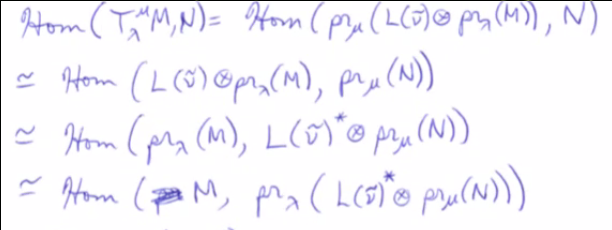
\includegraphics{figures/image_2020-04-10-09-26-51.png}\\

But \(L(\tilde \nu)\dual \cong L(-w_0 \tilde \nu)\) and
\(-w_0 \tilde \nu = w_0 w(\lambda - \mu)\) is the dominant weight in the
orbit of \(\lambda - \mu\) used to define \(T_\mu^\lambda\).

For the second part, use a long exact sequence -- if two functors are
isomorphic, then their right-derived functors are isomorphic.
\end{description}

Does this functor take Vermas to Vermas? I.e. do we have
\(M(w\cdot \lambda) \mapsto M(w\cdot \mu)\) when
\(T_\lambda^\mu \OO_{\chi_\lambda} \to \OO_{\chi_\mu}\)?

Picture for \(\liesl(3, \CC)\):

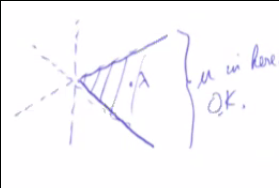
\includegraphics{figures/image_2020-04-10-09-32-13.png}\\

This doesn't always happen, and depends on the geometry.

\hypertarget{weyl-group-geometry-facets}{%
\subsubsection{Weyl Group Geometry --
Facets}\label{weyl-group-geometry-facets}}

\begin{description}
\item[Definition (Facets)]
Given a partition of
\(\Phi^+ = \Phi^0_F \union \phi^+_F \union \Phi^-_F\), a \emph{facet}
associated to this partition is a nonempty set consisting of solutions
\(\lambda \in E\) to the following equations:

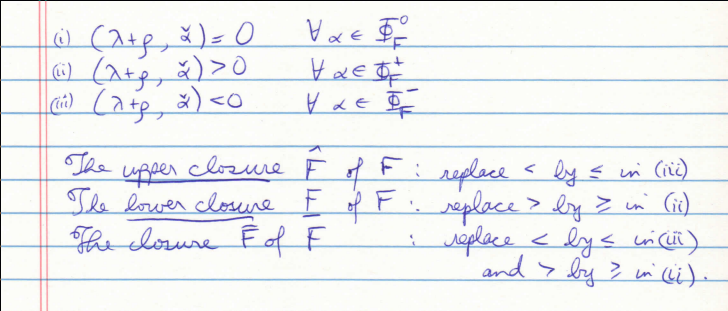
\includegraphics{figures/image_2020-04-10-09-36-18.png}\\
\end{description}

Example: \(A_2\), where
\(\Phi^+ = \theset{\alpha, \beta, \alpha + \beta}\).

\begin{enumerate}
\def\labelenumi{\arabic{enumi}.}
\tightlist
\item
  Take \(\Phi_F^0 = \Phi^+\), and by the orthogonality conditions,
  \(F = \theset{-\rho}\) since it must be orthogonal to all 3 roots. So
  the origin is a facet.
\item
  Take \(\Phi_F^0 \theset{\alpha, \beta}\) and
  \(\Phi_F^+ = \theset{\alpha + \beta}\), so \(F = \emptyset\) can not
  be a facet.
\item
  See notes
\item
  see notes
\end{enumerate}

Note that \(\bar F \supset \hat F \union \underbar F\) in general.

\hypertarget{monday-april-13th}{%
\section{Monday April 13th}\label{monday-april-13th}}

Reviewing the definition of \emph{facets}. We partitioned \(\Phi\) into
3 sets \(\Phi_F^{0, \pm}\), some of which could be empty. We had notion
of upper and lower closure given by replacing the strict inequalities
with inequalities in condition (3) and (2) respectively.

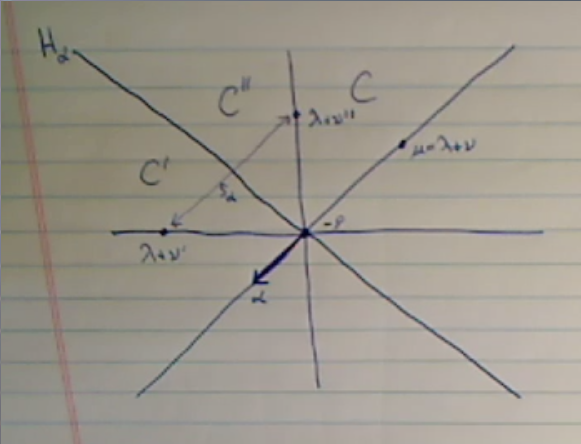
\includegraphics{figures/image_2020-04-13-09-07-07.png}\\

\begin{description}
\tightlist
\item[Definition (Chambers)]
If \(F\) is a facet with \(\Phi_F^0=\emptyset\), then \(F\) is called a
\emph{chamber}.
\end{description}

A facet with exactly 1 root in \(\Phi_F^0\), then this is called a
\emph{wall}.

Observations:

\begin{enumerate}
\def\labelenumi{\arabic{enumi}.}
\tightlist
\item
  \(\Phi^+ = \Phi_F^+\) always defines a chamber called the
  \emph{fundamental chamber} and is denoted \(C_0\).
\item
  If \(F\) is any chamber, then \(F = w\cdot C_0\) for some \(w\in W\).
\end{enumerate}

\begin{description}
\item[Proposition (Relation Between Facets and Chambers)]
\hfill

\begin{enumerate}
\def\labelenumi{\alph{enumi}.}
\tightlist
\item
  Every facet \(F\) is the upper closure of some unique chamber \(C\).
\item
  If \(F \subset \hat C\) then \(\hat F \subset \hat C\).
\end{enumerate}
\item[Proof]
\hfill

\begin{enumerate}
\def\labelenumi{\alph{enumi}.}
\tightlist
\item
  If \(F\) is given by \(\Phi_F^0 \union \Phi_F^+ \union \Phi_F^-\) and
  \(C\) pairs with \(\Phi_C^+ = \Phi_F^+\) and thus
  \(\Phi_C^- = \Phi_F^- \union \Phi_F^0\). To see that
  \(C\neq \emptyset\), use remark (1) on page 132.
\item
  Obvious from above description of \(C\).
\end{enumerate}
\end{description}

\hypertarget{key-lemma-from-7.5}{%
\subsection{Key Lemma from 7.5}\label{key-lemma-from-7.5}}

We're focusing only on integral weights, and we want to calculate the
translation functor of a Verma \(T_\lambda^\mu M(\lambda)\). First step:
project onto \(\lambda\) block, but \(M(\lambda)\) is in that block
already. Then tensor with \(L(\tilde \nu)\), then the product has a
standard filtration with certain Verma section
\(M(\lambda + w\tilde \nu)\), each occurring with multiplicity one. The
weight \(\tilde \nu\) is the unique dominant weight in the orbit of
\(\mu - \lambda\), one of the Verma sections is in \(M(\mu)\). We plan
to show that \(T_\lambda^\mu M(\lambda) = M(\mu)\) in ``good''
situations.

\begin{description}
\item[Lemma]
Let \(\lambda, \mu \in \Lambda\) be integral weights and
\(\nu = \mu - \lambda\) and
\(\tilde \nu \in \Lambda^+ \intersect W \nu\) (which is unique). Assume
there is a facet \(F\) with \(\lambda \in F, \mu \in \bar F\). Then for
all weights \(\nu' \neq \nu\) of \(L(\tilde\nu)\), the weight
\(\lambda + \nu'\) is \emph{not} linked to \(\lambda + \nu = \mu\) under
\(W\).
\item[Proof]
\hfill

Toward a contradiction, suppose there exists \(\nu \neq \nu\) in
\(\Pi(L(\tilde \nu))\) with
\(\lambda + \nu' \in W\cdot (\lambda + \nu)\). Define the
\emph{distance} between two chambers \(C, C'\) as the number of root
hyperplanes separating them. Under the correspondence between chambers
and \(W\) given by picking a fundamental chamber, the distance
corresponds to the difference in lengths between the corresponding Weyl
group elements.

\hfill\break

So choose chambers \(C, C'\) with \(F \subset \bar C\),
\(\lambda + \nu' \in \bar C'\), and \(d(C, C')\) is minimal. We now go
through 14 easy steps.

\hfill\break

\begin{enumerate}
\def\labelenumi{\arabic{enumi}.}
\tightlist
\item
  The case \(d(C, C') = 0\) is impossible, since this would force
  \(C =C'\)/ But \(C\) is a fundamental domain for the dot action, where
  \(C' \ni \lambda + \nu' \neq \lambda + \nu = \mu \in \bar F \subset \bar C\).
  This contradicts \(C\) being a fundamental domain, since each ? will
  be conjugate to a \emph{unique} element.
\item
  The case \(d(C, C') > 0\) implies there's a hall
  \(H_\alpha \intersect \bar C '\) of \(C'\) separating \(C'\) from
  \(C\). Wlog assume \(C'\) is on the positive side of \(H_\alpha\) and
  \(\alpha > 0\) and \(C\) is on the negative side. Since
  \(\bar F \subset \bar C\), we have
  \((\xi + \phi, \alpha\dual) \leq 0\) for all \(\xi \in \bar F\).
\item
  Reflect and set \(C'' \definedas s_\alpha C'\), then
  \(d(C, C'') < d(C, C')\) and we will be able to apply the induction
  hypothesis.
\item
  By (2), \((\lambda + \nu' + \rho, \alpha\dual) \geq 0\) since
  \(\lambda + \nu'\) was on the positive side.
\item
  By (2), \((\lambda + \rho, \alpha\dual) \leq 0\) since
  \(\lambda + \nu'\) was on the negative side.
\item
  By (4),
  \(\lambda + \nu' \geq s_\alpha \cdot (\lambda + \nu') = s_\alpha \cdot \lambda + s_\alpha \nu' = \lambda - (\lambda + \rho, \alpha\dual)\alpha + s_\alpha \nu' \definedas \nu''\)
  by just applying the formula for the dot action.
\item
  By (5) and (6),
  \(s_\alpha \nu' \leq s_\alpha \nu' - (\lambda + \rho, \alpha\dual) \alpha \leq \nu'\),
  where the first and last terms are weights of \(L(\tilde \nu)\), so
  \(\nu'' \leq \nu'\). In fact, this inequality is obtained by
  cancelling \(\lambda\) and adding/substracting multiples of
  \(\alpha\), so these come from an \(\alpha\) root string.
\item
  Rewriting (6), we have
  \(s_\alpha (\lambda + \nu') = \lambda + \nu'' \in s_\alpha \bar {C'} = \bar {C''}\).
\item
  By 1.6 bullet (2) in Humphreys, \(\nu'' \in \Pi (L(\tilde \nu))\).
\item
  By the minimality assumed for \(\nu'\), along with (3), (8), (9), we
  have \(\nu'' = \nu\).
\item
  Rewriting (7) and using the hypothesis \(\nu \neq \nu'\), we can write
  \(s_\alpha \nu ' \leq \nu < \nu'\) where the inequality is strict
  because they are not equal. This is still an \(\alpha\) root string of
  weights in the simple module \(L(\tilde \nu)\) with
  \(\nu \in W\tilde \nu\). The first inequality can \emph{not} be
  strict, otherwise \(v\pm \alpha\) would both be weights of
  \(L(\tilde \nu)\), contradicting Humphreys 1.6 bullet 1. So
  \(s_\alpha \nu' = \nu\).
\item
  By (10), (11), and (6),
  \(s_\alpha \nu' = \nu = \nu'' = s_\alpha \nu ' - (\lambda + \rho, \alpha\dual) \alpha\),
  so \((\lambda + \rho, \alpha\dual) = 0\).
\item
  Since \(\lambda \in F\) by assumption, if \(\alpha \in \Phi_F^0\) then
  \((\xi + \rho, \alpha\dual) = 0\) for all \(\xi \in \bar F\). In
  particular, for \(\xi = \mu = \lambda + \nu\), and combined with (12),
  this say \((\nu, \alpha\dual) = 0\) since the pairing is linear in the
  first slot.
\item
  We're now done: combining (11), (13) yields
  \(\nu ' = s_\alpha \nu = \nu - (\nu, \alpha\dual)\alpha = \nu\), which
  contradicts \(\nu \neq \nu'\).
\end{enumerate}
\end{description}

\hypertarget{translation-functors-and-verma-modules}{%
\subsection{7.6: Translation Functors and Verma
Modules}\label{translation-functors-and-verma-modules}}

\begin{description}
\item[Theorem (Translation Functors on Vermas for Antidominant Weights)]
Let \(\lambda, \mu \in \Lambda\) be antidominant. Assume there is a
facet \(F\) relative to the dot action of \(W\) with \(\lambda \in F\)
and \(\mu \in \bar F\). Then for all \(w\in W\), we have \begin{align*}
T_\lambda^\mu M(w\cdot \lambda) &= M(w\cdot \mu) \\
T_\lambda^\mu M(w\cdot \lambda)\dual &\cong M(w\cdot \mu)\dual
.\end{align*}
\item[Proof]
Apply the previous lemma to \(w\cdot \lambda, w\cdot \mu\) and the facet
\(w\cdot F\) using \(\nu = w\cdot \mu - w\cdot \lambda\). To compute
\(T_\lambda^\mu\), first consider
\(L(\tilde \nu) \tensor M(w\cdot \lambda)\). By Theorem 3.6, this has a
standard filtration with quotients \(M(w\cdot \lambda + \nu')\) for
\(\nu' \in \Pi(L(\tilde \nu))\), potentially with multiplicity.

\hfill\break

In particular, \(M(w\cdot \mu) = M(w\cdot \lambda + \nu)\) appears
exactly once. By the lemma, none of the other highest weights
\(w\cdot \lambda + \nu'\) are linked to \(\mu\). Thus decomposing the
tensor product into direct summands in infinitesimal blocks, the only
summand in \(\OO_{\chi_\mu}\) is \(M(w\cdot \mu)\). Therefore
\(T_\lambda^\mu M(w\cdot \lambda) = \pr_\mu (L(\tilde \nu) \tensor M(w\cdot \lambda)) = M(w\cdot \mu)\).
The statement about duals follows from translation functors commuting
with taking duals.
\end{description}

\hypertarget{wednesday-april-15th}{%
\section{Wednesday April 15th}\label{wednesday-april-15th}}

Section 7.6, proved theorem about translation functors on Verma modules.
We fixed an antidominant weight, since we can apply elements of \(W\) to
obtain the rest. We proved that translation functors take Verma modules
to Verma modules.

\begin{description}
\tightlist
\item[Corollary (Translations Have Standard Filtrations)]
If \(M\in \OO_\chi\) has a standard filtration, then so does
\(T_\lambda^\mu M \in \OO_\mu\).
\item[Proof]
By induction on the length of the filtration, where the length 1 case is
handled by the theorem. In general we have
\(0 \to N \to M \to M(w\cdot \lambda) \to 0\) and since
\(T_\lambda^\mu\) is exact, we can apply it to get another exact
sequence. ??? See notes.
\end{description}

\hypertarget{translation-functors-and-simple-modules}{%
\subsection{Translation Functors and Simple
Modules}\label{translation-functors-and-simple-modules}}

\begin{description}
\tightlist
\item[Proposition (Translation Functors Applied to L for Antidominant
Weights)]
Let \(\lambda, \mu \in \Lambda\) be antidominant with a facet \(F\) such
that \(\lambda \in F\) and \(\mu \in \bar F\). Then for all \(w\in W\),
\(T_\lambda^\mu L(w\cdot \lambda)\) is either \(L(w\cdot \mu)\) or 0.
\end{description}

Idea: we're pushing \(\lambda\) to something more singular.

\begin{description}
\tightlist
\item[Proof]
Apply the exact functor \(T_\lambda^\mu\) to the surjection
\(M(w\cdot \lambda) \surjects L(w\cdot \lambda)\) so obtain
\(M(w\cdot \mu) \surjects M\) for some \(M\). Since \(M\) is a quotient
of a Verma module, it is a highest weight module of highest weight
\(w\cdot \mu\). Suppose \(M\neq 0\), we can apply \(T_\lambda^\mu\) to
\(L(w\cdot \lambda) \injects M(w\cdot \lambda) \dual\) to obtain
\(M(w\cdot \mu) \surjects M \injects M(w\cdot \mu) \dual\), a nonzero
map. By Theorem 3.3c, the image is the socle, so we obtain
\(M \cong L(w\cdot \mu)\).
\end{description}

It turns out that \(T_\lambda^\mu \cong L(w\cdot \mu)\) precisely when
\(w\cdot \mu \in \hat{w\cdot F}\) (the upper closure, see Theorem 7.9
and example 7.7 for \(\liesl(2, \CC)\)). Example: take \(\rho = -1\).

So if we can figure out \(L(w\cdot \lambda)\) for \(\lambda\)
\(\rho\dash\)regular, we can determine the composition factors of all
Verma modules by ``pushing to walls''. There's also a need to ``cross
walls'', and there's a nice rule for what happens for Verma modules in
this case. Going ``off the wall'' on the other side is more complicated.

\hypertarget{category-equivalences}{%
\subsection{7.8: Category Equivalences}\label{category-equivalences}}

We saw in the case of \(\liesl(2, \CC)\) and \(\liesl(3, \CC)\) that the
composition factors depended more on the Weyl group than the highest
weight. We want to show that \(T_\lambda^\mu\) gives an equivalence of
categories between \(\OO_\lambda\) and \(\OO_\mu\). when
\(\lambda, \mu\) are antidominant and lie in the same facet. We'll first
show that it induces an isomorphism on the Grothendieck groups.

\begin{description}
\tightlist
\item[Proposition (Isomorphism of Grothendieck Groups for Weights in a
Common Facet)]
Suppose there is a single facet \(F\) containing \(\lambda, \mu\). Then
the obvious map is an isomorphism: \begin{align*}
T_\lambda^\mu: K(\OO_\lambda) &\mapsvia\cong K(\OO_\mu)\\
[M(w\cdot \lambda)] &\mapsto [M(w\cdot \mu)] \\
[L(w\cdot \lambda)] &\mapsto [L(w\cdot \mu)]
.\end{align*}
\item[Proof]
Recall that \(\theset{[M(w\cdot \lambda)] \suchthat w\in W}\) (and/or
replacing by \(L\)) forms \(\ZZ\dash\)basis for \(K(\OO_\lambda)\) and
similarly for \(\mu\). So when \([M]\in K(\OO_\lambda)\) is written was
a \(\ZZ\dash\)linear combination of \([M(w\cdot \lambda)]\), it's clear
that \(T_\mu^\lambda T_\lambda^\mu [M] = [M]\). So these functors are
mutually inverse.\\
By the previous proposition, if we take \(L\) instead, the result is
either the identity or zero. But zero is impossible by what we just
proved, so we must have
\(T_\lambda^\mu [ L(w\cdot \lambda)] = [L(w\cdot \mu)]\) forcing
\(T_\lambda^\mu L(w\cdot \lambda) = L(w\cdot \mu)\).
\end{description}

Since \(K(\OO) \cong \chi_0\), the group of formal characters of modules
in \(\OO\), we in fact get \begin{align*}
[M: L(w\cdot \lambda)] = [T_\lambda^\mu M: L(w\cdot \mu)] \quad \forall M\in \OO
.\end{align*}

Thus the \(\lambda, \mu\) don't matter as much (as long as they're in
the same facet), and the \(w\) is what's important. There is a theorem
(2005) that for any artinian abelian category, and isomorphism of
Grothendieck groups implies an equivalence of categories.

\hypertarget{wednesday-april-22nd}{%
\section{Wednesday April 22nd}\label{wednesday-april-22nd}}

For \(p\in \QQ[x]\), we'll denote \(p[i]\) the \(i\)th coefficient.

For \(M\in \OO\) or any module of finite length, we define its radical
series:
\begin{align*}\rad^0 M = M,\quad \rad^{i+1} M = \rad(\rad^i M)\end{align*}
Note that the layers/subquotients are semisimple.

Dually, \(\soc M\) is the largest semisimple submodule of \(M\), and
iterating this yields the \emph{socle series}. Denote
\begin{align*}\soc_i M \definedas \soc^{i+1} M / \soc^i M\end{align*}
the \(i\)th socle layer. The corresponding layers are the same as in the
radical filtration, just with reversed indexing.

For convenience, set
\begin{align*}Q_{x, w} = P_{w_0 w, w_0 x}(q)\end{align*} the ``inverse''
KL polynomial. Recall that a consequence of the KL conjecture is that
\([M_w] = \sum_{x\leq w} Q_{x, w}(1) [L_x]\)

The following theorem follows from the Jantzen conjecture

\begin{description}
\item[Theorem (Coefficients of Inverse KL Polynomials)]
\hfill

\begin{enumerate}
\def\labelenumi{\alph{enumi}.}
\item

  \begin{align*}Q_{x, w}[i] = [ \rad_{\ell(xw) - 2i} M_w : L_x] = [\soc_{\ell(x) + 2i} M_w: L_x]\end{align*}

  \begin{quote}
  Note that Humphreys adds \(+1\) here due to indexing.
  \end{quote}
\item
  If \(x < w\), then \(\dim \ext^1 (L_x, L_w) = \mu(x, w)\).
\end{enumerate}
\end{description}

That concludes the KL theory.

\hypertarget{tilting-modules-ch.-11}{%
\subsection{Tilting Modules (Ch. 11)}\label{tilting-modules-ch.-11}}

The Lusztig conjecture is an analog of the KL conjecture for
representations of algebraic groups in characteristic \(p> 0\). It gives
the characters of simple modules in terms of characters of known
``standard'' modules. for \(p > h\) and the formulas are independent of
\(p\).

\begin{quote}
Holy grail: characters of simple modules!
\end{quote}

? showed that that Lusztig character formula is correct for \(p \gg 0\)
but the bounds are very large. In 2016, Geordie Williamson found
counterexamples to this conjecture for fairly large \(p\).

Most recent work, suggests that more uniform formulas can be obtained
using another family of indecomposable representations, the tilting
modules.

\begin{description}
\tightlist
\item[Definition (Tilting Modules)]
\(M\in \OO\) is a \emph{tilting module} if both \(M, M\dual\) have
standard filtrations (quotients are Vermas). Equivalently, adapts to
settings in which there are \emph{standard} and \emph{co-standard}
modules: \(M\) is a tiling module iff \(M\) has a standard filtration
(for \(\OO\), sections are Verma modules) and a costandard filtration
(in \(\OO\), sections are duals of Verma modules).
\end{description}

Note that a self-dual modules with a standard filtration is
automatically tilting.

\begin{description}
\item[Example]
If \(\lambda\) is antidominant,
\(M(\lambda) = L(\lambda) = L(\lambda)\dual\) is self-dual and thus
tilting.
\item[Example]
If \(\lambda + \rho \in \Lambda^+\) is dominant integral, so
\(w_0 \cdot \lambda\) is antidominant and integral, then
\(P(w_0 \cdot \lambda)\) is self-dual and hence tilting. Its standard
filtration has each \(M(w\cdot \lambda)\) as a section exactly once, see
Theorem 4.10.
\item[Proposition (Properties of Tilting Modules)]
Let \(M\) be a tilting module.

\begin{enumerate}
\def\labelenumi{\alph{enumi}.}
\tightlist
\item
  \(M\dual\) is tilting.
\item
  For \(N\) tilting, \(M \oplus N\) is tilting.
\item
  Any direct summand of \(M\) is tilting.
\item
  If \(\dim L < \infty\), then \(L \tensor M\) is tilting.
\item
  \(T_\lambda^\mu M\) is tilting.
\item
  If \(N\) is tilting then \(\ext_\OO^n(M, N)\) for all \(n>0\) (take
  projective resolution and apply hom)
\end{enumerate}
\item[Proof]
\hfill

\begin{enumerate}
\def\labelenumi{\alph{enumi}.}
\tightlist
\item
  Obvious since \((M\dual)\dual \cong M\).
\item
  \(M\oplus N\) has a standard filtration by section 3.7, so does
  \((M\oplus N)\dual \cong M\dual \oplus N\dual\) (Theorem 3.2d)
\item
  From Proposition 3.7b direct summands also have standard filtrations,
  and the formula used in the proof applies to the dual module here.
\item
  This follows from theorem 3.6 since \(L \tensor M(\lambda)\) has a
  standard filtration and exercise 3.2 distributing duals through
  tensors.
\item
  This follows from (e) and (d).
\item
  In theorem 3.3d we proved \(\ext_\OO^1 (M(\mu), M(\lambda)\dual) = 0\)
  for all \(\mu, \lambda\). In section 6.12 this is extended to
  \(\ext^n\) and thus \(\ext^n(M, N\dual) = 0\) for any \(M, N\) with
  standard filtrations.
\end{enumerate}
\end{description}

From now on, for simplicity we work in the full subcategory
\(\OO_{\text{int}}\) of modules whose weights lie in \(\Lambda\), but
the results generalize to arbitrary weights. Set
\(\mck = K(\OO_{\text{int}})\) which is a subgroup of \(K(\OO)\).

In order to classify all tilting modules, it suffices to classify
indecomposable by Proposition 11.1c. These turn out to be classified by
highest weight.

To prove existence, we'll use translation functors to move to and from
walls.

\begin{description}
\item[Theorem (Translation Off the Wall for Antidominant Regular
Weights)]
Let \(\lambda, \mu \in \Lambda\) be antidominant with \(\lambda\)
regular (so in the antidominant chamber \(C\)) and \(\mu\) lies on a
single simple root wall \(H_\alpha \intersect \bar C\) (i.e.~the
stabilizers \(W_\mu^0)\) of \(\mu\) under the dot action is
\(\theset{1, s}\) with \(s = s_\alpha\) for some
\(\alpha \in \Delta\).)\\
Assume that \(w\in W\) with \(ws > w\), then

\begin{enumerate}
\def\labelenumi{\alph{enumi}.}
\tightlist
\item
  There is a SES (singular to regular, translation off the wall):
  \begin{align*} 0 \to M(ws \cdot \lambda ) \to T_{\mu}^\lambda M(w\cdot \mu) \to M(w\cdot \lambda) \to 0.\end{align*}
\item
  The head is given by
  \(\text{Head} T_{\mu}^\lambda M(w\cdot \mu) = L(w\cdot \lambda)\), and
  in particular the LHS is indecomposable and the sequence in (a) is
  non-split.
\end{enumerate}
\end{description}

Also recall Proposition 3.7a: If \(M\in \OO\) has a standard filtration
and \(\lambda \in \Pi(M)\) is maximal, then \(M(\lambda) \injects M\)
and \(M/M(\lambda)\) has a standard filtration.

\begin{description}
\item[Proposition (Existence of ``Highest Weight'' Tilting Modules)]
Let \(\lambda \in \Lambda\):

\begin{enumerate}
\def\labelenumi{\alph{enumi}.}
\tightlist
\item
  There exists an indecomposable tilting module
  \(T(\lambda) \in \OO_{\text{int}}\) such that
  \(\dim T(\lambda)_\lambda = 1\) and
  \(\mu \in \Pi(T(\lambda)) \implies \mu \leq \lambda\). In particular,
  \(( T(\lambda): M(\lambda) ) = 1\) and
  \(M(\lambda) \injects T(\lambda)\).
\item
  Every indecomposable tilting module in \(\OO_{\text{int}}\) is
  isomorphic to \(T(\lambda)\) for some \(\lambda \in \Lambda\).
\end{enumerate}
\end{description}

\hypertarget{friday-april-24th}{%
\section{Friday April 24th}\label{friday-april-24th}}

Chapter 11: Tilting Modules.

Recall that these are defined by modules with both a standard and a
costandard filtration.

\begin{description}
\item[Theorem (7.14, Translation Off the Walls for Antidominant Regular
Weights)]
Let \(\lambda, \mu \in \Lambda\) be antidominant with \(\lambda\)
regular (so in the antidominant chamber \(C\)) and \(\mu\) lies on a
single simple root wall \(H_\alpha \intersect \bar C\) (i.e.~the
stabilizers \(W_\mu^0)\) of \(\mu\) under the dot action is
\(\theset{1, s}\) with \(s = s_\alpha\) for some
\(\alpha \in \Delta\).)\\
Assume that \(w\in W\) with \(ws > w\), then

\begin{enumerate}
\def\labelenumi{\alph{enumi}.}
\tightlist
\item
  There is a SES (singular to regular, translation off the wall):
  \begin{align*} 0 \to M(ws \cdot \lambda ) \to T_{\mu}^\lambda M(w\cdot \mu) \to M(w\cdot \lambda) \to 0.\end{align*}
\item
  The head is given by
  \(\text{Head} T_{\mu}^\lambda M(w\cdot \mu) = L(w\cdot \lambda)\), and
  in particular the LHS is indecomposable and the sequence in (a) is
  non-split.
\end{enumerate}
\end{description}

The SES here represents starting at the RHS, translating to get to a
wall to get the middle term, then translating off the wall and picking
up an \(s\) term.

To see that standard and costandard filtrations exist, we can consider:

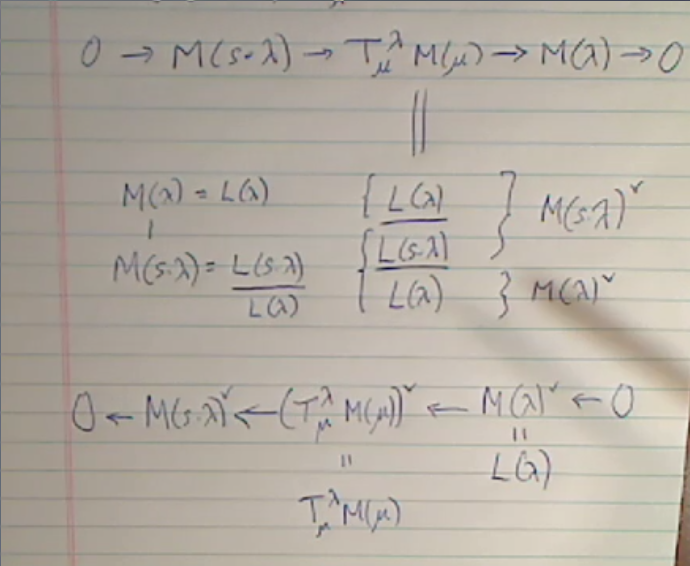
\includegraphics{figures/image_2020-04-24-09-25-20.png}\\

Also recall Proposition 3.7a: If \(M\in \OO\) has a standard filtration
and \(\lambda \in \Pi(M)\) is maximal, then \(M(\lambda) \injects M\)
and \(M/M(\lambda)\) has a standard filtration.

\begin{description}
\item[Theorem (Existence of ``Highest Weight'' Tilting Modules)]
Let \(\lambda \in \Lambda\):

\begin{enumerate}
\def\labelenumi{\alph{enumi}.}
\tightlist
\item
  There exists an indecomposable tilting module
  \(T(\lambda) \in \OO_{\text{int}}\) such that
  \(\dim T(\lambda)_\lambda = 1\) and
  \(\mu \in \Pi(T(\lambda)) \implies \mu \leq \lambda\). In particular,
  \(( T(\lambda): M(\lambda) ) = 1\) and
  \(M(\lambda) \injects T(\lambda)\).
\end{enumerate}

\begin{quote}
Note that this implies that \(T(\lambda)\) must lie in the single block
\(\OO_{\chi_\lambda}\), since it has a Verma \(M(\lambda)\) and is
indecomposable.
\end{quote}

\begin{enumerate}
\def\labelenumi{\alph{enumi}.}
\setcounter{enumi}{1}
\tightlist
\item
  Every indecomposable tilting module in \(\OO_{\text{int}}\) is
  isomorphic to \(T(\lambda)\) for some \(\lambda \in \Lambda\).
\item
  \(T(\lambda)\) is the only tilting module up to isomorphicin
  \(\OO_{\text{int}}\) having the properties in (a).
\item
  \(\theset{[T(\lambda)]}_{\lambda \in \Lambda}\) is a basis for
  \(\mck = K(\OO_{\text{int}})\).
\end{enumerate}
\item[Proof (of (a))]
Existence is by induction on length in \(W\) along with translation to
and from walls. Fix \(\lambda \in \Lambda\) to be \(\rho\dash\)regular
and antidominant. Consider the linked weights \(w\cdot \lambda\) and
their translates to walls. To start, set
\(T(\lambda) \definedas M(\lambda)\) which has the properties in (a).
Likewise for \(\mu \in \bar C\), for \(C\) the antidominant chamber,
\(\mu\) is still antidominant, \(T_\lambda^\mu M(\lambda) = M(\mu)\)
again irreducible and seta \(T(\mu) \definedas M(\mu)\)

For the inductive step, assume \(T(w\cdot \mu)\) has been constructed
for all \(\mu \in \bar{w\cdot C}\) to \(T(w\cdot \lambda)\) is defined.
If \(s\) is a simple reflection with \(ws > w\) choose an antidominant
integral weight \(\mu\) with \(W_{\mu}^0 = \theset{1, s}\) so we have
defined \(T(w\cdot \mu) T(ws \cdot \mu)\). Apply the exact functor
\(T_\mu^\lambda\) and use theorem 7.14: \(T_\mu^\lambda T(w\cdot \mu)\)
has a two-step filtration with sections \begin{align*}
N: {M(w\cdot \lambda) \over M(ws\cdot \lambda)  }
.\end{align*} where the top term is a non-split extension and the bottom
is indecomposable with \(\hd = L(w\cdot \lambda)\).

The other sections \(M(x\cdot \mu)\) of \(T(w\cdot \mu)\) have
\(x\cdot \mu < w\cdot \mu\). Applying \(T_\mu^\lambda\) to these
produces 2-step modules like \(N\) but with highest weights either
\(xs \cdot \lambda < ws\cdot \lambda\), or \(x\cdot \lambda\), whichever
is greater.

\hfill\break

Thus \(ws \cdot \lambda\) is the unique largest weight (occurring with
multiplicity one) in the titling module \(T_\mu^\lambda T(w\cdot \mu)\)
by Prop 11.1e. Set \(T(ws\cdot \lambda)\) to be the indecomposable
summand of this involving the weight \(ws\cdot \lambda\), this has the
required properties in (a).

\hfill\break

We can now translate \(T(ws\cdot \lambda)\) to the walls of
\(\bar{ws\cdot C}\), which were not already walls of \(\bar{w\cdot C}\).
For weights \(\nu\) in such walls, the translated module with have a
1-dim \(\nu\dash\)weight space \(M\) (Theorem 7.6), so we can take the
indecomposable summand containing \(M\) to be \(M(\nu)\), completing the
inductive step.
\item[Proof (of (b))]
Let \(T\) be any indecomposable tilting module having \(\lambda\) as one
of its maximal weights. By the remark concerning Prop 3.7a, there is an
embedding \(M(\lambda) \injects T\) at the bottom of a standard
filtration and \(T/M(\lambda)\) has a standard filtration. Thus
\(\ext^1(T/M(\lambda, T(\lambda))) = 0\), using Prop 11.1f and Exercise
6.12.

Applying \(\hom(\wait, T(\lambda))\) to
\begin{align*}0 \to M(\lambda) \mapsvia{f} T \to T/M(\lambda) \to 0\end{align*}
yields
\begin{align*}\hom(T, T(\lambda)) \mapsvia{f^*} \hom(M(\lambda), T(\lambda)) \to \ext^1(T/M(\lambda), T(\lambda)) = 0 \to \cdots.\end{align*}
Thus \(f_*\) is surjective, and the embedding
\(M(\lambda) \injects T(\lambda)\) lifts to a map
\(\phi: T\to T(\lambda)\):

\begin{center}
\begin{tikzcd}
M(\lambda)
& T \ar[d, dotted, "\phi"]  \\
M(\lambda) \ar[r] 
& T(\lambda) \ar[u, dotted, "\psi"]
\end{tikzcd}
\end{center}

Similarly, reversing \(T, T(\lambda)\) we get the map \(\psi\) with is
the identity on the specified submodules of \(M(\lambda)\) in each. This
we get endomorphisms \(\phi \circ \psi\) of \(T(\lambda)\), which is an
isomorphism on the \(\lambda\dash\)weight space \(T(\lambda)_\lambda\)
and of \(\psi\circ \phi(T)\), which is an isomorphism \emph{at least} on
the \(\CC\dash\) span of \(v_\lambda^+ \in M(\lambda) \subset T\)
(although maybe not on all of \(T_\lambda\) as claim in Humphreys).

By Fitting's lemma (?) an endomorphism of a finite length indecomposable
module is either nilpotent or invertible. But the two compositions can
not be nilpotent since they are isomorphisms on \(\CC v_\lambda^+\)
viewed in \(T(\lambda)\) and in \(T\).
\item[Proof (of (c))]
Take \(T\) to be a tilting module\ldots{}
\end{description}

\hypertarget{monday-april-27th}{%
\section{Monday April 27th}\label{monday-april-27th}}

We get a non-split SES \begin{align*}
0 \to M(xs\cdot \lambda) \to T_\mu^\lambda M(x\cdot \mu) \to M(x\cdot \lambda) \to 0
.\end{align*}

Since \(w\cdot \mu\) is the highest weight of \(T(w\cdot \mu)\) and
occurs with multiplicity one, apply this to all Verma section
\(M(x\cdot \mu)\), including \(x= w\) in a standard filtration of
\(T(w\cdot \mu)\), thus \(T_\mu^\lambda T(w\cdot \mu)\) has highest
weight \(ws\cdot \lambda\) with multiplicity one.

By Prop 11.1e and Theorem 11.2,
\(T_\mu^\lambda T(w\cdot \mu) \cong T(ws \cdot \lambda) \oplus T\) where
\(T\) is a tilting module in \(\OO_{\chi_\lambda}\) having all weights
less than \(ws\cdot \lambda\). It suffices to show \(T=0\), or
equivalently \(T_\lambda^\mu T = 0\).

\begin{description}
\tightlist
\item[Lemma (Translating and Inverting Doubles the Character)]
For \(\lambda, \mu\) as above and any \(M\in \OO_{\chi_\mu}\),
\(\ch T_\lambda^\mu T_\mu^\lambda M = 2 \ch M\).
\end{description}

Proof: By writing \(\ch M\) in a basis of \(M(x\cdot \mu)\) with
\(x\in W\) and \(xs > x\), since \(M(xs \cdot \mu) = M(x \cdot \mu)\),
it suffices to show this for \(M = M(x\cdot \mu)\). But
\(T_\lambda^\mu T_\mu^\lambda M(x\cdot \mu)\) is given by applying
\(T_\lambda^\mu\) to the original SES and we know
\begin{align*}
T_\lambda^\mu M(xs\cdot \lambda) = M(xs \cdot \mu) = M(x\cdot \mu) = T_\lambda^\mu M(x\cdot \lambda)
\end{align*} Thus
\(\ch T_\lambda^\mu T_\mu^\lambda M(x\cdot \mu) = 2\ch M(x\cdot \mu)\).

\(\qed\)

Now by the lemma,
\(T_\lambda^\mu T(ws \cdot \lambda) \oplus T_\lambda^\mu T = T_\lambda^\mu T_\mu^\lambda T(w\cdot \mu)\)
has formal character \(2 \ch T(w\cdot \mu)\). Since it's a tilting
module,we must have
\(T_\lambda^\mu T_\mu^\lambda T(w\cdot \mu) = T(w\cdot \mu) \oplus T(w\cdot \mu)\).
In particular, it has highest weight \(w\cdot \mu\) with multiplicity 2.

If we can show that \(T_\lambda^\mu T(ws\cdot \lambda)\) already has
\(w\cdot \mu\) as a weight with multiplicity 2, it will follow that the
remaining term must be zero as desired.

Start with an embedding
\(\phi: M(ws\cdot \lambda) \injects T(ws\cdot \lambda)\). Using Theorem
6.13c, our \(\ext^1\) vanishes between Vermas and dual Vermas, and so we
have \(\ext^1 (T(ws\cdot \lambda), M(w\cdot\lambda A)\dual) = 0\).

Dualizing, \(\ext^1(M(w\cdot \lambda), T(ws\cdot \lambda)) = 0\) and
this sequence must split. Applying \(\hom(\wait, T(ws\cdot \lambda))\),
we get a LES \begin{align*}
\hom(T_\mu^\lambda M(w\cdot \lambda), T(ws\cdot \lambda)) \to \hom(M(ws\cdot \lambda), T(ws\cdot \lambda)) \to \ext^1(M(w\cdot \lambda), T(ws\cdot\lambda)) \to \cdots
.\end{align*}

Since the last term vanishes, a \(\phi\) in the middle term lifts to the
first term.

\begin{description}
\item[Proposition (Injective Embedding of Vermas into Tilting Modules)]
\((\ker\phi)_{w\cdot \lambda} = 0\).
\item[Proof]
If not, since \(\phi\) restricted to \(M(ws\cdot \lambda)\) is
injective, and using the origin SES we must have a preimage
\(v\in (\ker \phi)_{w\cdot \lambda}\) of the highest weight vector in
\(M(w\cdot \lambda)\).

But every \(z\in T_\mu^\lambda M(w\cdot \mu)\) can be written uniquely
(since the SES splits as vector spaces) as \(z = uv + m\) where
\(u\in U(\lien^-)\) and \(m\in M(ws\cdot \lambda)\). Then
\(\phi(z) = 0 + \phi(m) = m \in M(ws\cdot \lambda) \subset T(ws\cdot\lambda)\),
since \(\phi\) is the identity on this submodule. But then \(\phi\)
provides a splitting of the non-split SES, a contradiction.
\end{description}

Thus \(\phi\) induces a nonzero homomorphism \begin{align*}
\bar \phi : M(w\cdot \lambda) \cong T_\mu^\lambda M(w\cdot \mu) / M(ws\cdot \lambda) \to T(ws\cdot \lambda) / M(ws\cdot \lambda)
.\end{align*}

In particular, \(w\cdot \lambda\) is a weight of the quotient module,
and is a maximal weight -- keeping in mind that \(T(ws\cdot \lambda)\)
has a standard filtration with sections \(M(x\cdot \lambda)\) for
\(x \leq ws\) with \(M(ws\cdot \lambda)\) occurring just once. The
quotient module also has a standard filtration, so \(M(w\cdot \lambda)\)
must occur in the standard filtration of \(T(ws\cdot \lambda)\) along
with \(M(ws\cdot \lambda)\).

Since \(w<ws\), theorem 1.4 provides an injection
\(M(w\cdot \lambda) \injects M(ws\cdot \lambda)\). Applying
\(T_\lambda^\mu\) to these two copies of \(M(w\cdot \lambda)\), we get
\(w\cdot \mu\) a weight with multiplicity at least 2.

\(\qed\)

\begin{description}
\tightlist
\item[Corollary (Standard Multiplicities of Vermas in Tilting Modules)]
Under the hypotheses of the theorem,
\((T(ws\cdot \lambda): M(xs \cdot \lambda)) = (T(ws\cdot \lambda) : M(x\cdot \lambda))\).
\item[Proof]
\(T(ws\cdot \lambda) = T_\mu^\lambda T(w\cdot \mu)\), and wlog
\(x < xs\) since the claimed formula is symmetric in \(x\) and \(xs\)
and \(xs\cdot \mu = x\cdot \mu\). Now tilting modules (and thus their
filtration multiplicities) are determined by their formal characters.
Using 1', we see that each occurrence of \(M(x\cdot \mu)\) as a section
of \(T(w\cdot \mu)\) leads to exactly one occurence of
\(M(xs\cdot \lambda)\) and \(M(x\cdot \lambda)\) in the character of
\(T(ws \cdot \lambda)\).
\end{description}

Remark: Both the theorem and corollary can fail when \(ws<w\).

\newpage

\newpage
\section{Indices}
\listoftodos[List of Todos]

% Hook into amsthm environments to list them.
\renewcommand{\listtheoremname}{Definitions}
\listoftheorems[ignoreall,show={definition}, numwidth=3.5em]

\renewcommand{\listtheoremname}{Theorems}
\listoftheorems[ignoreall,show={theorem,proposition}, numwidth=3.5em]

\renewcommand{\listtheoremname}{Exercises}
\listoftheorems[ignoreall,show={exercise}, numwidth=3.5em]

\listoffigures


\printbibliography[title=Bibliography]


\end{document}
